%%
%DIF LATEXDIFF DIFFERENCE FILE
%DIF DEL orig-flat.tex   Wed Nov 25 18:12:59 2026
%DIF ADD new-flat.tex    Wed Nov 25 18:12:59 2026
%% Mosaic paper repository main file.
%%
% TACO submission version.  ACM journals use the acmsmall trim; `review'
% adds the line numbers reviewers are asked to cite, and `anonymous'
% suppresses author names, affiliations, e-mails, and ORCIDs.
% For the camera-ready version, drop `review,anonymous' and restore the
% author block below.
\documentclass[acmsmall,review,anonymous,screen]{acmart}

\AtBeginDocument{%
  \providecommand\BibTeX{{%
    Bib\TeX}}}

% ACM is fully open access; TACO articles are published under CC-BY.
\setcopyright{cc}
\setcctype{by}
\copyrightyear{2026}
\acmYear{2026}
\acmJournal{TACO}
% Volume/number/article/month and the DOI are assigned by ACM at
% acceptance; they stay as placeholders in the submitted version.
\acmVolume{0}
\acmNumber{0}
\acmArticle{0}
\acmMonth{0}
\acmDOI{10.1145/nnnnnnn.nnnnnnn}
% Paste the submission ID issued by Manuscript Central here; it is then
% printed on every page under the `review' option.
\acmSubmissionID{}

% User-defined packages.
\usepackage{xspace}
\usepackage{graphicx}
\usepackage{pgfplots}
\pgfplotsset{compat=1.17}
\usepackage{booktabs}
\usepackage{siunitx}
\usepackage{multirow}
\usepackage{makecell}
\usepackage{adjustbox}
\usepackage{array}
\usepackage{tabularx}
\usepackage{placeins}
\usepackage{enumitem}
\usepgfplotslibrary{statistics, groupplots}
\usetikzlibrary{shapes.geometric, arrows.meta, positioning, fit, backgrounds, positioning, calc, matrix, backgrounds}
\definecolor{primaryblue}{RGB}{70,130,180}
\definecolor{accentorange}{RGB}{255,140,0}
\definecolor{deepgreen}{RGB}{34,139,34}
\definecolor{deepskyblue}{RGB}{46,84,161}
\definecolor{mypurple}{RGB}{112, 48, 160}
\definecolor{lightblue}{RGB}{173, 216, 230}
\definecolor{lightpurple}{RGB}{221, 160, 221}
\definecolor{lightpink}{RGB}{255, 182, 193}
\definecolor{color1}{RGB}{199,56,73}
\definecolor{color2}{RGB}{248,189,211}
\definecolor{color3}{RGB}{191,170,210}
\definecolor{color4}{RGB}{147,197,235}
\definecolor{color5}{RGB}{157,159,163}
%DIF 61a61-91
\newif\ifrevmarkup %DIF >
\revmarkuptrue %DIF >
\ifdefined\revclean\revmarkupfalse\fi %DIF >
\definecolor{revO}{HTML}{7030A0} %DIF >
\DeclareRobustCommand{\revO}[1]{\ifrevmarkup{\color{revO}\hypersetup{allcolors=revO}#1}\else#1\fi} %DIF >
\newenvironment{revOblock}{\ifrevmarkup\color{revO}\hypersetup{allcolors=revO}\fi}{} %DIF >
\definecolor{revRone}{HTML}{0070C0} %DIF >
\DeclareRobustCommand{\revRone}[1]{\ifrevmarkup{\color{revRone}\hypersetup{allcolors=revRone}#1}\else#1\fi} %DIF >
\newenvironment{revRoneblock}{\ifrevmarkup\color{revRone}\hypersetup{allcolors=revRone}\fi}{} %DIF >
\definecolor{revRtwo}{HTML}{C00000} %DIF >
\DeclareRobustCommand{\revRtwo}[1]{\ifrevmarkup{\color{revRtwo}\hypersetup{allcolors=revRtwo}#1}\else#1\fi} %DIF >
\newenvironment{revRtwoblock}{\ifrevmarkup\color{revRtwo}\hypersetup{allcolors=revRtwo}\fi}{} %DIF >
\definecolor{revRthree}{HTML}{00B050} %DIF >
\DeclareRobustCommand{\revRthree}[1]{\ifrevmarkup{\color{revRthree}\hypersetup{allcolors=revRthree}#1}\else#1\fi} %DIF >
\newenvironment{revRthreeblock}{\ifrevmarkup\color{revRthree}\hypersetup{allcolors=revRthree}\fi}{} %DIF >
\ifrevmarkup\else %DIF >
  \AtBeginDocument{% %DIF >
    \hypersetup{hidelinks}% %DIF >
    \tikzset{every text node part/.append style={text=black}}} %DIF >
  \makeatletter %DIF >
  \patchcmd{\ACM@mk@linecount}{\color{red}}{\color{black}}{}{} %DIF >
  \patchcmd{\ACM@mk@linecount}{\color{red}}{\color{black}}{}{} %DIF >
  \makeatother %DIF >
\fi %DIF >
\makeatletter %DIF >
\pdfstringdefDisableCommands{% %DIF >
  \let\revO\@firstofone\let\revRone\@firstofone %DIF >
  \let\revRtwo\@firstofone\let\revRthree\@firstofone} %DIF >
\makeatother %DIF >
 %DIF >
 %DIF >
%DIF -------
\usepackage[utf8]{inputenc}
\usepackage{algorithm}
%DIF 63c94
%DIF < \usepackage[noend]{algpseudocode}
%DIF -------
\usepackage{algpseudocode} %DIF >
%DIF -------
\usepackage{wrapfig}
% Apply the layout rhythm after acmart installs its document-level defaults.
\AtBeginDocument{%
  \setlength{\intextsep}{8pt plus 2pt minus 2pt}%
  \setlength{\textfloatsep}{4pt plus 1pt minus 1pt}%
  \setlength{\floatsep}{8pt plus 2pt minus 2pt}%
  \setlength{\dbltextfloatsep}{8pt plus 2pt minus 2pt}%
  \setlength{\dblfloatsep}{8pt plus 2pt minus 2pt}%
  \setlength{\abovedisplayskip}{4.2pt plus 1pt}%
  \setlength{\belowdisplayskip}{4.2pt plus 1pt}%
  \setlength{\abovedisplayshortskip}{0pt plus 1pt}%
  \setlength{\belowdisplayshortskip}{2.1pt plus 1pt}%
  \setlength{\jot}{4pt}%
}
\usepackage{listings}
\definecolor{darkgray}{rgb}{.3,.3,.3}
\definecolor{darkred}{rgb}{.6,0,0}
\definecolor{darkgreen}{rgb}{0,.6,0}
\definecolor{darkblue}{rgb}{0,0,.6}
\definecolor{codegreen}{rgb}{0,0.6,0}
\definecolor{codegray}{rgb}{0.5,0.5,0.5}
\definecolor{codepurple}{rgb}{0.58,0,0.82}
\definecolor{backcolour}{rgb}{0.95,0.95,0.92}
\lstdefinestyle{patterncode}{
  language=Python,
  basicstyle=\ttfamily\scriptsize,
  keywordstyle=\bfseries\color{black},
  commentstyle=\itshape\color{gray!65},
  stringstyle=\color{black},
  showstringspaces=false,
  breaklines=false,
  frame=single,
  framerule=0.4pt,
  xleftmargin=6pt,
  xrightmargin=6pt,
  aboveskip=2pt,
  belowskip=0pt,
  escapeinside={(*@}{@*)},
  morekeywords={zeros,conv,split,cat,sigmoid,tanh},
}

\newtheorem{definition}{Definition}
\newtheorem{theorem}{Theorem}

\def\sectionautorefname{\S}
\def\subsectionautorefname{\S}
\def\subsubsectionautorefname{\S}
\def\equationautorefname{Eq.}
\def\figureautorefname{Fig.}
\def\tableautorefname{Tab.}
\def\algorithmautorefname{Alg.}
\newcommand{\definitionautorefname}{Def.}
\newcommand{\name}{{Mosaic}\xspace}
\newcommand{\gpu}{GPU\xspace}
\newcommand{\gpus}{GPUs\xspace}
\newcommand{\sm}{SM\xspace}
\newcommand{\sms}{SMs\xspace}
\newcommand{\circled}[1]{\textup{\scriptsize(#1)}}
\newcommand{\tile}{t}
\newcommand{\tvec}{\mathbf{t}}
\newcommand{\rblk}{r}
\newcommand{\rvec}{\mathbf{r}}
\newcommand{\work}{w}
\newcommand{\placement}{\textsc{Placement}\xspace}
\newcommand{\Solve}{\textsc{Solve}}
\newcommand{\Rsm}{R_{\mathrm{SM}}}
\newcommand{\Ssm}{S_{\mathrm{SM}}}
\newcommand{\Sblock}{S_{\mathrm{block}}}
\newcommand{\Bsm}{B_{\mathrm{SM}}}
\newcommand{\Tsm}{T_{\mathrm{SM}}}
\newcommand{\Nsm}{N_{\mathrm{SM}}}
\newcommand{\Tmax}{T_{\max}}
\newcommand{\Wwarp}{w_{\mathrm{warp}}}
\newcommand{\gcoal}{g_{\mathrm{coal}}}
\newcommand{\Lg}{\Lambda_{\mathrm g}}
\newcommand{\Ls}{\Lambda_{\mathrm s}}
\newcommand{\Lr}{\Lambda_{\mathrm r}}
\newcommand{\Lf}{\Lambda_{\mathrm f}}
\newcommand{\Ly}{\Lambda_{\mathrm y}}
\newcommand{\Lglobal}{\Lg}
\newcommand{\Lsmem}{\Ls}
\newcommand{\Lreg}{\Lr}
\newcommand{\Lfma}{\Lf}
\newcommand{\Lsync}{\Ly}
\newcommand{\Czero}{C_0}
\newcommand{\Cinit}{C_{\mathrm{init}}}
\newcommand{\cfma}{c_{\mathrm{fma}}}
\newcommand{\creg}{c_{\mathrm{reg}}}
\newcommand{\Sigmacand}{\Sigma_{\mathrm{cand}}}

% TACO requires an unnumbered footnote on the first page stating the
% relationship of the submission to any prior conference paper.  acmart's
% \titlenote and \thanks both replace their argument with a placeholder under
% the `anonymous' option, so the note is emitted directly instead; it carries
% no author-identifying information and is therefore safe to keep anonymous.
\makeatletter
\newcommand{\firstpagefootnote}[1]{%
  \begingroup
  \renewcommand\thefootnote{}%
  \renewcommand\@makefnmark{}%
  \footnotetext{#1}%
  \addtocounter{footnote}{-1}%
  \endgroup}
\makeatother

% Suppress the page-1 copyright/permission footnote block for this
% submission-stage draft: none of the CC-BY icon+license text, the copyright
% line, the DOI, or the ACM permission-code/article line it prints are
% assigned until acceptance, so showing them here would only display
% placeholders. \setcopyright{cc}/\setcctype{by}/\acmDOI above still record
% the intended camera-ready values; delete this redefinition (restoring
% acmart's default \footnotetextcopyrightpermission) once ACM assigns them.
\makeatletter
\renewcommand\footnotetextcopyrightpermission[1]{}
\makeatother
%DIF PREAMBLE EXTENSION ADDED BY LATEXDIFF
%DIF UNDERLINE PREAMBLE %DIF PREAMBLE
\RequirePackage[normalem]{ulem} %DIF PREAMBLE
\RequirePackage{color}\definecolor{RED}{rgb}{1,0,0}\definecolor{BLUE}{rgb}{0,0,1} %DIF PREAMBLE
\providecommand{\DIFadd}[1]{{\protect\color{blue}\uwave{#1}}} %DIF PREAMBLE
\providecommand{\DIFdel}[1]{{\protect\color{red}\sout{#1}}}                      %DIF PREAMBLE
%DIF SAFE PREAMBLE %DIF PREAMBLE
\providecommand{\DIFaddbegin}{} %DIF PREAMBLE
\providecommand{\DIFaddend}{} %DIF PREAMBLE
\providecommand{\DIFdelbegin}{} %DIF PREAMBLE
\providecommand{\DIFdelend}{} %DIF PREAMBLE
\providecommand{\DIFmodbegin}{} %DIF PREAMBLE
\providecommand{\DIFmodend}{} %DIF PREAMBLE
%DIF FLOATSAFE PREAMBLE %DIF PREAMBLE
\providecommand{\DIFaddFL}[1]{\DIFadd{#1}} %DIF PREAMBLE
\providecommand{\DIFdelFL}[1]{\DIFdel{#1}} %DIF PREAMBLE
\providecommand{\DIFaddbeginFL}{} %DIF PREAMBLE
\providecommand{\DIFaddendFL}{} %DIF PREAMBLE
\providecommand{\DIFdelbeginFL}{} %DIF PREAMBLE
\providecommand{\DIFdelendFL}{} %DIF PREAMBLE
\newcommand{\DIFscaledelfig}{0.5}
%DIF HIGHLIGHTGRAPHICS PREAMBLE %DIF PREAMBLE
\RequirePackage{settobox} %DIF PREAMBLE
\RequirePackage{letltxmacro} %DIF PREAMBLE
\newsavebox{\DIFdelgraphicsbox} %DIF PREAMBLE
\newlength{\DIFdelgraphicswidth} %DIF PREAMBLE
\newlength{\DIFdelgraphicsheight} %DIF PREAMBLE
% store original definition of \includegraphics %DIF PREAMBLE
\LetLtxMacro{\DIFOincludegraphics}{\includegraphics} %DIF PREAMBLE
\newcommand{\DIFaddincludegraphics}[2][]{{\color{blue}\fbox{\DIFOincludegraphics[#1]{#2}}}} %DIF PREAMBLE
\newcommand{\DIFdelincludegraphics}[2][]{% %DIF PREAMBLE
\sbox{\DIFdelgraphicsbox}{\DIFOincludegraphics[#1]{#2}}% %DIF PREAMBLE
\settoboxwidth{\DIFdelgraphicswidth}{\DIFdelgraphicsbox} %DIF PREAMBLE
\settoboxtotalheight{\DIFdelgraphicsheight}{\DIFdelgraphicsbox} %DIF PREAMBLE
\scalebox{\DIFscaledelfig}{% %DIF PREAMBLE
\parbox[b]{\DIFdelgraphicswidth}{\usebox{\DIFdelgraphicsbox}\\[-\baselineskip] \rule{\DIFdelgraphicswidth}{0em}}\llap{\resizebox{\DIFdelgraphicswidth}{\DIFdelgraphicsheight}{% %DIF PREAMBLE
\setlength{\unitlength}{\DIFdelgraphicswidth}% %DIF PREAMBLE
\begin{picture}(1,1)% %DIF PREAMBLE
\thicklines\linethickness{2pt} %DIF PREAMBLE
{\color[rgb]{1,0,0}\put(0,0){\framebox(1,1){}}}% %DIF PREAMBLE
{\color[rgb]{1,0,0}\put(0,0){\line( 1,1){1}}}% %DIF PREAMBLE
{\color[rgb]{1,0,0}\put(0,1){\line(1,-1){1}}}% %DIF PREAMBLE
\end{picture}% %DIF PREAMBLE
}\hspace*{3pt}}} %DIF PREAMBLE
} %DIF PREAMBLE
\LetLtxMacro{\DIFOaddbegin}{\DIFaddbegin} %DIF PREAMBLE
\LetLtxMacro{\DIFOaddend}{\DIFaddend} %DIF PREAMBLE
\LetLtxMacro{\DIFOdelbegin}{\DIFdelbegin} %DIF PREAMBLE
\LetLtxMacro{\DIFOdelend}{\DIFdelend} %DIF PREAMBLE
\DeclareRobustCommand{\DIFaddbegin}{\DIFOaddbegin \let\includegraphics\DIFaddincludegraphics} %DIF PREAMBLE
\DeclareRobustCommand{\DIFaddend}{\DIFOaddend \let\includegraphics\DIFOincludegraphics} %DIF PREAMBLE
\DeclareRobustCommand{\DIFdelbegin}{\DIFOdelbegin \let\includegraphics\DIFdelincludegraphics} %DIF PREAMBLE
\DeclareRobustCommand{\DIFdelend}{\DIFOaddend \let\includegraphics\DIFOincludegraphics} %DIF PREAMBLE
\LetLtxMacro{\DIFOaddbeginFL}{\DIFaddbeginFL} %DIF PREAMBLE
\LetLtxMacro{\DIFOaddendFL}{\DIFaddendFL} %DIF PREAMBLE
\LetLtxMacro{\DIFOdelbeginFL}{\DIFdelbeginFL} %DIF PREAMBLE
\LetLtxMacro{\DIFOdelendFL}{\DIFdelendFL} %DIF PREAMBLE
\DeclareRobustCommand{\DIFaddbeginFL}{\DIFOaddbeginFL \let\includegraphics\DIFaddincludegraphics} %DIF PREAMBLE
\DeclareRobustCommand{\DIFaddendFL}{\DIFOaddendFL \let\includegraphics\DIFOincludegraphics} %DIF PREAMBLE
\DeclareRobustCommand{\DIFdelbeginFL}{\DIFOdelbeginFL \let\includegraphics\DIFdelincludegraphics} %DIF PREAMBLE
\DeclareRobustCommand{\DIFdelendFL}{\DIFOaddendFL \let\includegraphics\DIFOincludegraphics} %DIF PREAMBLE
%DIF LISTINGS PREAMBLE %DIF PREAMBLE
\RequirePackage{listings} %DIF PREAMBLE
\RequirePackage{color} %DIF PREAMBLE
\lstdefinelanguage{DIFcode}{ %DIF PREAMBLE
%DIF DIFCODE_UNDERLINE %DIF PREAMBLE
  moredelim=[il][\color{red}\sout]{\%DIF\ <\ }, %DIF PREAMBLE
  moredelim=[il][\color{blue}\uwave]{\%DIF\ >\ } %DIF PREAMBLE
} %DIF PREAMBLE
\lstdefinestyle{DIFverbatimstyle}{ %DIF PREAMBLE
	language=DIFcode, %DIF PREAMBLE
	basicstyle=\ttfamily, %DIF PREAMBLE
	columns=fullflexible, %DIF PREAMBLE
	keepspaces=true %DIF PREAMBLE
} %DIF PREAMBLE
\lstnewenvironment{DIFverbatim}{\lstset{style=DIFverbatimstyle}}{} %DIF PREAMBLE
\lstnewenvironment{DIFverbatim*}{\lstset{style=DIFverbatimstyle,showspaces=true}}{} %DIF PREAMBLE
%DIF END PREAMBLE EXTENSION ADDED BY LATEXDIFF

\begin{document}

% Previous title read as a comparative claim against transformation scheduling
% ("Beyond Schedule Search"), which contradicts the scope statement in
% sec.intro.tex/sec.conclusion.tex: \name operates strictly after scheduling and
% neither searches nor modifies it. Retitled to name the paper's own subject,
% GPU execution space optimization, instead.
% \title{\name: Unified Analytical Optimization of Architecture-Aware GPU Code Generation Beyond Schedule Search}
\title[Analytical Optimization of Architecture-Aware GPU Code Generation]
{Unified Analytical Optimization of Architecture-Aware GPU Execution Space}

\author{Shihan Yuan}
\email{yuanshihan516@hnu.edu.cn}
\orcid{0009-0005-9508-1660}
\author{Junhui Peng}
\email{pengjh0111@hnu.edu.cn}
\orcid{0009-0006-7218-1930}
\author{Guanghui Song}
\email{sheensong@hnu.edu.cn}
\orcid{0009-0001-8089-1151}
\author{Feng Wang}
\email{wangfeng@hnu.edu.cn}
\orcid{0009-0002-4009-6783}
\author{Kenli Li}
\email{lkl@hnu.edu.cn}
\orcid{0000-0002-2635-7716}
\author{Jie Zhao}
\email{jiezhao@hnu.edu.cn}
\orcid{0000-0003-2303-9736}
\affiliation{%
  \institution{Hunan University}
  \city{Changsha}
  \country{China}
}


\begin{abstract}
Selecting tile sizes and thread-block dimensions is critical to the performance of compiler-generated GPU code, yet these choices interact with shared-memory use, register pressure, occupancy, and memory locality. Existing analytical selectors address narrower subsets of this execution space, while empirical methods incur repeated search costs.

This paper presents \name, a unified analytical framework for GPU execution-space optimization on transformed programs whose schedule and mapping structure have been fixed upstream. \name selects tile and thread-block parameters while reasoning over abstract shared-memory placement scenarios using compiler-provided metadata and a once-per-architecture target profile. Its model combines a quantized wave objective, a shared-read-per-FMA ratio, and a conservative register-working-set filter, followed by a relaxed-cost tie-break among configurations tied at the primary optimum. The formulation also yields a closed-form balanced register-blocking condition for outer-product contractions.

Across 25 PolyBench kernels on three NVIDIA GPUs, \name achieves geometric-mean speedups of $1.21$--$1.49\times$ over PPCG and measured latency ratios of $1.37$--$1.89\times$ relative to \DIFaddbegin \revO{the energy-aware }\DIFaddend EATSS. On the RTX 4090, \name achieves $1.88\times$ over PPCG on deep learning operators and $4.22\times$ over PPCG on end-to-end workloads; on the evaluated end-to-end workloads, it achieves a $1.11\times$ geometric-mean speedup over \DIFaddbegin \revRthree{the parameters tuned by }\DIFaddend TVM MetaSchedule. \name further reduces selection overhead by $12$--$14\times$ relative to EATSS and by $2$--$4$ orders of magnitude relative to measurement-driven autotuning.
\end{abstract}

\begin{CCSXML}
<ccs2012>
   <concept>
       <concept_id>10010520.10010521.10010528</concept_id>
       <concept_desc>Computer systems organization~Parallel architectures</concept_desc>
       <concept_significance>500</concept_significance>
       </concept>
   <concept>
       <concept_id>10011007.10011006.10011008</concept_id>
       <concept_desc>Software and its engineering~General programming languages</concept_desc>
       <concept_significance>300</concept_significance>
       </concept>
   <concept>
       <concept_id>10002950.10003624.10003625.10003630</concept_id>
       <concept_desc>Mathematics of computing~Combinatorial optimization</concept_desc>
       <concept_significance>300</concept_significance>
       </concept>
 </ccs2012>
\end{CCSXML}

\ccsdesc[500]{Computer systems organization~Parallel architectures}
\ccsdesc[300]{Software and its engineering~General programming languages}
\ccsdesc[300]{Mathematics of computing~Combinatorial optimization}

\keywords{GPU Code Generation, Execution Space Optimization, Analytical Model, Polyhedral Compilation}

\maketitle

% Mandatory TACO first-page footnote.  Replace with a citation of the prior
% conference paper plus a statement of the >=30% new material if this ever
% becomes an extension rather than a new paper.
\firstpagefootnote{New Paper, Not an Extension of a Conference Paper.}

% !TEX root =  mosaic.tex
\section{Introduction}
\label{sec:intro}

\gpus are the dominant execution platform for scientific computing, machine learning, and data analytics. To target them, modern compilers automatically apply loop transformations such as fusion, distribution, interchange, skewing, and tiling: polyhedral frameworks~\DIFdelbegin \DIFdel{\mbox{%DIFAUXCMD
\cite{ppcg,pluto,polly,tc,akg} }\hspace{0pt}%DIFAUXCMD
}\DIFdelend \DIFaddbegin {\hypersetup{citecolor=black}[\citenum{pluto}, \citenum{polly}, \citenum{tc}, \citenum{ppcg}, \revO{\citenum{zhao2020micro}}, \citenum{akg}, \revO{\citenum{zhao2024tocs}}]} \DIFaddend derive these transformations through dependence analysis, while deep learning compilers like Halide~\cite{halide} and TVM~\cite{tvm} expose scheduling primitives that can be explored or tuned.

Transformation scheduling has been extensively explored in these systems, but efficient \gpu code generation also depends on architecture-specific execution parameters that remain after, or are chosen alongside, scheduling. Once a schedule and its mapping structure are fixed, the compiler must still choose tile sizes and thread-block dimensions that govern how the transformed computation consumes shared memory, registers, caches, and streaming multiprocessors (SMs). Unlike loop transformations, which reshape the iteration space and computation order, execution-space optimization leaves them intact and selects resource parameters exposed by the resulting schedule. These decisions therefore complement transformation scheduling rather than replace it.

Prior work on these execution parameters follows two broad lines: analytical selection and empirical search. Analytical tile size selection originated on CPUs, choosing tiles so a footprint stays resident in cache~\cite{mckinley-tss,lam-tss} and later embedding this reasoning in polyhedral~\cite{pluto-tss}, geometric programming~\cite{rajopadhye-gp,rajopadhye-igp}, and decoupled~\cite{tilemind} formulations. \gpu-specific analytical approaches include models derived for individual kernel classes such as matrix multiplication, convolution, or BLAS~\cite{li-gemm,saday-conv,blis}, compiler-integrated tile selection~\cite{ppcg-tss}, and EATSS~\cite{eatss}, which analytically selects \gpu tile sizes under a joint latency--energy objective. Empirical approaches, including autotuners~\cite{metaschedule,ansor,automatichalide} and learning-based pruning~\cite{hctuner,shirako-tss,yuki-tss}, instead explore candidate configurations through measurement or prediction and incur repeated tuning costs for new targets or shapes.

We formulate execution-space selection on a fixed transformed schedule: choosing tile sizes and thread-block dimensions while reasoning over abstract shared-memory placement scenarios and coupled \gpu resource effects. \name uses a compiler-agnostic metadata interface populated by compiler-specific adapters. The execution-space unknowns are coupled: the per-thread register budget depends on the resident-block count, which itself depends on register usage; staging an operand in shared memory cuts global traffic but consumes capacity and can lower the resident-block count; an SM hosts an integer number of blocks, so the grid runs in a discrete number of waves whose boundaries move with tile and placement choices; and the exact register count is fixed by the backend allocator only after code generation.

Our key insight is that these interactions can be captured by two compact quantities whose interaction is what makes the landscape irregular: a \emph{quantized wave cost}, a per-block cost multiplied by an integer wave count, which reproduces the step-function discontinuities that smooth objectives miss, and a \emph{shared-read-per-FMA ratio}, which normalizes operand reads by the arithmetic they serve and exposes register blocking as the lever trading locality against register pressure. Around these, a conservative register-working-set filter rejects only configurations whose register lower bound already exceeds the budget, breaking the occupancy--register cycle by reasoning rather than measurement.

We realize this insight in \name, which operates on the transformed programs emitted by existing schedulers~\cite{ppcg,tvm}. \name selects tile sizes and thread-block dimensions while reasoning over abstract shared-memory placement scenarios and accounting for occupancy and register pressure. It enumerates these scenarios around a two-stage analytical selection with a quantized primary objective and a relaxed-cost tie-break over the Stage-1 optimal discrete configurations, recovering balanced register blocking for outer-product contractions as an analytical outcome rather than an imposed rule. \name sits strictly between transformation scheduling and backend code generation: an upstream compiler first fixes a legal transformation schedule and mapping structure---i.e., which dimensions are assigned to block and thread axes---while \name selects the tile sizes and thread-block dimensions that this structure leaves open. It neither searches nor modifies the schedule or mapping structure. Our current cost model targets conventional CUDA-core SIMT execution, as exercised by the PPCG and non-tensorized TVM paths evaluated in this work; we return to this scope boundary in \autoref{sec:conclusion}.

This distinguishes \name from the prior approaches above: unlike heuristic polyhedral code generation~\cite{ppcg}, it selects execution parameters through an architecture-aware analytical model; unlike kernel-specific \gpu models~\cite{li-gemm,saday-conv,blis}, it spans reductions, contractions, and stencils; unlike prior analytical tile-size selection approaches~\cite{ppcg-tss,eatss,pluto-tss}, it combines placement-aware analytical reasoning with register feasibility and wave quantization; and unlike autotuners~\cite{ansor,metaschedule}, it derives interpretable configurations once, with no per-shape or per-target tuning loop. The evaluation in \autoref{sec:eval} confirms that this analytical reasoning replaces a substantial portion of \gpu execution-space autotuning.

In summary, this work makes the following contributions:
\begin{itemize}
  \item We formulate \gpu execution-space selection as a distinct post-scheduling optimization problem in GPU code generation, complementary to transformation scheduling.
  \item We propose \name, a unified analytical model that selects tile sizes and thread-block dimensions while reasoning over abstract shared-memory placement scenarios and accounting for occupancy and register pressure, closing the coupled feedback loop in one solvable formulation and yielding balanced register blocking as a closed-form optimum for outer-product contractions.
  \item We design a compiler-agnostic analytical core with compiler-specific metadata adapters that operates on transformed programs and integrates with polyhedral schedulers, template-based code generators, and autotuning systems.
  \item We evaluate \name with a cross-generation PolyBench/C~\cite{polybench} study on three NVIDIA \gpus, together with deep learning operators and end-to-end workloads on the RTX 4090, showing aggregate gains over heuristics and analytical selectors and competitive performance with a state-of-the-art autotuner without measurement-driven execution-space search.
\end{itemize}

% !TEX root =  mosaic.tex
\section{Background and Motivation}
\label{sec:background}

\subsection{GPU Execution Space Decisions}
\label{sec:bg-decisions}
\label{sec:gpu-execution-model}

A GPU kernel launches a grid of thread blocks; each block runs on an SM whose resident-block count is limited by block/thread limits, per-block shared memory, and per-thread registers. Under the compiler-provided mapping, \name selects tile sizes and thread-block dimensions while reasoning over abstract shared-memory placement scenarios and accounting for occupancy and register pressure (\autoref{sec:intro}). Larger tiles improve reuse but grow footprint and live state, while smaller tiles raise occupancy but expose less locality. As each tile or modeled placement scenario moves several of these limits at once, they cannot be treated as independent dials.

\name does not perform transformation scheduling. It starts from a transformed program whose legal order is fixed by an existing scheduler: schedule trees and affine accesses for polyhedral compilers~\cite{ppcg,tc}, or schedule traces and tensor metadata for template compilers~\cite{halide,tvm}. From this representation, \name extracts loop extents, schedule annotations, access footprints, read/write polarity, operation counts, and coalescing layout, enough to classify dimensions and array roles without depending on compiler internals.


%\subsection{Why Execution Space Parameters Matter}
%\label{sec:bg-why}
%\label{sec:execution space-motivation}

% Reserve enough wrapped lines for the full caption plus the same clear
% post-float separation used after Fig. 2; the shorter reservation allowed the
% following full-width line to intrude into the last caption line.
\begin{wrapfigure}[26]{R}{0.49\textwidth}
  \centering
  \includegraphics[width=\linewidth]{figure1_main.pdf}
  \caption{GEMM execution space landscape on RTX 4090 under a fixed schedule. (a) Log-ratio runtime for configurations that successfully launch, with measured and predicted optima marked. (b) One-dimensional slice at \name's selected block-thread count, showing measured runtime as a function of the per-thread workload.}
  \Description{Measured performance landscape for GPU GEMM execution space configurations.}
  \label{fig:motivation-landscape}
  \par\addvspace{\medskipamount}
\end{wrapfigure}

To make the case concrete, we hold one GEMM (general matrix multiplication) schedule fixed, the running example detailed in \autoref{fig:gemm-schedule-metadata}, and sweep only tile sizes along the output dimensions and thread-block dimensions. These changes can induce different concrete shared-memory staging choices through PPCG's backend lowering. Of 5,000 candidate configurations, 2,232 launch successfully; PPCG~\cite{ppcg} emits each kernel and we measure its time on an RTX 4090, with \autoref{fig:motivation-landscape} plotting the result.

\subsection{Motivating Observation}
\label{sec:bg-repr}
\label{sec:program-representation}

Under this fixed schedule, execution space selection alone moves runtime by over an order of magnitude, and only 28 of the launched configurations (1.25\%) fall within 10\% of the best. Tile size, block shape, and the backend staging they induce therefore remain consequential even once the schedule is fixed, rather than a residual choice left to a simple heuristic. \autoref{fig:motivation-landscape}(a) shows an irregular, non-convex surface on which \name's analytical selection still lands within 10\% of the measured optimum. \autoref{fig:motivation-landscape}(b) fixes the per-block thread count to \name's choice and isolates the per-thread workload, the number of output elements each thread computes, set by the register-blocking factor (\autoref{sec:abstraction}). With the thread count fixed, a tile still splits across threads in several ways, so this workload stays a free variable; the slice shows it alone moves runtime substantially, making register blocking a first-order decision rather than a residual tie break.

\subsection{GPU-Specific Modeling Challenges}
\label{sec:bg-challenges}
\label{sec:gpu-modeling-challenges}

\label{sec:challenge-register-cycle}
\label{sec:challenge-placement}
\label{sec:challenge-discrete-objective}
\label{sec:challenge-register-pressure}

Analytical execution-space optimization must address four GPU-specific challenges. First, occupancy and register budget form a circular dependence: the per-thread register budget depends on the resident-block count, which itself depends in part on register usage, and an analytical model cannot compile each candidate to read back achieved occupancy. Second, abstract shared-memory placement-scenario reasoning is coupled with tile selection: staging a read-only operand cuts predicted global traffic but consumes capacity and may lower the resident-block count, so modeled scenarios must be evaluated alongside tile size, block shape, and reuse pattern. Third, wave counts are discretely quantized: an SM hosts an integer number of blocks, so a grid executes in a discrete number of waves whose ceiling shifts with tile and scenario choices, producing step boundaries no smooth objective captures. Finally, register pressure is unknown before code generation, since the exact count is set by the backend allocator afterward, so a sound model needs a conservative compile-time feasibility filter.

These four effects are therefore not independent knobs but one coupled feedback loop: footprint, resident blocks, register budget, and wave count move together, so they must be resolved jointly in a single formulation rather than by a sequence of independent heuristics.

% !TEX root =  mosaic.tex
\section{Overview of \name}
\label{sec:overview}

\name treats the transformed program as the boundary between transformation scheduling and execution-space optimization: existing schedulers fix the legal computation order and mapping structure, and \name selects only the tile sizes \(\tvec\) and thread-block dimensions \(\mathbf{b}\) that this structure leaves open while reasoning over abstract shared-memory placement scenarios \(S\) and accounting for occupancy and register pressure. Throughout, \name operates outside the compiler; the backend is driven as a black box and all resource reasoning happens in \name. As summarized in \autoref{fig:mosaic-pipeline}, the workflow comprises four components:

% Required in the preamble:
% \usepackage{tikz}
% \usetikzlibrary{arrows.meta,fit,positioning,calc,backgrounds,matrix}
%
% Palette used by this figure:
\definecolor{color1}{RGB}{199,56,73}
\definecolor{color2}{RGB}{248,189,211}
\definecolor{color3}{RGB}{191,170,210}
\definecolor{color4}{RGB}{147,197,235}
\definecolor{color5}{RGB}{157,159,163}

\begin{figure*}[!tbp]
\centering
\begin{adjustbox}{max width=\textwidth}
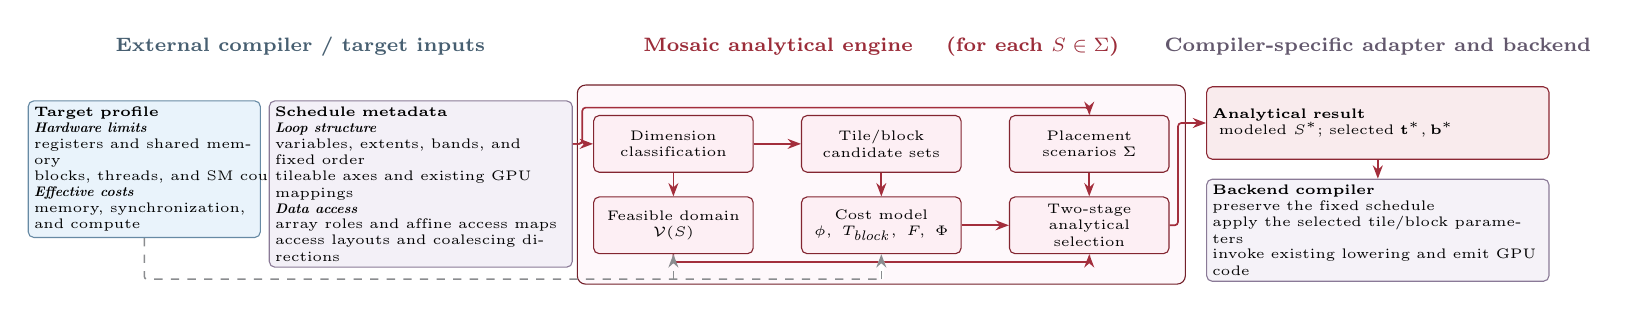
\begin{tikzpicture}[
  font=\tiny,
  >={Stealth[length=1.7mm]},
  box/.style={
    rectangle,
    rounded corners=2pt,
    draw=color5!82!black,
    align=left,
    inner sep=2.1pt,
    minimum height=11mm
  },
  input/.style={
    box,
    fill=color3!18,
    draw=color3!72!black,
    text width=37mm
  },
  target/.style={
    box,
    fill=color4!20,
    draw=color4!70!black,
    text width=28mm
  },
  stage/.style={
    box,
    fill=color2!24,
    draw=color1!66!black,
    align=center,
    text width=16mm,
    minimum height=7.2mm,
    inner sep=1.8pt
  },
  selected/.style={
    box,
    fill=color1!10,
    draw=color1!70!black,
    text width=42mm,
    minimum height=9.2mm
  },
  backend/.style={
    box,
    fill=color3!15,
    draw=color3!72!black,
    text width=42mm,
    minimum height=9.2mm
  },
  title/.style={
    font=\scriptsize\bfseries,
    align=center
  },
  arr/.style={
    ->,
    line width=0.6pt,
    draw=color1!82!black
  },
  darr/.style={
    ->,
    line width=0.55pt,
    dashed,
    draw=color5!88!black
  },
  dline/.style={
    line width=0.55pt,
    dashed,
    draw=color5!88!black
  },
]

% ------------------------------------------------------------------
% External compiler / target inputs
% ------------------------------------------------------------------
\matrix (inputboxes) [
  matrix of nodes,
  nodes in empty cells,
  column sep=1mm,
  inner sep=0pt,
  anchor=west
] {
  \node[target] (prof) {%
    \textbf{Target profile}\\[-0.2pt]
    \textbf{\textit{Hardware limits}}\\[-0.3pt]
    registers and shared memory\\[-0.3pt]
    \mbox{blocks, threads, and SM count}\\[-0.2pt]
    \textbf{\textit{Effective costs}}\\[-0.3pt]
    memory, synchronization, and compute};
  &
  \node[input] (sched) {%
    \textbf{Schedule metadata}\\[-0.2pt]
    \textbf{\textit{Loop structure}}\\[-0.3pt]
    variables, extents, bands, and fixed order\\[-0.3pt]
    tileable axes and existing GPU mappings\\[-0.2pt]
    \textbf{\textit{Data access}}\\[-0.3pt]
    array roles and affine access maps\\[-0.3pt]
    access layouts and coalescing directions};
  \\
};

\begin{scope}[on background layer]
  \node[
    fit=(prof)(sched),
    inner sep=0pt
  ] (inputgroup) {};
\end{scope}

% ------------------------------------------------------------------
% \name analytical engine
% ------------------------------------------------------------------
\node[stage, text width=19mm, anchor=west]
  (cls)
  at ([xshift=2.5mm,yshift=5.1mm]inputboxes.east)
  {Dimension\\classification};

\node[stage, text width=19mm, right=6mm of cls]
  (cand)
  {Tile/block\\candidate sets};

\node[stage, text width=19mm, right=6mm of cand]
  (scen)
  {Placement\\scenarios \(\Sigma\)};

\node[stage, text width=19mm, below=3mm of cls]
  (feas)
  {Feasible domain\\\(\mathcal{V}(S)\)};

\node[stage, text width=19mm, right=6mm of feas]
  (cost)
  {Cost model\\\(\phi,\ T_{\mathit{block}},\ F,\ \Phi\)};

\node[stage, text width=19mm, right=6mm of cost]
  (solve)
  {Two-stage\\analytical selection};

\begin{scope}[on background layer]
  \node[
    draw=color1!58!black,
    rounded corners=3pt,
    fill=color2!10,
    inner xsep=2.0mm,
    inner ysep=3.8mm,
    fit=(cls)(cand)(scen)(feas)(cost)(solve)
  ] (engine) {};
\end{scope}

\draw[arr]
  (cls.east)
  -- (cand.west);

\draw[arr]
  (cls.south)
  -- (feas.north);

\draw[arr]
  (cand.south)
  -- (cost.north);

\draw[arr]
  (scen.south)
  -- (solve.north);

\draw[arr]
  (cost.east)
  -- (solve.west);

\draw[arr, rounded corners=1.2pt]
  (feas.south)
  -- ++(0,-1.0mm)
  -| (solve.south);

% ------------------------------------------------------------------
% Compiler adapter and backend
% ------------------------------------------------------------------
\matrix (backendboxes) [
  matrix,
  anchor=west,
  row sep=2.4mm,
  inner sep=0pt
] at ([xshift=2.5mm]engine.east |- inputgroup.center) {

  \node[selected] (out) {%
    \textbf{Analytical result}\\[-0.2pt]
    \mbox{
      modeled \(S^{*}\); selected \(\tvec^{*},\mathbf{b}^{*}\)
    }};
  \\

  \node[backend] (gen) {%
    \textbf{Backend compiler}\\[-0.2pt]
    preserve the fixed schedule\\[-0.3pt]
    apply the selected tile/block parameters\\[-0.3pt]
    invoke existing lowering and emit GPU code};
  \\
};

\begin{scope}[on background layer]
  \node[
    fit=(out)(gen),
    inner sep=0pt
  ] (backendgroup) {};
\end{scope}

% ------------------------------------------------------------------
% Section titles
% ------------------------------------------------------------------
\coordinate (titleline)
  at ([yshift=4.2mm]engine.north);

\node[
  title,
  anchor=base,
  text=color4!48!black
]
  at (inputgroup.center |- titleline)
  {External compiler / target inputs};

\node[
  title,
  anchor=base,
  text=color1!78!black
]
  at (engine.center |- titleline)
  {\name analytical engine
   \quad (for each \(S\in\Sigma\))};

\node[
  title,
  anchor=base,
  text=color3!52!black
]
  at (backendgroup.center |- titleline)
  {Compiler-specific adapter and backend};

% ------------------------------------------------------------------
% Input arrows
% ------------------------------------------------------------------
\coordinate (schedexit)
  at (sched.east |- cls.west);

\draw[arr, rounded corners=1.2pt]
  (schedexit)
  -- ++(1.2mm,0)
  |- (cls.west);

\draw[arr, rounded corners=1.2pt]
  (schedexit)
  -- ++(1.2mm,0)
  -- ++(0,4.6mm)
  -| (scen.north);

\coordinate (profilelane)
  at ([yshift=0.7mm]engine.south);

\coordinate (profdown)
  at (prof.south |- profilelane);

\coordinate (profilefeas)
  at (feas.south |- profilelane);

\coordinate (profilecost)
  at (cost.south |- profilelane);

\draw[dline, rounded corners=1.0pt]
  (prof.south)
  -- (profdown)
  -- (profilecost);

\draw[darr]
  (profilefeas)
  -- (feas.south);

\draw[darr, preaction={draw=white,line width=1.8pt}]
  (profilecost)
  -- (cost.south);

% ------------------------------------------------------------------
% Backend arrows
% ------------------------------------------------------------------
\coordinate (backendinnerlower)
  at ([xshift=-1.0mm]engine.east |- solve.east);

\coordinate (backendinnerupper)
  at ([xshift=-1.0mm]engine.east |- out.west);

\draw[arr, rounded corners=1.2pt]
  (solve.east)
  -- (backendinnerlower)
  -- (backendinnerupper)
  -- (out.west);

\draw[arr]
  (out.south)
  -- (gen.north);

\end{tikzpicture}
\end{adjustbox}

\caption{
Workflow of \name{}. Schedule metadata and a target profile feed the
\name{} analytical engine, which solves the per-scenario problem of
\autoref{sec:model} and selects tile and block parameters. A compiler-specific
adapter then applies the selected parameters to the fixed schedule and
invokes the backend's existing lowering and GPU code generation.
}

\Description{
Compact workflow diagram with side-by-side target-profile and schedule
inputs, a two-row \name analytical engine, and a compiler-specific
backend that consumes selected tile and block parameters after the model
evaluates abstract placement scenarios.
}

\label{fig:mosaic-pipeline}
\end{figure*}

\begingroup
\setlength{\topsep}{2pt plus 1pt minus 1pt}
\setlength{\partopsep}{0pt}
\setlength{\itemsep}{1pt plus 0.5pt minus 0.5pt}
\setlength{\parsep}{0pt}
\begin{itemize}[
  leftmargin=1.4em,
  labelsep=0.45em,
  topsep=2pt plus 1pt minus 1pt,
  partopsep=0pt,
  itemsep=1pt plus 0.5pt minus 0.5pt,
  parsep=0pt
]
  \item \textbf{Transformed-program acquisition}. \name starts from a program whose schedule and mapping structure are already fixed by an external compiler; the schedule tree or trace stays read-only, and \name assigns only the tile sizes and thread-block dimensions this structure exposes.
  \item \textbf{Metadata extraction and target profiling}. \name extracts metadata for loops, accesses, operations, coalescing, and placement candidates, then combines it with once-per-architecture target limits and effective costs, yielding the finite execution space problem instantiated in \autoref{sec:model}.
  \item \textbf{Analytical execution-space solving}. \name enumerates abstract shared-memory placement scenarios for read-only operands and, for each scenario, solves over tile sizes and thread-block dimensions; feasibility is checked by hardware limits and the conservative register filter, and ranking uses a quantized primary objective with a relaxed-cost tie-break over the Stage-1 optimal discrete configurations.
  \item \textbf{Backend realization}. \name returns the selected tile sizes and thread-block dimensions; the best modeled placement scenario remains analytical state rather than being emitted as a shared-memory directive. The compiler-specific adapter passes the supported parameters to PPCG or TVM, whose existing lowering independently determines and realizes any shared-memory staging, cooperative loads, and barriers before emitting GPU code; \name acts only as an external parameter oracle.
\end{itemize}
\endgroup

For each modeled placement scenario \(S\), let \(F^*(S)\), \(\Phi^*(S)\), and \((\tvec_S^*,\mathbf{b}_S^*)\) denote the scores and configuration returned by the inner two-stage solve over \(\mathcal{V}(S)\), formally defined in \autoref{sec:two-stage-solver}.
\begin{equation}
\begin{aligned}
\mathcal{S}_1
&=\mathop{\arg\min}_{S\in\Sigma} F^*(S),\\
S^*
&\in \mathop{\arg\min}_{S\in\mathcal{S}_1} \Phi^*(S),\\
(\tvec^*,\mathbf{b}^*)
&=(\tvec_{S^*}^*,\mathbf{b}_{S^*}^*).
\end{aligned}
\label{eq:two-level}
\end{equation}
Here \(S\) ranges over the power set \(\Sigma=2^{\Sigma_{\mathit{cand}}}\) of read-only placement candidates. For each \(S\), the inner solve ranges over the placement-dependent feasible domain \(\mathcal{V}(S)\): Stage 1 produces \(F^*(S)\) and its tied optimal set, and Stage 2 uses \(\Phi^*(S)\) only to resolve those ties. Across modeled placement scenarios, the primary scores are compared first and the secondary scores only on a tie. \autoref{sec:two-stage-solver} gives the complete definitions. %\autoref{sec:metadata} describes the metadata and target profile that instantiate \autoref{eq:two-level}; \autoref{sec:model} formalizes the cost model, constraints, and solver.

For the running GEMM example, \name identifies the two parallel loops and the single reduction loop, treats \(A\) and \(B\) as read-only operands and \(C\) as a register accumulator, enumerates the induced placement scenarios, solves for tile and block choices, and returns those selected parameters as backend configuration.

\name is realized as a compiler-agnostic analytical core with compiler-specific metadata adapters; it runs the analytical selection of \autoref{sec:model} outside the compiler and returns the chosen tile and block configuration as code generation parameters. It treats the schedule as an abstraction layer, extracting only the loop flags, affine access maps, tile footprints, read/write polarities, and operation counts the model requires (\autoref{sec:compile-time-metadata}); the same engine drives both backends, reading schedule trees from PPCG and schedule traces from TVM. For every placement scenario it assembles the Stage-1 MILP, solved with PuLP~\cite{pulp} and the CBC backend~\cite{cbc}, and applies the relaxed-cost tie-break only to the Stage-1 optimal discrete configurations; modeled scenarios are ranked by the primary score first and the secondary score only on a tie. Capacity parameters come from device properties, and effective constants come from the microbenchmarks of \autoref{sec:gpu-target-profiling}; the backend independently determines concrete shared-memory staging through its own lowering mechanism.

% !TEX root =  mosaic.tex
\section{Metadata Extraction and GPU Profiling}
\label{sec:metadata}

\name instantiates its analytical model from two sources: compile-time metadata extracted from the transformed program and target-specific constants obtained once per \gpu architecture. The first source describes the computation and its transformed loop structure; the second describes the resource limits and effective costs of the target. Together, they determine the candidate variables, resource footprints, feasibility constraints, and cost terms used by the solver.

\subsection{Compile-Time Metadata}
\label{sec:compile-time-metadata}

The transformed representation exposes the loop order and mapping decisions the upstream compiler already made, so \name selects only execution-space parameters exposed by that fixed schedule without redoing either decision.

The metadata falls into several groups tied to the model: loop structure drives candidate generation, array metadata drives traffic and placement-scenario construction, statement metadata drives compute and synchronization cost, and compiler-provided GPU mapping metadata closes the occupancy and register loop. Loop structure records dimension names, bounds, schedule order, and step sizes; with \(N_d\) the extent of dimension \(d\), these define the tile and block candidate sets. Dimension annotations record permutable and coincident (parallelizable) dimensions, from which \name classifies each loop as parallel (\(\mathcal{P}\), already mapped to independent blocks/threads), reduction (\(\mathcal{R}\), absent from every write footprint), or serial (\(\mathcal{D}\), neither of the former; formal definition in \autoref{eq:dimension-roles}). Array metadata records affine accesses, read/write polarity, layout, coalescing direction, and tile footprints, determining traffic, shared-memory capacity, accumulator treatment, and staging candidates; statement metadata records arithmetic counts, memory-reference counts, and synchronization sites, instantiating compute and barrier costs; and GPU mapping metadata records the fixed block/thread mapping, staging candidates, induced register-blocking factors \(\rblk_d=\tile_d/b_d\), and coalescing.

The shared-memory placement candidates are restricted to read-only references whose tile footprints are functions of the candidate tile sizes; \autoref{tab:placement-rules} assigns every other reference a fixed abstract memory space. The model treats \(S\) only as an abstract placement scenario: it affects the predicted shared-memory footprint, memory traffic, occupancy constraints, register feasibility, and objective cost. The best modeled scenario informs the selected tile sizes and thread-block dimensions, but PPCG or TVM independently determines concrete shared-memory staging through its existing lowering mechanism; \name does not prescribe or emit staging instructions. This restriction keeps the outer enumeration small while retaining the scenarios that materially affect reuse and resource feasibility.

\begin{table}[tbp]
  \caption{Memory-placement rules derived from array access polarity.}
  \label{tab:placement-rules}
  \centering
  \scriptsize
  \setlength{\tabcolsep}{6pt}
  \renewcommand{\arraystretch}{1.10}
  \begin{tabularx}{0.94\textwidth}{@{}
    >{\raggedright\arraybackslash}p{0.30\textwidth}
    >{\raggedright\arraybackslash}X
    @{}}
    \toprule
    \textbf{Array access class} & \textbf{Placement rule} \\
    \midrule
    Read/write accumulators &
      Model in registers to keep private accumulated outputs close to the
      owning thread. \\
    Write-only coalesced references &
      Model in global memory and stream the output directly. \\
    Write-only uncoalesced or transposed references &
      Model as shared-memory resident for coalesced global writeback. \\
    Read-only references &
      Add to \(\Sigma_{\mathit{cand}}\); the cost model evaluates abstract
      placement scenarios, while backend lowering determines concrete staging. \\
    \bottomrule
  \end{tabularx}
\end{table}

\autoref{fig:gemm-schedule-metadata} illustrates metadata construction using the default PPCG schedule of the running GEMM example and the dimension sets defined in \autoref{eq:dimension-roles}. In general, \name requires only the categories above; polyhedral compilers expose them through schedule trees and affine access maps, while TVM-style compilers expose them through schedule traces and tensor access metadata.

% Figure palette
\definecolor{color1}{RGB}{199,56,73}
\definecolor{color2}{RGB}{248,189,211}
\definecolor{color3}{RGB}{191,170,210}
\definecolor{color4}{RGB}{147,197,235}
\definecolor{color5}{RGB}{157,159,163}

\definecolor{color1}{RGB}{199,56,73}
\definecolor{color2}{RGB}{248,189,211}
\definecolor{color3}{RGB}{191,170,210}
\definecolor{color4}{RGB}{147,197,235}
\definecolor{color5}{RGB}{157,159,163}

% The wrap spans the Sec. 4.2 heading, whose vertical skip is not counted as a
% text line by wrapfig.  Match the post-figure spacing used by Fig. 1.
\begin{wrapfigure}[22]{r}{0.49\textwidth}
\centering
% \setlength{\abovecaptionskip}{10pt}
\resizebox{0.98\linewidth}{!}{%
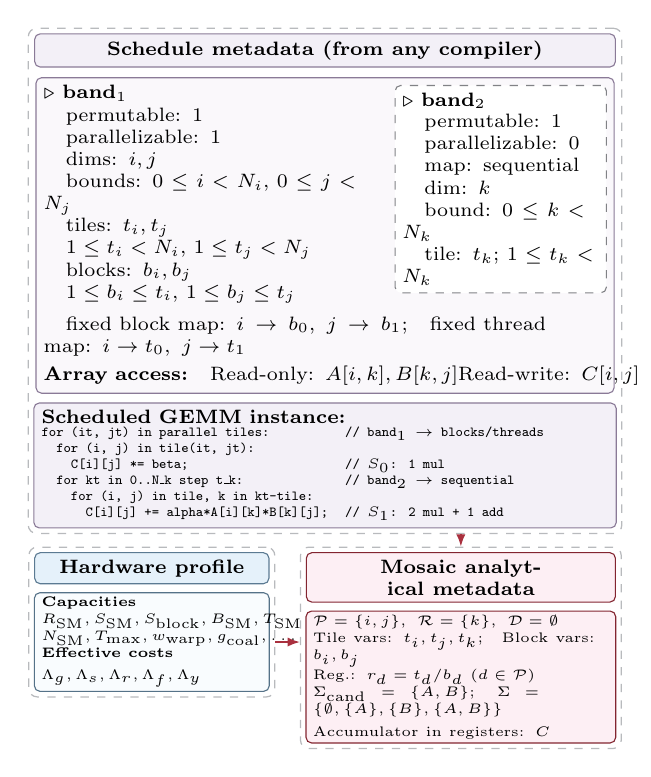
\begin{tikzpicture}[
  font=\scriptsize,
  box/.style={
    draw=color5!82!black,
    fill=white,
    rounded corners=2pt,
    inner sep=2.6pt,
    text width=#1,
    align=left
  },
  textonly/.style={
    text width=#1,
    align=left,
    inner sep=0pt
  },
  hdr/.style={
    draw=color5!82!black,
    rounded corners=2pt,
    inner sep=2.5pt,
    fill=color5!12,
    font=\scriptsize\bfseries,
    align=center
  },
  arr/.style={
    -{Latex[length=1.55mm]},
    line width=0.55pt,
    draw=color1!85!black
  },
  grpborder/.style={
    draw=color5!72,
    rounded corners=3pt,
    line width=0.45pt,
    dashed
  },
]

\node[
  hdr,
  text width=72mm,
  fill=color3!18,
  draw=color3!72!black
] (src_hdr) at (0,0)
  {Schedule metadata (from any compiler)};

\node[
  textonly=41mm,
  anchor=north west
] (bandone_text)
  at ([xshift=-35.8mm,yshift=-2.2mm]src_hdr.south)
{%
  \(\triangleright\) \textbf{band\(_1\)}\\
  \quad permutable: 1\\
  \quad parallelizable: 1\\
  \quad dims: \(i,j\)\\
  \quad bounds: \(0\le i<N_i\), \(0\le j<N_j\)\\
  \quad tiles: \(t_i,t_j\)\\
  \quad \(1\le t_i<N_i\), \(1\le t_j<N_j\)\\
  \quad blocks: \(b_i,b_j\)\\
  \quad \(1\le b_i\le t_i\), \(1\le b_j\le t_j\)
};

\node[
  box=25mm,
  dashed,
  anchor=north east
] (bandtwo_box)
  at ([xshift=35.8mm,yshift=-2.2mm]src_hdr.south)
{%
  \(\triangleright\) \textbf{band\(_2\)}\\[-0.2pt]
  \quad permutable: 1\\
  \quad parallelizable: 0\\
  \quad map: sequential\\
  \quad dim: \(k\)\\
  \quad bound: \(0\le k<N_k\)\\
  \quad tile: \(t_k\); \(1\le t_k<N_k\)
};

\node[
  textonly=68mm,
  anchor=north west
] (mapping_text)
  at ([xshift=0mm,yshift=-1.5mm]bandone_text.south west)
{%
  \quad fixed block map: \(i\to b_0,\ j\to b_1\);\quad
  fixed thread map: \(i\to t_0,\ j\to t_1\)
};

\node[
  textonly=68mm,
  anchor=north west
] (access_text)
  at ([xshift=0mm,yshift=-1.15mm]mapping_text.south west)
{%
  \makebox[\linewidth][l]{%
    \textbf{Array access:}\quad
    Read-only: \(A[i,k],B[k,j]\)\hfill
    Read-write: \(C[i,j]\)}
};

\begin{scope}[on background layer]
  \node[
    draw=color3!72!black,
    fill=color3!8,
    rounded corners=2pt,
    inner sep=2.6pt,
    fit=(bandone_text)(bandtwo_box)(mapping_text)(access_text)
  ] (loop_box) {};
\end{scope}

\node[
  box=72mm,
  draw=color3!72!black,
  fill=color3!18,
  anchor=north,
  inner xsep=2.8pt,
  inner ysep=2.5pt
] (code_box)
  at ([yshift=-1.1mm]loop_box.south)
{%
  \textbf{Scheduled GEMM instance:}\\[-0.2pt]
  {\ttfamily\fontsize{4.75pt}{5.75pt}\selectfont
  \begin{tabular}{@{}l@{\hspace{1.15em}}l@{}}
  for (it, jt) in parallel tiles:
    & // band$_1$ $\to$ blocks/threads\\
  \quad for (i, j) in tile(it, jt):
    & \\
  \qquad C[i][j] *= beta;
    & // $S_0$: 1 mul\\
  \quad for kt in 0..N\_k step t\_k:
    & // band$_2$ $\to$ sequential\\
  \qquad for (i, j) in tile, k in kt-tile:
    & \\
  \qquad\quad C[i][j] += alpha*A[i][k]*B[k][j];
    & // $S_1$: 2 mul + 1 add
  \end{tabular}}
};

\coordinate (lower_top)
  at ([yshift=-3.0mm]code_box.south);
\node[
  hdr,
  text width=28mm,
  fill=color4!24,
  draw=color4!62!black,
  anchor=north west
] (hw_hdr)
  at ([xshift=0mm]src_hdr.west |- lower_top)
  {Hardware profile};

\node[
  box=28mm,
  draw=color4!58!black,
  fill=color4!6,
  anchor=north,
  yshift=-1.0mm,
  minimum height=12.0mm,
  inner ysep=1.5pt
] (hw_box)
  at (hw_hdr.south)
{%
  {\fontsize{5.15pt}{6.15pt}\selectfont
  \textbf{Capacities}\\
  \(R_{\mathrm{SM}},
    S_{\mathrm{SM}},
    S_{\mathrm{block}},
    B_{\mathrm{SM}},
    T_{\mathrm{SM}}\)\\
  \(N_{\mathrm{SM}},
    T_{\max},
    w_{\mathrm{warp}},
    g_{\mathrm{coal}},
    \ldots\)\\
  \textbf{Effective costs}\\
  \(\Lambda_g,
    \Lambda_s,
    \Lambda_r,
    \Lambda_f,
    \Lambda_y\)}
};

\begin{scope}[on background layer]
  \node[
    grpborder,
    inner sep=1.8pt,
    fit=(hw_hdr)(hw_box)
  ] (hw_grp) {};
\end{scope}

\node[
  hdr,
  text width=37.5mm,
  fill=color2!24,
  draw=color1!66!black,
  anchor=north east
] (out_hdr)
  at ([xshift=0mm]src_hdr.east |- lower_top)
  {\name analytical metadata};

\node[
  box=37.5mm,
  draw=color1!66!black,
  fill=color2!24,
  anchor=north,
  yshift=-1.0mm,
  minimum height=12.0mm,
  inner ysep=1.5pt
] (out_box)
  at (out_hdr.south)
{%
  {\fontsize{5.15pt}{6.15pt}\selectfont
  \(\mathcal P=\{i,j\},\
    \mathcal R=\{k\},\
    \mathcal D=\emptyset\)\\
  Tile vars: \(t_i,t_j,t_k\);\quad
  Block vars: \(b_i,b_j\)\\
  Reg.: \(r_d=t_d/b_d\ (d\in\mathcal P)\)\\
  {\fontsize{4.55pt}{6.15pt}\selectfont
  \(\Sigma_{\mathrm{cand}}=\{A,B\};\quad
    \Sigma=\{\emptyset,\{A\},\{B\},\{A,B\}\}\)}\\
  Accumulator in registers: \(C\)}
};

\begin{scope}[on background layer]
  \node[
    grpborder,
    inner sep=1.8pt,
    fit=(out_hdr)(out_box)
  ] (out_grp) {};
\end{scope}

\begin{scope}[on background layer]
  \node[
    grpborder,
    inner sep=1.8pt,
    fit=(src_hdr)(loop_box)(code_box)
  ] (sched_grp) {};
\end{scope}

\coordinate (sched_arrow_start)
  at (out_grp.north |- sched_grp.south);

\draw[arr]
  (sched_arrow_start)
  -- (out_grp.north);

\coordinate (hw_exit)
  at (hw_grp.east |- hw_box.center);

\coordinate (hw_entry)
  at (out_grp.west |- hw_box.center);

\draw[arr]
  (hw_exit)
  -- (hw_entry);

\end{tikzpicture}%
}

\caption{
  GEMM metadata construction.
  Schedule metadata from the PPCG schedule tree, combined with a
  one-time hardware profile, yields the \name analytical metadata,
  with the dimension sets following \autoref{eq:dimension-roles}.
}
\label{fig:gemm-schedule-metadata}

\Description{
  A compact single-column flow diagram in which a rectangular
  schedule-metadata panel contains a GEMM schedule-tree instance,
  while a one-time hardware profile and the schedule metadata feed
  \name analytical metadata.
}

\end{wrapfigure}

In this example, the dimension sets defined in \autoref{eq:dimension-roles} give \(\mathcal{P}=\{i,j\}\), which creates \(\tile_i,\tile_j\) and \(b_i,b_j\); \(\mathcal{R}=\{k\}\), which creates \(\tile_k\) but no block dimension. The register-blocking factors \(\rblk_i=\tile_i/b_i\) and \(\rblk_j=\tile_j/b_j\) follow from these tile and block choices rather than entering as separate variables. The read-only operands give \(\Sigma_{\mathit{cand}}=\{A,B\}\), whose four binary-based placement scenarios change the modeled footprint, traffic, and resident-block bound used in \autoref{sec:model}.

\subsection{GPU Target Profiling}
\label{sec:gpu-target-profiling}

The target description combines hardware constants queried from the device with effective costs measured once per architecture and reused across all kernels for that target. The hardware constants, including SM count, warp size, resident block and thread limits, shared memory capacities, register-file size, and block-size limit (\autoref{tab:model-notation}), bound the resident-block count, occupancy, and feasible domain. The effective costs, the \(\Lambda\)-family constants of \autoref{tab:model-notation}, come from targeted microbenchmarks and enter the matching terms of \(T_{\mathit{block}}\). They serve relative ranking and analytical selection, not cycle-accurate prediction; the model captures the resource interactions that shape the execution space landscape and leaves backend scheduling, caching, and pipeline overlap as lower-level effects.

\begin{table}[tbp]
  \caption{Model notation.}
  \label{tab:model-notation}
  \centering
  \scriptsize
  \setlength{\tabcolsep}{4pt}
  \renewcommand{\arraystretch}{1.08}
  \begin{tabularx}{0.9\textwidth}{@{}
    >{\raggedright\arraybackslash}p{0.25\linewidth}
    >{\raggedright\arraybackslash}X
    @{}}
    \toprule
    \textbf{Symbol} & \textbf{Meaning} \\
    \midrule
    \multicolumn{2}{@{}l@{}}{\textbf{Optimization variables}} \\
    \addlinespace[1pt]
    \(\tile_d,\ b_d\) & Tile size and thread-block size for dimension~\(d\). \\
    \addlinespace[2pt]
    \midrule
    \addlinespace[2pt]
    \multicolumn{2}{@{}l@{}}{\textbf{Enumerated modeling state}} \\
    \addlinespace[1pt]
    \(S \in \Sigma\) & Abstract shared-memory placement scenario
                         (subset of \(\Sigma_{\mathit{cand}}\)). \\
    \addlinespace[2pt]
    \midrule
    \addlinespace[2pt]
    \multicolumn{2}{@{}l@{}}{\textbf{Architecture constants}\quad
      \textit{(queried or profiled once per GPU)}} \\
    \addlinespace[1pt]
    \(\Nsm,\Bsm,\Tsm,\Tmax\) &
      SM count; max resident blocks and threads per SM; max threads per block. \\
    \(\Ssm,\Sblock,\Rsm\) &
      Per-SM and per-block shared memory capacity; SM register-file size. \\
    \(\Lg,\Ls,\Lf,\Ly\) &
      Effective costs for global access, shared-memory access, FMA,
      and barrier synchronization. \\
    \(\Lr,\ \gcoal\) &
      Register-access cost; coalescing granularity for loads. \\
    \addlinespace[2pt]
    \midrule
    \addlinespace[2pt]
    \multicolumn{2}{@{}l@{}}{\textbf{Derived quantities}} \\
    \addlinespace[1pt]
    \(\rblk_d,\ \work\) & Register-blocking factor \(\rblk_d=\tile_d/b_d\) and
                           per-thread output count \(\work=\prod_{d\in\mathcal{P}}\rblk_d\). \\
    \(\phi_{\square}\) &
      Reads-per-FMA ratio for placement class
      \(\square\!\in\!\{\mathit{smem},\mathit{gmem}\}\);
      links register blocking to memory traffic in \(T_{\mathit{compute}}\). \\
    \(\rho_{\mathrm{reg}},\ \creg\) &
      Modeled register accesses per reduction-body evaluation;
      \(\creg=\rho_{\mathrm{reg}}\Lr\). \\
    \(\operatorname{smem}(\tvec;S),\ |A|_{\tvec}\) &
      Shared-memory footprint and operand tile footprint. \\
    \(K_{\mathit{outer}}\) &
      Cooperative load rounds \(\prod_{r\in\mathcal{R}}\lceil N_r/\tile_r\rceil\)
      over tiled reduction dimensions. \\
    \(bps,\ R_{\mathit{avail}},\ \hat{R}\) &
      Resident blocks per SM; available registers per thread \DIFaddbeginFL \revRthree{(32-bit slots)}\DIFaddendFL ;
      conservative register working-set estimate \DIFaddbeginFL \revRthree{(live values per thread)}\DIFaddendFL . \\
    \bottomrule
  \end{tabularx}
\end{table}

Each \(\Lambda\)-family constant of \autoref{tab:model-notation} is obtained from a dedicated CUDA microbenchmark: a pointer-chasing dependency chain larger than L2 for \(\Lg\), the corresponding shared-memory chain for \(\Ls\), dependent instruction chains for \(\Lr\) and \(\Lf\), and a barrier-only kernel for \(\Ly\). The resulting architecture-specific profile is generated once per GPU and reused across kernels and problem sizes.

% !TEX root =  mosaic.tex
\section{Analytical Modeling and Problem Solving}
\label{sec:model}

Given transformed metadata and target constants, \name selects tile sizes \(\tvec\) and thread-block dimensions \(\mathbf{b}\) while reasoning over abstract shared-memory placement scenarios \(S\) and accounting for occupancy and register pressure, inducing register-blocking factors \(\rblk_d=\tile_d/b_d\), footprints, resident blocks, waves, and register working sets; \autoref{tab:model-notation} summarizes the main notation. Recall from \autoref{eq:two-level} that the analytical comparison over \(S\) and \((\tvec,\mathbf{b})\) factorizes into outer placement-scenario enumeration and, for each fixed \(S\), an inner two-stage analytical selection. The primary inner objective is the quantized wave cost.
\begin{equation}
\min_{(\tvec,\mathbf{b})\in\mathcal{V}(S)}
T_{\mathit{block}}(\tvec,\mathbf{b};S)
\cdot
\left\lceil
\dfrac{N_{\mathit{blocks}}(\tvec)}
      {\Nsm \cdot bps(\tvec,\mathbf{b};S)}
\right\rceil,
\label{eq:model-summary}
\end{equation}
For a fixed modeled placement scenario \(S\), \autoref{eq:model-summary} minimizes over tile sizes and thread-block dimensions only. Here \(bps\) is the resident blocks per \sm (\autoref{eq:resident-blocks}) and \(T_{\mathit{block}}\) is the per-block cost (\autoref{eq:block-cost}); the ceiling is the scenario-dependent wave count. Thus, \autoref{eq:model-summary} is the primary objective of the per-scenario analytical selection in \autoref{eq:two-level}; the outer enumeration compares the primary scores first and uses the secondary score only to resolve ties. The feasible domain \(\mathcal{V}(S)\) enforces thread/block limits, minimum useful parallelism, shared-memory capacity, and register feasibility (\autoref{eq:feasible-domain}).

\subsection{Candidate Space}
\label{sec:abstraction}
\label{sec:placement}

From the metadata of \autoref{sec:metadata}, each loop dimension is labeled according to its role in the transformed schedule. Parallel dimensions are those the upstream compiler has determined can legally execute across independent thread blocks and threads; reduction dimensions are those absent from all write footprints, meaning their iterations produce partial results that must be accumulated; serial dimensions are those that are neither parallel nor reduction and must execute sequentially within each thread. Formally:
\begin{equation}
\begin{aligned}
\mathcal{P}
&= \{d \mid \mathit{parallelizable}[d] = 1\},\\
\mathcal{R}
&= \{d \notin \mathcal{P}
    \mid d \notin \dim(A)\ \text{for every written array } A\},\\
\mathcal{D}
&= \{d \mid d\notin\mathcal{P},\ d\notin\mathcal{R}\}.
\end{aligned}
\label{eq:dimension-roles}
\end{equation}
\(\mathit{parallelizable}[d]=1\) denotes a dimension that can legally execute in parallel; for polyhedral schedules this includes coincident dimensions with no carried dependence, and TVM axes bound to CUDA block or thread indices are treated analogously. Reduction axes populate \(\mathcal{R}\), and serial dimensions remain untiled. Serial dimensions \(\mathcal{D}\) are those belonging to neither \(\mathcal{P}\) nor \(\mathcal{R}\); they remain at their full loop extents, are not assigned tile or block variables, and do not contribute to the candidate generation of \autoref{eq:tile-candidates}. For GEMM, \(\mathcal{D}=\emptyset\).

Under the compiler-provided mapping, parallel dimensions correspond to thread and block indices, while reduction dimensions contribute only to per-output work \(K_{\mathit{total}}\). The reduction work per output element is a compile-time constant independent of any tile choice:
\begin{equation}
K_{\mathit{total}} = \prod_{r \in \mathcal{R}} N_r.
\label{eq:reduction-work}
\end{equation}

\name builds a discrete tile candidate set from powers of two and exact divisors:
\begin{equation}
C_d
= \{2^k \mid 2^k < N_d\}
  \cup \{v \mid v \text{ divides } N_d\}.
\label{eq:tile-candidates}
\end{equation}
\name uses powers of two and exact divisors to keep the analytical candidate space bounded. Powers of two provide hardware-aligned choices, while exact divisors avoid boundary remainders. We do not assume that other tile sizes are inherently inferior; \autoref{subsec:bounded-ppcg-sweep} evaluates a broader empirical space including unaligned and non-divisor configurations to quantify the performance opportunity outside this analytical candidate set. For each \(\tile_d\in C_d\), block candidates are restricted to divisors of \(\tile_d\), keeping
\(\rblk_d=\tile_d/b_d\) integral; hardware limits are imposed later.

Each array is assigned a memory space from its read/write polarity
(\autoref{tab:placement-rules}). Read-only operands form
\(\Sigma_{\mathit{cand}}\), and \name enumerates
\(\Sigma=2^{\Sigma_{\mathit{cand}}}\) during solving of
\autoref{eq:two-level}. Accumulators and ordinary write-only references are
excluded, keeping the placement-scenario space small.

Equivalently, the joint execution-space candidate set is \(\prod_{d\in\mathcal{P}\cup\mathcal{R}} C_d \times \Sigma\), with each \(\tile_d\in C_d\) paired with divisor choices for admissible block dimensions; \(\mathcal{V}(S)\) then filters this product to legal configurations for the objective of \autoref{eq:two-level}. This candidate space contains tile sizes, thread-block dimensions under the compiler-provided mapping, and abstract modeled placement scenarios; it contains no schedule, mapping structure, or execution-order variables.

Following the placement rules in \autoref{tab:placement-rules}, for a fixed \(S\), let \(\mathcal{A}_{\mathit{smem}}=S\) and \(\mathcal{A}_{\mathit{gmem}}=\Sigma_{\mathit{cand}}\setminus S\). With \(\work=\prod_{d\in\mathcal{P}}\rblk_d\) outputs per thread, the induced resource quantities used by the constraints and cost model are the shared memory footprint \(\operatorname{smem}(\tvec;S)\), the read counts \(R^{\mathit{smem}}_{\mathit{in}}\) and \(R^{\mathit{gmem}}_{\mathit{in}}\), and the register working set \(\hat{R}\). The per-reduction-step read count and its normalized ratio are
\begin{equation}
\begin{aligned}
R^{\square}_{\mathit{in}}
&=\sum_{A \in \mathcal{A}_{\square}}
  \prod_{d \in \dim(A) \cap \mathcal{P}} \rblk_d,\\[0.6ex]
\phi_{\square}
&=\dfrac{R^{\square}_{\mathit{in}}}{\work}
 =\sum_{A \in \mathcal{A}_{\square}}
  \prod_{d \in \mathcal{P} \setminus \dim(A)} \rblk_d^{-1},
\qquad \square \in \{\mathit{smem},\mathit{gmem}\}.
\end{aligned}
\label{eq:read-ratios}
\end{equation}

For the GEMM example with both operands staged (\(\mathcal{P}=\{i,j\}\), \(\mathcal{R}=\{k\}\), \(\Sigma_{\mathit{cand}}=\{A,B\}\); \autoref{fig:gemm-schedule-metadata}), \autoref{eq:read-ratios} gives \(\work=\rblk_i\rblk_j\) outputs per thread and \(\phi_{\mathit{smem}}=\rblk_i^{-1}+\rblk_j^{-1}\).

\subsection{Feasibility Constraints}
\label{sec:constraints}
\label{sec:register-filter}

The inner feasible domain \(\mathcal{V}(S)\) is the set of tile/block choices that, for a fixed modeled placement scenario \(S\), satisfy every launch and resource constraint; it is the domain over which the inner objective (\autoref{eq:model-summary}) is minimized, after which the outer loop compares the optima across modeled scenarios (\autoref{eq:two-level}). It collects launch limits and pruning rules:
\begin{equation}
\begin{gathered}
\mathcal{V}(S)
= \{(\tvec,\mathbf{b}) \mid \text{C1--C4 hold}\},\\[0.6ex]
\begin{array}{@{}l@{\qquad}l@{}}
\text{C1: } \displaystyle \prod_{d\in\mathcal{P}} b_d \le \Tmax
&
\text{C2: } \displaystyle \prod_{d\in\mathcal{P}} b_d \ge \Wwarp\\[0.7ex]
\text{C3: } \operatorname{smem}(\tvec;S)\le \Sblock
&
\text{C4: } \hat{R}\le R_{\mathit{avail}}.
\end{array}
\end{gathered}
\label{eq:feasible-domain}
\end{equation}
C1 and C2 enforce block-size legality and useful parallelism; C3 bounds placement-dependent shared memory; C4 is the conservative register filter.

The register filter breaks the occupancy and register circular dependence by ordering the quantities in one direction; the symbols used below are summarized in \autoref{tab:model-notation}. First, \name ignores the register constraint and computes a pre-register resident-block bound from the block limit, thread limit, and shared memory usage. This gives \(bps\). Second, \(bps\) and the number of threads per block determine the available register budget per thread, \(R_{\mathit{avail}}\). Third, a conservative working set estimate \(\hat{R}\) is checked against that budget:
\begingroup
\renewcommand{\arraystretch}{1.12}
\begin{equation}
\begin{aligned}
bps
&= \min\left(
   \Bsm,
   \left\lfloor \dfrac{\Tsm}{\prod_{d\in\mathcal{P}} b_d} \right\rfloor,
   \left\lfloor
   \dfrac{\Ssm}{\operatorname{smem}(\tvec;S)}
   \right\rfloor
   \right),
&\qquad
R_{\mathit{avail}}
&= \left\lfloor
   \dfrac{\Rsm}{bps \cdot \prod_{d\in\mathcal{P}} b_d}
   \right\rfloor,\\[1.5ex]
\hat{R}
&= \work + R^{\mathit{live}}_{\mathit{in}} + \Czero,
\qquad
R^{\mathit{live}}_{\mathit{in}}
= R^{\mathit{smem}}_{\mathit{in}} + R^{\mathit{gmem}}_{\mathit{in}}.
\end{aligned}
\label{eq:resident-blocks}
\end{equation}
\endgroup
When \(\operatorname{smem}(\tvec;S)=0\), the shared memory ceiling in \(bps\) is omitted. The offset \(\Czero\) counts the control and addressing registers that stay live throughout the kernel, namely the reduction loop counters and the shared and global base pointers. Its value is fixed once the loop nest and modeled placement scenario are known and does not vary with the tile or block choice, so the solver treats it as a constant. \(\hat R\) is a conservative register lower bound because the counted values are simultaneously live. \DIFaddbegin \revRthree{$R_{\mathit{avail}}$ counts 32-bit slots and depends on precision only through $bps$, which the byte-sized shared-memory footprint can limit. $\hat{R}$ instead counts values; since an FP32 value occupies one slot and an FP64 value two, $\hat{R}$ remains a lower bound at either precision, though a looser one in FP64.} \DIFaddend Thus, \(\hat R > R_{\rm avail}\) is sufficient to reject a configuration, whereas \(\hat R \le R_{\rm avail}\) only means that register infeasibility has not been established. C4 is therefore a one-sided pruning test rather than a predictor of backend allocation: violating the bound means that the modeled working-set lower bound already exceeds the register budget implied by the current residency estimate, while satisfying C4 does not guarantee spill-free backend allocation. \autoref{sec:eval} validates this distinction against post-compilation register behavior. \DIFaddbegin \revRthree{C4 is evaluated at the pre-register residency $bps$ at which Eq.~\eqref{eq:model-summary} counts waves; a configuration with $\hat R > R_{\mathit{avail}}$ cannot reach $bps$, and scoring it there would underestimate its wave count. C4 may therefore exclude a configuration that runs efficiently at lower residency when registers limit residency; \autoref{sec:eval} measures this effect.}
\DIFaddend

For the GEMM feasibility example with modeled scenario \(S=\{A,B\}\), tile sizes
\(\tile_i,\tile_j,\tile_k\), and
block dimensions \(b_i,b_j\), C1 requires \(b_i b_j\le \Tmax\) and C2
requires \(b_i b_j\ge \Wwarp\). C3 requires the shared memory footprint
\[
\operatorname{smem}(\tvec;\{A,B\}) =
\operatorname{sizeof}(\mathit{dtype})\cdot(\tile_i\tile_k+\tile_k\tile_j)
\le \Sblock,
\]
where the first term is the \(A\)-tile of size \(\tile_i\times\tile_k\) and the
second is the \(B\)-tile of size \(\tile_k\times\tile_j\). The pre-register
resident-block bound is
\[
bps=\min\left(\Bsm,
\left\lfloor \frac{\Tsm}{b_i b_j}\right\rfloor,
\left\lfloor
\frac{\Ssm}{\operatorname{sizeof}(f)\cdot(\tile_i\tile_k+\tile_k\tile_j)}
\right\rfloor\right).
\]
The corresponding register budget per thread is
\[
R_{\mathit{avail}}=\left\lfloor
\frac{\Rsm}{bps\cdot b_i b_j}\right\rfloor.
\]
The simultaneously live values inside the inner FMA loop are the \(\work=\rblk_i\rblk_j\) accumulators, \(\rblk_i\) values from \(A\), \(\rblk_j\) values from \(B\), and the fixed control/addressing offset \(\Czero\). For GEMM, the single reduction loop contributes one tile-loop and one point-loop counter, and staging adds one shared and one global base pointer, giving \(\Czero=4\). Hence \(\hat{R}=\rblk_i\rblk_j+\rblk_i+\rblk_j+\Czero\), and C4 rejects the configuration when
\[
\rblk_i\rblk_j+\rblk_i+\rblk_j+\Czero >
\left\lfloor \frac{\Rsm}{bps\cdot b_i b_j}\right\rfloor.
\]
Since \(bps\) depends on the shared memory footprint, C4 couples tile, block, and register decisions and must be resolved jointly by the MILP.

\subsection{Cost Model and Objective}
\label{sec:cost}
\label{sec:outer-product-optimality}
\label{sec:kernel-specialization}

With feasibility fixed, \name ranks the surviving configurations by modeled time. For one modeled placement scenario and configuration, the time is the per-block cost scaled by the number of residency waves:
\begin{equation}
\begin{aligned}
T_{\mathit{total}}
&=T_{\mathit{block}}
  \left\lceil\frac{N_{\mathit{blocks}}}{C_{\mathit{blocks}}}\right\rceil,\\[0.6ex]
N_{\mathit{blocks}}
&=\prod_{d\in\mathcal{P}}\left\lceil\frac{N_d}{\tile_d}\right\rceil,
\qquad C_{\mathit{blocks}}=\Nsm\cdot bps.
\end{aligned}
\label{eq:discrete-wave}
\end{equation}
This modeled total time is the quantized Stage-1 cost denoted by \(F(\tvec,\mathbf{b};S)\) in \autoref{eq:stage-one}.
\(N_{\mathit{blocks}}\) is the grid size and \(C_{\mathit{blocks}}\) is the number of blocks resident across all SMs, so the ceiling counts how many waves the grid takes. This ceiling is an integer step function, so a smaller per-block cost can still raise \(T_{\mathit{total}}\) once it forces one extra wave. These step boundaries, not any smooth trend, produce the irregular landscape of \autoref{fig:motivation-landscape}, and a useful objective must track them.

The per-block cost decomposes as
\begin{equation}
T_{\mathit{block}}
= T_{\mathit{init}} + T_{\mathit{load}} + T_{\mathit{compute}} +
   T_{\mathit{write}} + T_{\mathit{sync}}.
\label{eq:block-cost}
\end{equation}
charging output initialization, cooperative loads, arithmetic, global writes, and barriers. With \(\work=\prod_{d\in\mathcal{P}}\rblk_d\) outputs per thread and \(K_{\mathit{outer}}=\prod_{r\in\mathcal{R}}\lceil N_r/\tile_r\rceil\) staging rounds,
\begin{itemize}
  \item \(T_{\mathit{init}} = \work \cdot \Lr\), one accumulator-register initialization per output, charged at the register-access cost \(\Lr\) (Tab.~\ref{tab:model-notation}); this is the per-output accumulator setup, distinct from the arithmetic of \(s_{\mathit{out}}\).
  \item \(T_{\mathit{load}}\) is the coalesced load of each staged tile:
  \[
  T_{\mathit{load}} = K_{\mathit{outer}}\sum_{A \in \mathcal{A}_{\mathit{smem}}}
  \frac{\lceil |A|_{\tvec} / \gcoal \rceil}{\min(\prod_{d \in \mathcal{P}} b_d,\lceil |A|_{\tvec} / \gcoal \rceil)}
  \Lg,
  \]
  where \(|A|_{\tvec}\) is the tile footprint and \(\gcoal\) is the coalescing granularity.
  \item Compute cost is
  \begin{equation}
	  \begin{aligned}
	  T_{\mathit{compute}} &= \work \cdot
	    \left(n_{\mathit{op}}(s_{\mathit{out}})\Lf
	    + K_{\mathit{total}}\cdot\cfma\right),\\[1ex]
	  \cfma &= n_{\mathit{op}}(s_{\mathit{red}})\Lf
	  + \phi_{\mathit{smem}}\Ls
	  + \phi_{\mathit{gmem}}\Lg
	  + \creg.
	  \end{aligned}
	  \label{eq:fma-cost}
	  \end{equation}
	  The residual register term is \(\creg=\rho_{\mathrm{reg}}\Lr\), where \(\rho_{\mathrm{reg}}\) is the modeled number of register accesses associated with one reduction-body evaluation, derived from the statement metadata. The coefficient is independent of the modeled placement scenario, while its total contribution scales with the per-thread work through \autoref{eq:fma-cost}. Here \(n_{\mathit{op}}(s)\) is the operation count of statement \(s\) in the statement metadata, \(s_{\mathit{out}}\) the statement that runs once per output, and \(s_{\mathit{red}}\) the reduction-body statement that runs \(K_{\mathit{total}}\) times; the counts add when a group holds several statements. The \(n_{\mathit{op}}(s_{\mathit{out}})\) work is charged once per output with no \(K_{\mathit{total}}\) factor, while the reduction body carries \(K_{\mathit{total}}\), and the factor \(\work\) scales both to the thread's output count. Both remain terms of \(T_{\mathit{compute}}\) and hence of the per-block cost \(T_{\mathit{block}}\) in \autoref{eq:block-cost}.
  \item \(T_{\mathit{write}}=\work\cdot \Lg\), charging one global write per output.
  \item \(T_{\mathit{sync}}=2K_{\mathit{outer}}\Ly\cdot\mathbf{1}[\mathcal{A}_{\mathit{smem}}\ne\emptyset]\), charging two barriers per staging round.
\end{itemize}

The link from modeled placement-scenario reasoning to register blocking is the shared-read-per-FMA ratio \(\phi_{\square}\) of \autoref{eq:read-ratios}, the operand reads of class \(\square\in\{\mathit{smem},\mathit{gmem}\}\) per reduction step divided by the per-thread work \(\work\). A lower \(\phi_{\mathit{smem}}\) spreads each staged read over more arithmetic and lowers the \(\cfma\) term above, as long as the footprint still satisfies C3. For an outer-product contraction the staged reads of each operand depend on a single register factor, so \(\work\phi_{\mathit{smem}}\) is a sum of \(|\mathcal{P}|\) factors whose product is fixed at \(\work\). The arithmetic-mean-geometric-mean (AM-GM) inequality states that a sum of nonnegative terms with a fixed product is smallest when the terms are equal; applying it gives
\[
\work\phi_{\mathit{smem}} \ge |\mathcal{P}| \cdot \work^{1/|\mathcal{P}|},
\quad \text{with equality at } \rblk_d=\work^{1/|\mathcal{P}|}.
\]
Balanced register blocking is therefore an analytical optimum rather than an imposed rule. For GEMM, \(|\mathcal{P}|=2\) and \(\work\phi_{\mathit{smem}}=\rblk_i+\rblk_j\), so the optimum is \(\rblk_i=\rblk_j=\sqrt{\work}\).

The same lever behaves differently by kernel class, and \name selects the form from the access footprints. Symmetric contractions admit the balanced optimum above. Asymmetric or broadcast reductions such as \texttt{atax} in PolyBench~\cite{polybench} give \(\work\phi_{\mathit{smem}}=\rblk_i+1\) with no interior optimum, so the MILP picks the best point directly. Stencils such as Jacobi-2D~\cite{polybench} reuse data through halo overlap rather than a broadcast dimension. For one staged stencil operand, or several with the same halo, and with \(h_d\) the single-sided halo width,
\begin{equation}
\begin{aligned}
R^{\mathit{smem}}_{\mathit{in}}
\approx \prod_{d\in\mathcal{P}}(\rblk_d+2h_d),
\qquad
\phi_{\mathit{smem}}
= \prod_{d\in\mathcal{P}}\left(1+\frac{2h_d}{\rblk_d}\right).
\end{aligned}
\label{eq:stencil-halo}
\end{equation}
A larger register tile drives \(\phi_{\mathit{smem}}\) toward one and can cut waves, while C3 still bounds it through the halo-inflated footprint. With several arrays and unequal halos the footprint becomes \(\sum_A\prod_d(\rblk_d+2h_{A,d})\), a product of sums rather than a single product, so the equal-term optimum no longer applies and \name evaluates the full objective over all candidates.

For GEMM with \(S=\{A,B\}\), the terms instantiate directly in the tile and block variables. With \(\work=\rblk_i\rblk_j\), \(K_{\mathit{total}}=N_k\), \(K_{\mathit{outer}}=\lceil N_k/\tile_k\rceil\), footprints \(|A|_{\tvec}=\tile_i\tile_k\) and \(|B|_{\tvec}=\tile_k\tile_j\), and \(\phi_{\mathit{gmem}}=0\),
\begingroup
\renewcommand{\arraystretch}{1.18}
\[
\begin{array}{@{}l@{\;}l@{}}
T_{\mathit{init}}
&= \rblk_i\rblk_j\Lr,\\[1ex]
T_{\mathit{load}}
&= \left\lceil\frac{N_k}{\tile_k}\right\rceil
   \sum_{X\in\{A,B\}}
   \frac{\lceil |X|_{\tvec}/\gcoal\rceil}{\min(b_i b_j,\lceil |X|_{\tvec}/\gcoal\rceil)}
   \Lg,\\[1ex]
T_{\mathit{compute}}
&= \rblk_i\rblk_j
   \left(
   \Lf
   + N_k\left(3\Lf+(\rblk_i^{-1}+\rblk_j^{-1})\Ls+\creg\right)
   \right),\\[1ex]
T_{\mathit{write}}
&= \rblk_i\rblk_j\Lg,\\[1ex]
T_{\mathit{sync}}
&= 2\left\lceil\frac{N_k}{\tile_k}\right\rceil\Ly.
\end{array}
\]
\endgroup
For GEMM, \(s_{\mathit{out}}=S_0\) and \(s_{\mathit{red}}=S_1\). The scaling statement \(S_0\) contributes \(n_{\mathit{op}}(S_0)=1\) once per output, the leading \(\rblk_i\rblk_j\Lf\) term of \(T_{\mathit{compute}}\) that carries no \(N_k\) factor, and the update statement \(S_1\) contributes \(n_{\mathit{op}}(S_1)=3\) per reduction step, the \(\rblk_i\rblk_jN_k\) term. Both stay inside \(T_{\mathit{compute}}\) and therefore inside \(T_{\mathit{block}}\); \(T_{\mathit{init}}\) is separate, charging only the accumulator-register initialization (one register write per output at \(\Lr\)), not the \(\beta\)-scaling arithmetic of \(S_0\), which is already counted as \(s_{\mathit{out}}\) in \(T_{\mathit{compute}}\). Multiplying \(T_{\mathit{block}}\) by the wave ceiling of \autoref{eq:discrete-wave} adds the discontinuity seen in \autoref{fig:motivation-landscape}.

\subsection{Solving Procedure}
\label{sec:solver}
\label{sec:two-stage-solver}

\autoref{eq:two-level}, \autoref{eq:model-summary}, and \autoref{eq:block-cost} form one hierarchy, not three independent objectives. \autoref{eq:block-cost} gives the per-block cost \(T_{\mathit{block}}\), \autoref{eq:model-summary} multiplies it by the integer wave count to form the quantized primary objective for a fixed modeled scenario, and \autoref{eq:two-level} compares the primary per-scenario scores before using the secondary scores to resolve ties. \name evaluates \autoref{eq:two-level} by enumerating placement scenarios and applying the two-stage analytical selection below to each \DIFaddbegin \revRtwo{(Algorithm~\ref{alg:mosaic})}\DIFaddend , with \(T_{\mathit{block}}\) supplied by \autoref{eq:block-cost}. For the Stage-1 MILP encoding, for each \(S\in\Sigma\) and dimension \(d\), let
\(C_d=\{(v_{d,1},u_{d,1}),\ldots,(v_{d,K_d},u_{d,K_d})\}\) be the discrete
\((\tile_d,b_d)\) pairs. Introduce a one-hot indicator:
\[
z_{d,k}\in\{0,1\},
\qquad \sum_{k=1}^{K_d}z_{d,k}=1,
\qquad \tile_d=\sum_k v_{d,k}z_{d,k},
\qquad b_d=\sum_k u_{d,k}z_{d,k}.
\]
Products of \(z\)-variables in footprints and wave counts are linearized with
auxiliary variables \(y\):
\[
y\le z_{d_1,k_1},
\qquad y\le z_{d_2,k_2},
\qquad y\ge z_{d_1,k_1}+z_{d_2,k_2}-1.
\]
The same technique handles nonlinear terms in C3 and C4.

The outer loop explicitly enumerates only the modeled placement-scenario set \(\Sigma\). For each fixed \(S\), the discrete tile/block choices are encoded by the one-hot variables above and the Stage-1 MILP is solved under C1--C4 to obtain \(F^*(S)\). Stage 2 then considers only the discrete assignments tied at the Stage-1 optimum, keeping placement-scenario enumeration and tile/block optimization as separate levels of the solving procedure.

\DIFaddbegin \begin{algorithm}[tbp]
\small
\ifrevmarkup\captionsetup{labelfont+={color=revRtwo}}\fi
\caption{\revRtwo{Two-stage analytical selection in \name}}\label{alg:mosaic}
\begin{revRtwoblock}
\begin{algorithmic}[1]
\Require \DIFadd{Schedule metadata \(\mathcal{M}\), target profile \(\mathcal{H}\)
}\Ensure \DIFadd{Tile sizes \(\tvec^*\), thread-block dimensions \(\mathbf b^*\)
}\State \DIFadd{Partition the dimensions into \(\mathcal P,\mathcal R,\mathcal D\) using Eq.~}\eqref{eq:dimension-roles}\DIFadd{. Build tile candidates by Eq.~}\eqref{eq:tile-candidates}\DIFadd{, pairing tiles with block extents on mapped parallel axes.
}\ForAll{placement scenarios \(S\subseteq\Sigmacand\)}
  \State \textbf{\DIFadd{Stage 1.}} \DIFadd{Minimize \(F=T_{\mathit{block}}\lceil N_{\mathit{blocks}}/C_{\mathit{blocks}}\rceil\) subject to C1--C4. Retain \(F^*(S)\) and all tied discrete optima \(\mathcal V_1(S)\).
  }\State \textbf{\DIFadd{Stage 2.}} \DIFadd{Minimize \(\Phi=T_{\mathit{block}}N_{\mathit{blocks}}/C_{\mathit{blocks}}\) over \(\mathcal V_1(S)\). Retain \((\tvec_S^*,\mathbf b_S^*)\) and \(\Phi^*(S)\).
}\EndFor
\State \DIFadd{\(S^*\gets\arg\min_S^{\mathrm{lex}}\,(F^*(S),\Phi^*(S))\)
}\State \Return \DIFadd{\((\tvec_{S^*}^*,\mathbf b_{S^*}^*)\) }\Comment{The backend does not receive \(S^*\).}
\end{algorithmic}
\end{revRtwoblock}
\end{algorithm}

\DIFaddend As previewed at \autoref{eq:two-level}, the inner solve is a two-stage analytical selection. For a fixed modeled placement scenario \(S\), Stage 1 minimizes the quantized wave cost over the feasible discrete domain:
\begin{equation}
\begin{aligned}
F(\tvec,\mathbf{b};S)
&=T_{\mathit{block}}(\tvec,\mathbf{b};S)
  \left\lceil
  \frac{N_{\mathit{blocks}}(\tvec)}{C_{\mathit{blocks}}(\tvec,\mathbf{b};S)}
  \right\rceil,\\
F^*(S)
&=\min_{(\tvec,\mathbf{b})\in\mathcal{V}(S)}
  F(\tvec,\mathbf{b};S),\\
\mathcal{V}_1(S)
&=\left\{(\tvec,\mathbf{b})\in\mathcal{V}(S)
  \mid F(\tvec,\mathbf{b};S)=F^*(S)\right\}.
\end{aligned}
\label{eq:stage-one}
\end{equation}
Thus, \(\mathcal{V}_1(S)\) contains all feasible discrete tile/block configurations tied for the Stage-1 optimum.

Stage 2 evaluates the cost with the wave ceiling removed only over \(\mathcal{V}_1(S)\):
\begin{equation}
\Phi(\tvec,\mathbf{b};S)
=T_{\mathit{block}}(\tvec,\mathbf{b};S)
 \frac{N_{\mathit{blocks}}(\tvec)}{C_{\mathit{blocks}}(\tvec,\mathbf{b};S)},
\label{eq:relaxed-cost}
\end{equation}
\begin{equation}
\begin{aligned}
(\tvec_S^*,\mathbf{b}_S^*)
&\in \mathop{\arg\min}_{(\tvec,\mathbf{b})\in\mathcal{V}_1(S)}
 \Phi(\tvec,\mathbf{b};S),\\
\Phi^*(S)
&=\Phi(\tvec_S^*,\mathbf{b}_S^*;S).
\end{aligned}
\label{eq:stage-two}
\end{equation}
Stage 2 does not re-solve in a continuous tile/block space: \(\tvec\) and \(\mathbf{b}\) always come from the legal discrete Stage-1 optimum set. Only the wave count is relaxed, from \(\lceil N_{\mathit{blocks}}/C_{\mathit{blocks}}\rceil\) to \(N_{\mathit{blocks}}/C_{\mathit{blocks}}\). The relaxed-cost tie-break therefore produces neither fractional tile/block values nor a configuration that sacrifices the Stage-1 quantized optimum. This implements a lexicographic tie-break: the quantized Stage-1 objective has strict priority, and \(\Phi\) is consulted only among configurations tied at the Stage-1 optimum.

Wave quantization can create plateaus in which multiple discrete configurations have the same Stage-1 objective. Stage 2 evaluates the corresponding unquantized cost only over the Stage-1 optimal set, recovering ordering information within a quantization plateau while preserving the quantized optimum. The integer ceiling captures the actual discrete wave behavior, while the relaxed ratio provides finer ranking information only when the primary objective is tied.

Once the two-stage selection finishes for every \(S\in\Sigma\), the outer enumeration applies the scenario comparison of \autoref{eq:two-level}, equivalently written in lexicographic form as
\begin{equation}
\begin{aligned}
S^*
&\in \mathop{\arg\min}_{S\in\Sigma}^{\mathrm{lex}}
   \bigl(F^*(S),\Phi^*(S)\bigr),\\
(\tvec^*,\mathbf{b}^*)
&=(\tvec_{S^*}^*,\mathbf{b}_{S^*}^*).
\end{aligned}
\label{eq:outer-selection}
\end{equation}
Modeled placement scenarios are therefore compared first by \(F^*(S)\), with \(\Phi^*(S)\) used only when the primary costs tie. For programs representable by the metadata of \autoref{sec:metadata}, the scenario set stays small.

The construction of \autoref{sec:abstraction} through \autoref{sec:solver} is kernel-independent: dimension classification, candidate generation, feasibility, and the wave objective take the same form for every class. Only the closed form of \(\phi_{\mathit{smem}}\) varies with the reuse pattern, the omitted-dimension form for contractions versus the halo-amortization form of \autoref{eq:stencil-halo} for stencils, with \name selecting between them from the access footprints; in the stencil case \(\phi_{\mathit{smem}}\) becomes a product of sums, so the interior AM-GM optimum no longer applies and \name evaluates all candidates.

Tracing this end to end on the running GEMM example (\autoref{sec:metadata}\textendash\autoref{sec:solver}): profiled hardware constants and extracted schedule metadata instantiate \(\mathcal{V}(S)\) and the quantized objective for every \(S\in\Sigma\); the two-stage selection returns \((\tvec^*,\mathbf{b}^*,S^*)\), where \(S^*\) remains modeled analytical state, and only \(\tvec^*\) and \(\mathbf{b}^*\) are written back as backend configuration, with no candidate kernel generated or evaluated.

% !TEX root =  mosaic.tex
\section{Evaluation}
\label{sec:eval}

Our cross-generation PolyBench evaluation uses three generations of NVIDIA GPUs whose hardware and software platforms are summarized in \autoref{tab:platforms}. The architectural parameters required by the cost model, including memory capacities, execution limits, and the profiled \(\Lambda\)-family and \(c\) constants described in \autoref{sec:gpu-target-profiling} and used by \autoref{sec:cost}, are gathered once per GPU through the target description of \autoref{sec:overview} and reused across all kernels. \DIFaddbegin \revRone{Table~\ref{tab:platforms} also lists the H800 (Hopper), on which we additionally evaluate all 25 kernels after regenerating only the target profile (\autoref{subsec:polybench}).}
\DIFaddend

\begin{table}[tbp]
  \centering
  \caption{Experimental platforms. All experiments use CUDA's default \SI{48}{KiB} per-block shared-memory limit without opt-in.}
  \label{tab:platforms}
  \scriptsize
  \begin{adjustbox}{max width=\linewidth}
  \DIFdelbeginFL %DIFDELCMD < \begin{tabular}{lccc}
%DIFDELCMD <     %%%
\DIFdelendFL \DIFaddbeginFL \begin{tabular}{lcccc}
    \DIFaddendFL \toprule
     & RTX 4090 & A100 & V100 \DIFaddbeginFL & \revRone{H800} \DIFaddendFL \\
    \midrule
    Architecture & Ada & Ampere & Volta \DIFaddbeginFL & \revRone{Hopper} \DIFaddendFL \\
    SM count & 128 & 108 & 80 \DIFaddbeginFL & \revRone{132} \DIFaddendFL \\
    L1 / L2 cache & \SI{128}{KiB} / \SI{72}{MiB} & \SI{192}{KiB} / \SI{40}{MiB} & \SI{128}{KiB} / \SI{6}{MiB} \DIFaddbeginFL & \revRone{\SI{256}{KiB} / \SI{50}{MiB}} \DIFaddendFL \\
    Shared mem.\ per block / SM & \SI{48}{KiB} / \SI{100}{KiB} & \SI{48}{KiB} / \SI{164}{KiB} & \SI{48}{KiB} / \SI{96}{KiB} \DIFaddbeginFL & \revRone{\SI{48}{KiB} / \SI{228}{KiB}} \DIFaddendFL \\
    Registers per SM & 65536 & 65536 & 65536 \DIFaddbeginFL & \revRone{65536} \DIFaddendFL \\
    Global memory & \SI{48}{GiB} & \SI{80}{GiB} & \SI{32}{GiB} \DIFaddbeginFL & \revRone{\SI{80}{GiB}} \DIFaddendFL \\
    OS & Ubuntu 22.04 & Ubuntu 22.04 & Ubuntu 22.04 \DIFaddbeginFL & \revRone{Ubuntu 22.04} \DIFaddendFL \\
    CUDA / Compiler & 12.2 / NVCC 12.2.91 & 12.2 / NVCC 12.2.91 & 12.2 / NVCC 12.2.91 \DIFaddbeginFL & \revRone{12.8 / NVCC 12.8.93} \DIFaddendFL \\
    \bottomrule
  \end{tabular}
  \end{adjustbox}
\end{table}

All PolyBench/C 4.2.1~\cite{polybench} measurements, in \autoref{tab:benchmark} and in the bounded PPCG sweep of \autoref{subsec:bounded-ppcg-sweep}, use the official \texttt{EXTRALARGE} problem sizes and FP64 precision. The precision follows each backend's own convention rather than being imposed by \name: the PPCG path is FP64, matching the PolyBench/C and PolyNN~\cite{polynn} sources, while the TVM path is FP32, matching MetaSchedule's default tensor type; \autoref{tab:vendor-comparison} reports both FP64 and FP32/TF32 for the same GEMM shapes. \DIFdelbegin \DIFdel{Because the cost model reasons about tile footprints, register working sets, and traffic in bytes rather than in elements, the }\DIFdelend \DIFaddbegin \revRthree{Shared-memory footprints and traffic are measured in bytes. The} \DIFaddend element width enters only through the array element size of \autoref{sec:compile-time-metadata}, so the same formulation drives both regimes without retuning; the FP64 gains over PPCG and the FP32 gains over MetaSchedule reported below are evidence that this holds in practice. \name selects configurations for a given precision and does not change it. We verified output correctness for every measured configuration.

The same timing protocol is used for PolyBench, the bounded PPCG sweep, deep-learning operators, vendor comparisons, and end-to-end workloads. Each configuration is timed after 10 warm-up runs followed by 100 timed runs using CUDA events, and we report the median of the 100 timed runs as execution time. The median relative standard deviation across the successfully measured sweep configurations is \(0.30\%\).

Solver time includes analytical model construction and solving across all modeled placement scenarios, but excludes backend code generation, GPU kernel compilation, and runtime measurement. This is the quantity reported in \autoref{tab:benchmark} and used for the selection-overhead comparisons below.

We compare against PPCG's heuristic, the energy-aware EATSS analytical selector~\cite{eatss}, and the TVM MetaSchedule autotuner~\cite{metaschedule}. EATSS jointly optimizes latency and energy rather than latency alone; the reported latency comparison therefore reflects a different optimization objective. \DIFaddbegin \revO{EATSS also fixes each thread-block extent to the corresponding outer tile size ($r_d = 1$), so the comparison additionally reflects \name's independent choice of thread-block dimensions (\autoref{sec:abstraction}).}
\DIFaddend

The selected tile and thread-block components of \name's configuration are passed to PPCG exclusively through the \texttt{--sizes} option; no other compilation flag beyond PPCG's default CUDA target settings is used. The call takes the general form
\begin{quote}
\ttfamily\footnotesize
ppcg --target=cuda --sizes="\{kernel[id]->tile[$t_1$,...,$t_n$]; kernel[id]->block[$b_1$,...,$b_m$]\}" input.c -o output.cu
\end{quote}
where the tile and block values are exactly the \(t_*\) and \(b_*\) returned by the solver. The placement scheme \(S\) remains an abstract scenario in \name's model; PPCG independently determines concrete shared-memory staging through its existing promotion and lowering mechanism rather than through directives emitted by \name. TVM analogously determines concrete staging through its own lowering mechanism. \DIFaddbegin \revO{On the TVM path, $\tvec^*$ and $\mathbf{b}^*$ replace the split factors and thread bindings in the TIR printed from the schedule selected by MetaSchedule.}
\DIFaddend

\paragraph{Register and occupancy validation.}
We validate the resource model on \DIFdelbegin \DIFdel{representative }\DIFdelend GEMM, ATAX, and Jacobi-2D programs by exhaustively compiling all 11,240 candidates that pass C4. Only 14 spill registers (\(0.1246\%\)), and all five kernels in the final \name selections are spill-free. Predicted resident blocks per SM exactly match the CUDA Occupancy API for four of the five; the sole mismatch, ATAX, predicts three blocks versus the API's two, because register-allocation granularity rounds PTXAS's reported 42 registers per thread up to an effective 48, which does not change the wave count. C4 remains a conservative lower-bound filter, not a predictor of backend register allocation. \DIFaddbegin \revRthree{Counting each FP64 data value as two slots in $\hat{R}$ leaves all five selections unchanged and excludes all 14 spilling candidates. Among the measured configurations of these programs (Fig.~\ref{fig:motivation-landscape} for GEMM; \autoref{subsec:bounded-ppcg-sweep} for ATAX and Jacobi-2D), only for GEMM does C4 exclude configurations faster than the best C4-feasible one, by at most 0.80\%.}

\revRtwo{\textit{Modeled placement versus backend staging.} For the 25 H800 programs, we compared $S^*$ with the arrays PPCG declares in shared memory, counting unsolved auxiliary kernels and the fixed uncoalesced-write staging of Table~\ref{tab:placement-rules} as consistent. Staging agrees in 18 programs. In the other 7 (bicg, doitgen, gramschmidt, mvt, symm, trisolv, and trmm), some arrays modeled in shared memory are read from global memory, because PPCG promotes reference groups by its own reuse and coalescing criteria within its shared-memory budget. Because $S$ enters selection only through the footprint, traffic, and residency it implies, it still steers $\mathbf{t}^*$ and $\mathbf{b}^*$ toward efficient configurations without matching the backend's staging (\autoref{subsec:ablation}): on these seven programs \name achieves a 1.20$\times$ geometric-mean speedup over PPCG, versus 1.28$\times$ on the other 18.}
\DIFaddend

\paragraph{Profile sensitivity.}
For GEMM, ATAX, and Jacobi-2D, we perturb the global-memory, shared-memory, register, and FMA cost constants one at a time by \(-20\%\), \(-10\%\), \(+10\%\), and \(+20\%\), giving 48 re-solves; all 48 select exactly the same tile sizes, thread-block dimensions, and modeled placement scenario as the original profile. The profile is target-specific rather than kernel- or shape-specific, so it is reused across workloads on the same GPU and regenerated only when the GPU, compute capability, or execution environment changes enough to affect the effective costs.

\subsection{Performance on PolyBench Kernels}
\label{subsec:polybench}

% polybench table
\begin{table}[tbp]
\centering
\caption{Execution time, solver time, and speedups on PolyBench benchmarks.}
\label{tab:benchmark}
\scriptsize
\setlength{\tabcolsep}{2.4pt}
\renewcommand{\arraystretch}{0.86}
\adjustbox{max width=\textwidth}{
\begin{tabular}{lccccccccccccccc}
\toprule
\multirow{3}{*}{Benchmark} & \multicolumn{5}{c}{RTX 4090} & \multicolumn{5}{c}{A100} & \multicolumn{5}{c}{V100} \\
\cmidrule(lr){2-6} \cmidrule(lr){7-11} \cmidrule(lr){12-16}
& \multicolumn{2}{c}{\name} & \multicolumn{1}{c}{PPCG} & \multicolumn{2}{c}{EATSS}
& \multicolumn{2}{c}{\name} & \multicolumn{1}{c}{PPCG} & \multicolumn{2}{c}{EATSS}
& \multicolumn{2}{c}{\name} & \multicolumn{1}{c}{PPCG} & \multicolumn{2}{c}{EATSS} \\
\cmidrule(lr){2-3} \cmidrule(lr){4-4} \cmidrule(lr){5-6}
\cmidrule(lr){7-8} \cmidrule(lr){9-9} \cmidrule(lr){10-11}
\cmidrule(lr){12-13} \cmidrule(lr){14-14} \cmidrule(lr){15-16}
& Exec. (ms) & Solver (s) & Exec. Spd. & Exec. Spd. & Solver Spd.
& Exec. (ms) & Solver (s) & Exec. Spd. & Exec. Spd. & Solver Spd.
& Exec. (ms) & Solver (s) & Exec. Spd. & Exec. Spd. & Solver Spd. \\
\midrule
correlation & 16.578 & 0.216 & \(1.07\times\) & \(1.56\times\) & \(6.42\times\) & 10.383 & 0.362 & \(1.05\times\) & \(4.55\times\) & \(4.86\times\) & 10.366 & 0.464 & \(1.05\times\) & \(3.52\times\) & \(3.09\times\) \\
covariance & 17.247 & 0.213 & \(2.11\times\) & \(2.54\times\) & \(6.17\times\) & 11.520 & 0.143 & \(3.62\times\) & \(4.35\times\) & \(11.5\times\) & 41.364 & 0.146 & \(3.30\times\) & \(1.72\times\) & \(9.72\times\) \\
gemm & 22.704 & 0.242 & \(1.39\times\) & \(1.08\times\) & \(5.71\times\) & 7.8790 & 0.245 & \(1.23\times\) & \(9.52\times\) & \(6.45\times\) & 14.269 & 0.243 & \(2.01\times\) & \(4.24\times\) & \(6.10\times\) \\
gemver & 0.7540 & 0.050 & \(1.01\times\) & \(1.03\times\) & \(34.5\times\) & 1.1800 & 0.050 & \(1.04\times\) & \(1.17\times\) & \(35.3\times\) & 1.1980 & 0.050 & \(1.04\times\) & \(1.50\times\) & \(34.4\times\) \\
gesummv & 0.5570 & 0.006 & \(1.00\times\) & \(1.19\times\) & \(284\times\) & 0.5410 & 0.011 & \(1.71\times\) & \(0.90\times\) & \(141\times\) & 0.5430 & 0.011 & \(1.50\times\) & \(1.02\times\) & \(158\times\) \\
symm & 22.350 & 0.030 & \(2.27\times\) & \(2.19\times\) & \(52.1\times\) & 18.954 & 0.162 & \(6.05\times\) & \(2.88\times\) & \(9.37\times\) & 63.452 & 0.164 & \(6.02\times\) & \(1.64\times\) & \(9.40\times\) \\
syr2k & 58.963 & 3.324 & \(1.36\times\) & \(1.35\times\) & \(0.45\times\) & 49.926 & 0.127 & \(1.65\times\) & \(1.91\times\) & \(11.9\times\) & 101.02 & 0.080 & \(2.70\times\) & \(1.30\times\) & \(19.8\times\) \\
syrk & 19.681 & 0.069 & \(1.12\times\) & \(1.27\times\) & \(18.6\times\) & 8.3080 & 0.064 & \(5.58\times\) & \(5.56\times\) & \(13.4\times\) & 41.736 & 0.061 & \(3.67\times\) & \(1.77\times\) & \(21.4\times\) \\
trmm & 136.68 & 0.099 & \(1.03\times\) & \(2.51\times\) & \(17.4\times\) & 139.91 & 0.083 & \(0.93\times\) & \(2.69\times\) & \(18.8\times\) & 331.15 & 0.084 & \(1.11\times\) & \(1.90\times\) & \(20.8\times\) \\
2mm & 22.380 & 0.266 & \(1.31\times\) & \(1.23\times\) & \(5.27\times\) & 7.7950 & 0.260 & \(1.50\times\) & \(4.07\times\) & \(7.11\times\) & 24.181 & 0.265 & \(1.32\times\) & \(1.79\times\) & \(5.60\times\) \\
3mm & 32.569 & 0.431 & \(1.09\times\) & \(1.31\times\) & \(3.37\times\) & 15.573 & 0.442 & \(1.26\times\) & \(2.38\times\) & \(3.61\times\) & 41.091 & 0.426 & \(1.23\times\) & \(1.26\times\) & \(3.54\times\) \\
atax & 0.1920 & 0.077 & \(1.21\times\) & \(1.14\times\) & \(22.2\times\) & 0.3730 & 0.061 & \(1.51\times\) & \(0.83\times\) & \(31.7\times\) & 0.3720 & 0.061 & \(1.54\times\) & \(1.46\times\) & \(28.6\times\) \\
bicg & 0.1920 & 0.021 & \(1.16\times\) & \(1.09\times\) & \(84.7\times\) & 0.3740 & 0.066 & \(1.49\times\) & \(0.84\times\) & \(25.5\times\) & 0.3790 & 0.022 & \(1.44\times\) & \(1.30\times\) & \(81.2\times\) \\
doitgen & 702.24 & 0.001 & \(1.01\times\) & -- & -- & 828.13 & 0.043 & \(1.17\times\) & -- & -- & 689.50 & 0.022 & \(1.61\times\) & -- & -- \\
mvt & 0.5290 & 0.019 & \(1.00\times\) & \(1.92\times\) & \(84.5\times\) & 0.9420 & 0.010 & \(0.98\times\) & \(1.21\times\) & \(181\times\) & 0.9520 & 0.009 & \(0.98\times\) & \(1.16\times\) & \(186\times\) \\
cholesky & 140.19 & 0.090 & \(1.14\times\) & \(1.53\times\) & \(18.6\times\) & 191.94 & 0.128 & \(1.25\times\) & \(1.81\times\) & \(13.1\times\) & 356.29 & 0.116 & \(1.07\times\) & \(1.65\times\) & \(14.8\times\) \\
gramschmidt & 685.11 & 0.077 & \(1.14\times\) & \(1.26\times\) & \(19.9\times\) & 1136.7 & 0.092 & \(1.11\times\) & \(1.09\times\) & \(17.7\times\) & 1398.8 & 0.144 & \(1.11\times\) & \(1.13\times\) & \(10.5\times\) \\
lu & 330.18 & 0.215 & \(1.31\times\) & \(1.00\times\) & \(7.98\times\) & 321.98 & 0.222 & \(1.90\times\) & \(1.00\times\) & \(6.97\times\) & 638.70 & 0.221 & \(1.44\times\) & \(1.04\times\) & \(7.59\times\) \\
trisolv & 9.9610 & 0.019 & \(1.00\times\) & \(1.00\times\) & \(67.2\times\) & 16.099 & 0.019 & \(1.00\times\) & \(1.00\times\) & \(79.3\times\) & 14.542 & 0.019 & \(1.00\times\) & \(1.00\times\) & \(66.1\times\) \\
adi & 4090.7 & 0.580 & \(1.51\times\) & \(1.00\times\) & \(2.68\times\) & 3406.3 & 0.574 & \(1.40\times\) & \(1.01\times\) & \(3.28\times\) & 3126.2 & 0.572 & \(1.33\times\) & \(1.01\times\) & \(2.77\times\) \\
fdtd-2d & 452.12 & 0.652 & \(1.03\times\) & \(1.57\times\) & \(2.34\times\) & 301.55 & 0.663 & \(1.06\times\) & \(2.30\times\) & \(2.75\times\) & 585.86 & 0.563 & \(1.02\times\) & \(1.59\times\) & \(2.87\times\) \\
heat-3d & 881.13 & 1.129 & \(1.58\times\) & -- & -- & 662.45 & 1.158 & \(1.10\times\) & -- & -- & 172.49 & 1.105 & \(1.66\times\) & -- & -- \\
jacobi-1d & 2.6740 & 0.078 & \(1.00\times\) & -- & -- & 4.1800 & 0.079 & \(1.02\times\) & -- & -- & 3.3060 & 0.079 & \(1.06\times\) & -- & -- \\
jacobi-2d & 266.16 & 0.312 & \(1.00\times\) & \(1.17\times\) & \(5.14\times\) & 178.16 & 0.311 & \(1.01\times\) & \(1.35\times\) & \(5.56\times\) & 422.13 & 0.312 & \(1.00\times\) & \(2.02\times\) & \(4.98\times\) \\
seidel-2d & 757.94 & 0.270 & \(1.27\times\) & \(1.51\times\) & \(5.63\times\) & 935.38 & 0.241 & \(1.01\times\) & \(1.41\times\) & \(7.51\times\) & 1726.5 & 0.244 & \(1.19\times\) & \(1.79\times\) & \(6.53\times\) \\
\midrule
\textbf{geomean} & 346.79 & 0.34 & \(\mathbf{1.21\times}\) & \(\mathbf{1.37\times}\) & \(\mathbf{12.6\times}\) & 330.26 & 0.22 & \(\mathbf{1.44\times}\) & \(\mathbf{1.89\times}\) & \(\mathbf{13.6\times}\) & 392.25 & 0.22 & \(\mathbf{1.49\times}\) & \(\mathbf{1.55\times}\) & \(\mathbf{13.9\times}\) \\
\bottomrule
\end{tabular}
}
\end{table}

We first evaluate \name on twenty-five PolyBench kernels~\cite{polybench} spanning reductions, contractions, and stencils: the union of kernels suitable for CUDA code generation~\cite{ppcg} and those evaluated by EATSS, allowing comparison against both on all three GPUs. \autoref{tab:benchmark} reports, per platform, \name's execution and solver times, its speedups over PPCG and EATSS, and the reduction in selection overhead relative to EATSS; execution times are medians, speedup aggregates are geometric means, and solver-time aggregates are arithmetic means. \name achieves geometric-mean speedups of $1.21\times$, $1.44\times$, and $1.49\times$ over PPCG, and measured latency ratios of $1.37\times$, $1.89\times$, and $1.55\times$ relative to EATSS, on the RTX 4090, A100, and V100, respectively. These gains trace to the coupled loop of \autoref{sec:bg-challenges} resolved in one formulation: the quantized wave cost avoids occupancy-boundary cliffs, and the AM--GM balance maximizes reuse per register (\autoref{sec:cost}). The effect is largest on contraction-heavy kernels, where PPCG's fixed heuristic leaves register blocking unbalanced; on the A100, \name improves \texttt{symm} by $6.05\times$ and \texttt{syrk} by $5.58\times$ by recovering \(\rblk_i=\rblk_j=\sqrt{\work}\). The advantage holds as register and shared-memory budgets vary across GPU generations.

\name is occasionally within about \(15\%\) of EATSS on the A100 for the small memory-bound kernels \texttt{atax}, \texttt{bicg}, and \texttt{gesummv}, consistent with \autoref{sec:kernel-specialization}: asymmetric reductions and memory-bound kernels gain less from balanced blocking, leaving the MILP less room to improve. \texttt{trmm} and \texttt{trisolv} have triangular, largely serial structure with limited parallel headroom, leaving relatively little room for execution-space improvement. In \autoref{tab:benchmark}, ``--'' marks EATSS failures on \texttt{doitgen}, \texttt{heat-3d}, and \texttt{jacobi-1d}.

\DIFaddbegin \revRone{On the H800 (Fig.~\ref{fig:h800}), \name achieves a geometric-mean speedup of 1.25$\times$ over PPCG and a measured latency ratio of 1.30$\times$ relative to EATSS, which fails on the same three kernels.}

\begin{figure}[tbp]
  \centering
  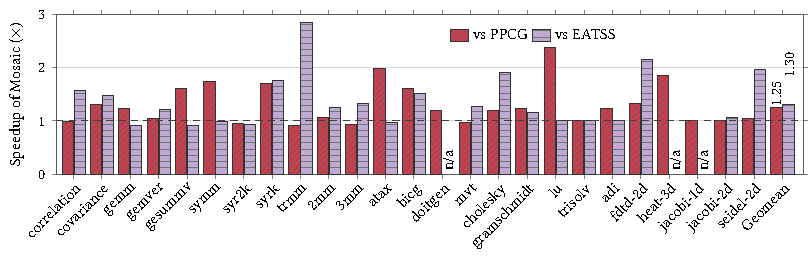
\includegraphics{figures/h800.pdf}
  \ifrevmarkup\captionsetup{labelfont+={color=revRone}}\fi
  \caption{\revRone{\name speedup over PPCG and EATSS on the H800.}}
  \label{fig:h800}
\end{figure}

\DIFaddend \subsection{Bounded PPCG Tile Sweep}
\label{subsec:bounded-ppcg-sweep}

To compare \name with an empirical tile search, we perform a deterministic bounded PPCG sweep containing 263--784 configurations per benchmark, sampled without regard to measured performance from three exhaustive classes: hardware-aligned powers of two, exact divisors of the problem size, and unaligned points. The sweep changes only tile sizes; PPCG continues to determine its block mapping and concrete shared-memory staging. Across the 25 benchmarks, we attempted 17,279 configurations and 15,960 compiled and executed successfully (92.37\%). Failures are dominated by CUDA resource-limit launch failures under PPCG's default block mapping, and failed points are excluded from the best-of-sweep result.

\begin{figure}[!b]
  \centering
  \setlength{\abovecaptionskip}{3pt}
  \DIFdelbeginFL %DIFDELCMD < \begin{tikzpicture}[trim axis left,trim axis right]
%DIFDELCMD <     \begin{axis}[
%DIFDELCMD <       ybar,
%DIFDELCMD <       width=0.86\linewidth,
%DIFDELCMD <       height=1.0cm,
%DIFDELCMD <       scale only axis,
%DIFDELCMD <       bar width=7pt,
%DIFDELCMD <       ymin=0.60,
%DIFDELCMD <       ymax=1.31,
%DIFDELCMD <       ytick={0.6,0.8,1.0,1.2},
%DIFDELCMD <       clip=false,
%DIFDELCMD <       ylabel={\(T_{\mathrm{sweep\text{-}best}} / T_{\mathrm{Mosaic}}\)},
%DIFDELCMD <       symbolic x coords={correlation,covariance,gemm,gemver,gesummv,symm,syr2k,syrk,trmm,2mm,3mm,atax,bicg,doitgen,mvt,cholesky,gramschmidt,lu,trisolv,adi,fdtd-2d,heat-3d,jacobi-1d,jacobi-2d,seidel-2d,Geomean},
%DIFDELCMD <       xtick=data,
%DIFDELCMD <       xticklabels={corr.,cov.,gemm,gmvr.,gsum.,symm,syr2k,syrk,trmm,2mm,3mm,atax,bicg,doit.,mvt,chol.,gram.,lu,tris.,adi,fdtd,heat,jac-1d,jac-2d,seidel,\textbf{GMean}},
%DIFDELCMD <       enlarge x limits=0.018,
%DIFDELCMD <       xticklabel style={rotate=30,anchor=east,font=\tiny},
%DIFDELCMD <       yticklabel style={font=\tiny},
%DIFDELCMD <       ylabel style={font=\tiny},
%DIFDELCMD <       ymajorgrids=true,
%DIFDELCMD <       grid style=dashed,
%DIFDELCMD <     ]
%DIFDELCMD <       \addplot[fill=color1,draw=black] table[x=benchmark,y=speedup] {bounded_sweep_data.dat};
%DIFDELCMD <       \draw[black,dashed,thick] (axis cs:correlation,1) -- (axis cs:Geomean,1);
%DIFDELCMD <       \node[font=\tiny,rotate=90,anchor=west,
%DIFDELCMD <             inner sep=0pt,outer sep=2pt]
%DIFDELCMD <         at (axis cs:Geomean,0.972809917) {\textbf{0.973\(\boldsymbol{\times}\)}};
%DIFDELCMD <     \end{axis}
%DIFDELCMD <   \end{tikzpicture}
%DIFDELCMD <   %%%
\DIFdelendFL \DIFaddbeginFL \begin{tikzpicture}[trim axis left,trim axis right]
    \begin{axis}[
      ybar,
      width=0.86\linewidth,
      height=1.0cm,
      scale only axis,
      bar width=7pt,
      ymin=0.60,
      ymax=1.31,
      ytick={0.6,0.8,1.0,1.2},
      clip=false,
      ylabel={\(T_{\mathrm{sweep\text{-}best}} / T_{\mathrm{Mosaic}}\)},
      symbolic x coords={correlation,covariance,gemm,gemver,gesummv,symm,syr2k,syrk,trmm,2mm,3mm,atax,bicg,doitgen,mvt,cholesky,gramschmidt,lu,trisolv,adi,fdtd-2d,heat-3d,jacobi-1d,jacobi-2d,seidel-2d,Geomean},
      xtick=data,
      xticklabels={corr.,cov.,gemm,gmvr.,gsum.,symm,syr2k,syrk,trmm,2mm,3mm,atax,bicg,doit.,mvt,chol.,gram.,lu,tris.,adi,fdtd,heat,jac-1d,jac-2d,seidel,\textbf{GMean}},
      enlarge x limits=0.018,
      xticklabel style={rotate=30,anchor=east,font=\tiny},
      yticklabel style={font=\tiny},
      ylabel style={font=\tiny},
      ymajorgrids=true,
      grid style=dashed,
    ]
      \addplot[fill=color1,draw=black] table[x=benchmark,y=speedup] {bounded_sweep_data.dat};
      \draw[black,dashed,thick] (axis cs:correlation,1) -- (axis cs:Geomean,1);
      \node[font=\tiny,anchor=south east,inner sep=1pt]
        at ([xshift=3pt]axis cs:Geomean,1.14) {\textbf{0.973\(\boldsymbol{\times}\)}};
    \end{axis}
  \end{tikzpicture}
  \DIFaddendFL \caption{\name{} speedup over bounded-sweep best on the RTX 4090; values above one favor \name{}.}
  \Description{Bar chart of bounded-sweep-best time divided by Mosaic time for 25 PolyBench benchmarks and their geometric mean. A dashed horizontal line marks parity at one, and the geometric mean is 0.973 times.}
  \label{fig:bounded-ppcg-sweep}
\end{figure}

The sweep deliberately extends beyond \name's analytical candidate set by including unaligned and non-divisor tile sizes. Sweep-best therefore serves as an empirical reference over the tested PPCG tile space rather than as the optimum of \name's own discrete domain. For each benchmark, we compute the fraction of successfully measured sweep configurations slower than PPCG's default and report the average of these fractions across all 25 benchmarks.

Across the 25 benchmarks, PPCG's default configuration outperforms 71.2\% of the successfully measured sweep configurations on average and exceeds the sweep median in 18 cases.

The sweep-best configurations achieve a $1.245\times$ geometric-mean speedup over this baseline, and beat it on all 25 benchmarks. \autoref{fig:bounded-ppcg-sweep} compares \name directly with sweep-best. The plotted ratio is \(T_{\mathrm{sweep\text{-}best}} / T_{\mathrm{Mosaic}}\): values above one favor \name and values below one favor sweep-best. The geometric-mean ratio is $0.973\times$, with \name faster on 12 of the 25 benchmarks and sweep-best faster on the remaining 13. Thus, \name reaches comparable aggregate performance without the hundreds of compile-and-run trials required by the bounded search for each benchmark.

\paragraph{Measured regret.}
The bounded sweep above varies tile sizes while retaining PPCG's block
mapping. We further evaluate how closely \name's analytical selection
approaches the best measured configuration when tile sizes and thread-block
dimensions are considered jointly. We define the measured regret as
\(T_{\name}/T_{\mathrm{best}}-1\), where \(T_{\mathrm{best}}\) is the fastest
configuration observed in the evaluated candidate space. For single-kernel
workloads, we exhaustively search the full feasible tile-and-block
configuration space to obtain the measured optimum; for multi-kernel
workloads, we control Cartesian-product growth by retaining the top-8 or
top-16 candidates per kernel according to analytical cost, limiting the
resulting joint search space to at most 512 configurations.

The measured regret is \(0.34\%\) for \texttt{trisolv}, \(20.59\%\) for
\texttt{syrk}, \(8.10\%\) for \texttt{gemm}, approximately \(0\%\) for
\texttt{atax}, and \(0.08\%\) for \texttt{fdtd-2d}, with a geometric mean
of \(5.53\%\). The larger regret on \texttt{syrk} indicates
a remaining mismatch in ranking block-shape and coalescing-sensitive
configurations.

\DIFaddbegin \revRthree{Extending the analysis to covariance, mvt, trmm, and jacobi-2d yields regrets of 2.52\%, 2.91\%, 7.74\%, and 13.34\%, for a nine-kernel geometric mean of 5.98\%. For syrk, the measured-best configuration lies in $\mathcal{V}(S)$ but needs more waves, so the model ranks it lower; Nsight Compute shows similar achieved occupancy for both but about 1/16 as many shared-memory read bank conflicts for the measured best. For jacobi-2d, the model counts each tile's halo (Eq.~\eqref{eq:stencil-halo}) but not the L2 reuse of halos shared by adjacent tiles. Bank conflicts depend on how the backend lays out staged tiles and maps threads onto them, and halo reuse on how concurrently resident blocks share L2; the current compiler-agnostic cost model represents neither.}

\DIFaddend \subsection{Performance on Deep Learning Operators}
\label{subsec:operators}

\DIFdelbegin %DIFDELCMD < \begin{wrapfigure}[11]{R}{0.49\textwidth}
%DIFDELCMD < %%%
\DIFdelend \DIFaddbegin \begin{wrapfigure}[13]{R}{0.49\textwidth}
\DIFaddend \centering
\DIFdelbegin %DIFDELCMD < \begin{tikzpicture}
%DIFDELCMD < \begin{groupplot}[
%DIFDELCMD <     group style={
%DIFDELCMD <         group size=1 by 2,
%DIFDELCMD <         vertical sep=3pt,
%DIFDELCMD <         xticklabels at=edge bottom,
%DIFDELCMD <     },
%DIFDELCMD <     ybar,
%DIFDELCMD <     /pgf/bar width=5pt,
%DIFDELCMD <     width=0.43\textwidth,
%DIFDELCMD <     symbolic x coords={CNN,LSTM,RNN,FNN,Embed},
%DIFDELCMD <     xtick=data,
%DIFDELCMD <     enlarge x limits=0.13,
%DIFDELCMD <     ymajorgrids=true,
%DIFDELCMD <     grid style=dashed,
%DIFDELCMD <     xticklabel style={font=\scriptsize, text depth=0pt},
%DIFDELCMD <     yticklabel style={font=\scriptsize},
%DIFDELCMD < ]
%DIFDELCMD <

%DIFDELCMD < \nextgroupplot[
%DIFDELCMD <     height=2.35cm,
%DIFDELCMD <     ymin=3, ymax=7.8,
%DIFDELCMD <     ytick={4.00,6.00}, yticklabels={4.00,6.00},
%DIFDELCMD <     legend style={
%DIFDELCMD <         at={(0.56,0.61)}, anchor=center,
%DIFDELCMD <         legend columns=2, font=\scriptsize,
%DIFDELCMD <         draw=none, fill=none,
%DIFDELCMD <         /tikz/every even column/.append style={column sep=0.15cm},
%DIFDELCMD <     },
%DIFDELCMD < ]
%DIFDELCMD < \addplot[fill=color1, draw=black, bar shift=-3.5pt] coordinates {
%DIFDELCMD <     (CNN,1)[] (LSTM,1)[] (RNN,1)[] (FNN,1)[] (Embed,1)[]
%DIFDELCMD < };
%DIFDELCMD < \addplot[
%DIFDELCMD <     fill=color4,
%DIFDELCMD <     draw=black,
%DIFDELCMD <     bar shift=3.5pt,
%DIFDELCMD < ] coordinates {
%DIFDELCMD <     (CNN,5.734)[]
%DIFDELCMD <     (LSTM,1.015)[]
%DIFDELCMD <     (RNN,1.035)[]
%DIFDELCMD <     (FNN,1.002)[]
%DIFDELCMD <     (Embed,3.853)[]
%DIFDELCMD < };
%DIFDELCMD < \legend{PPCG, \name}
%DIFDELCMD <

%DIFDELCMD < \nextgroupplot[
%DIFDELCMD <     height=3.25cm,
%DIFDELCMD <     ymin=0.980, ymax=1.145,
%DIFDELCMD <     ytick={1.00,1.04,1.08},
%DIFDELCMD <     yticklabels={1.00,1.04,1.08},
%DIFDELCMD < ]
%DIFDELCMD < \addplot[
%DIFDELCMD <     fill=color1,
%DIFDELCMD <     draw=black,
%DIFDELCMD <     bar shift=-3.5pt,
%DIFDELCMD <     nodes near coords,
%DIFDELCMD <     point meta=explicit symbolic,
%DIFDELCMD <     every node near coord/.append style={
%DIFDELCMD <         font=\tiny,
%DIFDELCMD <         rotate=90,
%DIFDELCMD <         anchor=west,
%DIFDELCMD <         inner sep=0pt,
%DIFDELCMD <         transform canvas={yshift=1.5pt},
%DIFDELCMD <     },
%DIFDELCMD < ] coordinates {
%DIFDELCMD <     (CNN,1)[549.69\,ms]
%DIFDELCMD <     (LSTM,1)[1010.2\,ms]
%DIFDELCMD <     (RNN,1)[1452.4\,ms]
%DIFDELCMD <     (FNN,1)[1.6980\,ms]
%DIFDELCMD <     (Embed,1)[544.26\,ms]
%DIFDELCMD < };
%DIFDELCMD < \addplot[
%DIFDELCMD <     fill=color4,
%DIFDELCMD <     draw=black,
%DIFDELCMD <     bar shift=3.5pt,
%DIFDELCMD <     nodes near coords,
%DIFDELCMD <     point meta=explicit symbolic,
%DIFDELCMD <     every node near coord/.append style={
%DIFDELCMD <         font=\tiny,
%DIFDELCMD <         rotate=90,
%DIFDELCMD <         anchor=west,
%DIFDELCMD <         inner sep=0pt,
%DIFDELCMD <         transform canvas={yshift=1.5pt},
%DIFDELCMD <     },
%DIFDELCMD < ] coordinates {
%DIFDELCMD <     (CNN,5.734)[]
%DIFDELCMD <     (LSTM,1.015)[$\mathbf{1.015}\mathbf{\times}$]
%DIFDELCMD <     (RNN,1.035)[$\mathbf{1.035}\mathbf{\times}$]
%DIFDELCMD <     (FNN,1.002)[$\mathbf{1.002}\mathbf{\times}$]
%DIFDELCMD <     (Embed,3.853)[]
%DIFDELCMD < };
%DIFDELCMD < % Keep the two values clipped by the broken axis in the lower panel.  Their
%DIFDELCMD < % identical y coordinate gives them the same vertical placement, while the
%DIFDELCMD < % explicit bar shift aligns each label with the center of its Mosaic bar.
%DIFDELCMD < \node[font=\tiny, rotate=90, anchor=west, inner sep=0pt]
%DIFDELCMD <     at ([xshift=3.5pt]axis cs:CNN,1.055)
%DIFDELCMD <     {$\mathbf{5.734}\mathbf{\times}$};
%DIFDELCMD < \node[font=\tiny, rotate=90, anchor=west, inner sep=0pt]
%DIFDELCMD <     at ([xshift=3.5pt]axis cs:Embed,1.055)
%DIFDELCMD <     {$\mathbf{3.853}\mathbf{\times}$};
%DIFDELCMD < \end{groupplot}
%DIFDELCMD <

%DIFDELCMD < \coordinate (bl) at ($(group c1r1.south west)!0.5!(group c1r2.north west)$);
%DIFDELCMD < \coordinate (br) at ($(group c1r1.south east)!0.5!(group c1r2.north east)$);
%DIFDELCMD < \foreach \p in {bl,br}{
%DIFDELCMD <     \draw[white,line width=2pt] ($(\p)+(0,-3pt)$)--($(\p)+(0,3pt)$);
%DIFDELCMD <     \draw[line width=.5pt] ($(\p)+(-3pt,-3pt)$)--($(\p)+(3pt,0pt)$);
%DIFDELCMD <     \draw[line width=.5pt] ($(\p)+(-3pt,0pt)$)--($(\p)+(3pt,3pt)$);
%DIFDELCMD < }
%DIFDELCMD <

%DIFDELCMD < \node[rotate=90, anchor=south, font=\scriptsize]
%DIFDELCMD <     at ([xshift=-20pt, yshift=-7pt]$(group c1r1.west)!0.5!(group c1r2.west)$)
%DIFDELCMD <     {Execution time speedup};
%DIFDELCMD < \end{tikzpicture}
%DIFDELCMD < %%%
\DIFdelend \DIFaddbegin 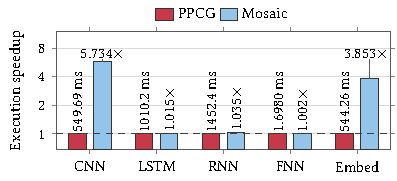
\includegraphics[width=\linewidth,height=92pt,keepaspectratio]{figures/operator_bars.pdf}
\DIFaddend \caption{Performance of deep learning operators.}
\Description{Bar chart comparing PPCG and \name speedups on CNN, LSTM, RNN, FNN, and embedding operators.}
\label{fig:network-operators}
\end{wrapfigure}

The remaining experiments on deep learning operators, end-to-end workloads, and ablation are conducted on the RTX 4090; \autoref{subsec:polybench} provides the cross-architecture evaluation on PolyBench. We next evaluate \name on five deep learning operators: CNN, LSTM, and RNN from the PolyNN suite~\cite{polynn}, and FNN and Embedding extracted from the AlexNet~\cite{alexnet} and BERT~\cite{bert}, respectively. \autoref{fig:network-operators} reports the speedup. \name delivers large gains on CNN (\(5.73\times\)) and Embedding (\(3.85\times\)) and remains within \(4\%\) of PPCG on LSTM, RNN, and FNN, yielding a geometric-mean speedup of \(1.88\times\).

These operators cover distinct regimes. CNN and FNN are contraction/GEMM-like and compute-intensive, where the \(\phi\) ratio of \autoref{sec:cost} most effectively trades locality against register pressure, but FNN is small and regular enough that the PPCG default already lands close to \name's configuration. LSTM is a memory-intensive recurrent operator whose performance is dominated more by data movement than arithmetic intensity, leaving less room for register-blocking trade-offs. Embedding is likewise data-movement dominated, but PPCG's default parameters leave substantial opportunity for \name's placement-aware and occupancy reasoning to improve the configuration under the fixed mapping.

For a direct comparison with optimized reference libraries, \autoref{tab:vendor-comparison} reports the audited CUDA-event medians for five GEMM shapes and the CNN case, with relative performance defined as reference-library time divided by Mosaic time. The GEMM geometric-mean ratios are \(67.65\%\) for FP64 and \(24.93\%\) for FP32. The reference measurements use cuBLAS for GEMM and cuDNN for CNN; the FP32 cuBLAS path uses FP32 input/output with TF32 Tensor-Core computation, whereas Mosaic uses scalar FP32 FMA.

\begin{table}[!t]
\centering
\caption{Mosaic and vendor execution time for GEMM and CNN. CNN shape
(\(\dagger\)): \(N=64\), \(C=64\), \(H=W=100\), \(K=32\), \(R=S=3\), and
\(P=Q=98\), with unit stride.}
\label{tab:vendor-comparison}
\scriptsize
\setlength{\tabcolsep}{2.5pt}
\renewcommand{\arraystretch}{1.04}
\begin{tabular*}{\textwidth}{@{\extracolsep{\fill}}llrrrrrr@{}}
\toprule
\multirow{2}{*}{Kernel} & \multirow{2}{*}{Shape} &
  \multicolumn{3}{c}{FP64} &
  \multicolumn{3}{c}{FP32 / TF32} \\
\cmidrule(lr){3-5}\cmidrule(lr){6-8}
& & Mosaic (ms) & Vendor (ms) & Perf. (\%)
  & Mosaic (ms) & Vendor (ms) & Perf. (\%) \\
\midrule
\multirow{6}{*}{GEMM}
& \(1024\times1024\times1024\) & 2.9062 & 1.9123 & 65.80 & 0.1421 & 0.0369 & 26.00 \\
& \(2048\times2048\times2048\) & 22.119 & 15.244 & 68.92 & 0.9138 & 0.2284 & 24.99 \\
& \(4096\times4096\times4096\) & 167.52 & 113.11 & 67.52 & 6.9988 & 1.7730 & 25.33 \\
& \(4096\times1024\times4096\) & 42.559 & 30.406 & 71.44 & 1.8401 & 0.4491 & 24.40 \\
& \(1024\times4096\times4096\) & 44.821 & 29.037 & 64.79 & 1.8609 & 0.4458 & 23.95 \\
& Geometric mean & -- & -- & 67.65 & -- & -- & 24.93 \\
\midrule
CNN\(^{\dagger}\) & -- & 7.1729 & 7.4175 & 103.4 & 7.9247 & 4.9041 & 61.88 \\
\bottomrule
\end{tabular*}
\end{table}

\DIFaddbegin \revO{On the RTX 4090, Tensor Cores accelerate TF32 but not FP64. In FP64, cuBLAS reaches 87\%--94\% of peak and the \name-selected PPCG kernels 57\%--64\%; the gap stems from library techniques such as multi-stage pipelining, vectorized accesses, and register prefetching, which lie outside tile and block selection. In FP32, the TF32 Tensor Core and FP32 CUDA-core peaks are both 82.6 TFLOPS, but each MMA instruction amortizes instruction and operand-fetch overhead over many multiply--adds; FP64 arithmetic hides this overhead in scalar kernels, whereas in FP32 it limits them to 18\%--24\% of peak. Most kernels in Table~\ref{tab:benchmark}, such as stencils, triangular solves, and matrix--vector reductions, cannot use Tensor Cores or have no vendor implementation, as is also the case for FP64 code on GPUs without FP64 Tensor Cores.}

\revO{\textit{Comparison with TileMind.} TileMind selects only tile sizes, from which PPCG derives the thread block, and its cost model omits discrete waves (\autoref{sec:related}). On the same PPCG backend in FP64, \name achieves geometric-mean speedups of 1.26$\times$ on GEMM and 2.44$\times$ on Conv2D over TileMind (Table~\ref{tab:tilemind}). The largest speedup, 10.21$\times$, occurs on a convolution for which the block derived from TileMind's tile holds a single warp, whereas \name selects 1,024 threads per block, so that many more threads share the input and weight tiles staged in shared memory.}

\begin{table}[tbp]
\centering
\ifrevmarkup\captionsetup{labelfont+={color=revO}}\fi
\caption{\revO{\name and TileMind execution time for GEMM and Conv2D. GEMM shapes are $M{\times}N{\times}K$; Conv2D shapes are input $N{\times}C{\times}H{\times}W$ $\rightarrow$ output $N{\times}K{\times}P{\times}Q$, with unit stride and no padding.}}\label{tab:tilemind}
\begin{revOblock}
\scriptsize
\setlength{\tabcolsep}{2.5pt}
\renewcommand{\arraystretch}{1.04}
\begin{tabular*}{\textwidth}{@{\extracolsep{\fill}}llrrr@{}}
\toprule
\DIFaddFL{Kernel }& \DIFaddFL{Shape }& \DIFaddFL{Mosaic (ms) }& \DIFaddFL{TileMind (ms) }& \DIFaddFL{Spd. }\\
\midrule
\multirow{6}{*}{GEMM} & \DIFaddFL{$768{\times}768{\times}128$ }& \DIFaddFL{0.176 }& \DIFaddFL{0.220 }& \DIFaddFL{1.25$\times$ }\\
 & \DIFaddFL{$384{\times}1536{\times}512$ }& \DIFaddFL{0.697 }& \DIFaddFL{0.869 }& \DIFaddFL{1.25$\times$ }\\
 & \DIFaddFL{$768{\times}768{\times}1536$ }& \DIFaddFL{2.082 }& \DIFaddFL{2.603 }& \DIFaddFL{1.25$\times$ }\\
 & \DIFaddFL{$1536{\times}1024{\times}768$ }& \DIFaddFL{2.546 }& \DIFaddFL{3.448 }& \DIFaddFL{1.35$\times$ }\\
 & \DIFaddFL{$1152{\times}1152{\times}1152$ }& \DIFaddFL{3.511 }& \DIFaddFL{4.176 }& \DIFaddFL{1.19$\times$ }\\
 & \DIFaddFL{Geometric mean }& \DIFaddFL{-- }& \DIFaddFL{-- }& \DIFaddFL{1.26$\times$ }\\
\midrule
\multirow{6}{*}{Conv2D} & \DIFaddFL{$4{\times}16{\times}18{\times}18\;\rightarrow\;4{\times}64{\times}16{\times}16$ }& \DIFaddFL{0.422 }& \DIFaddFL{0.514 }& \DIFaddFL{1.22$\times$ }\\
 & \DIFaddFL{$16{\times}32{\times}18{\times}18\;\rightarrow\;16{\times}32{\times}16{\times}16$ }& \DIFaddFL{1.706 }& \DIFaddFL{2.707 }& \DIFaddFL{1.59$\times$ }\\
 & \DIFaddFL{$24{\times}16{\times}18{\times}18\;\rightarrow\;24{\times}64{\times}16{\times}16$ }& \DIFaddFL{1.180 }& \DIFaddFL{12.049 }& \DIFaddFL{10.21$\times$ }\\
 & \DIFaddFL{$16{\times}32{\times}16{\times}16\;\rightarrow\;16{\times}64{\times}14{\times}14$ }& \DIFaddFL{2.078 }& \DIFaddFL{5.434 }& \DIFaddFL{2.61$\times$ }\\
 & \DIFaddFL{$16{\times}64{\times}16{\times}16\;\rightarrow\;16{\times}32{\times}14{\times}14$ }& \DIFaddFL{2.685 }& \DIFaddFL{4.503 }& \DIFaddFL{1.68$\times$ }\\
 & \DIFaddFL{Geometric mean }& \DIFaddFL{-- }& \DIFaddFL{-- }& \DIFaddFL{2.44$\times$ }\\
\bottomrule
\end{tabular*}
\end{revOblock}
\end{table}

\DIFaddend To compare \name against search-based autotuning, we integrate it into TVM~\cite{tvm} and compare with MetaSchedule~\cite{metaschedule} across trial budgets. \autoref{fig:network-operator-curves} plots execution time and selection cost for six operators. \name's overhead is a single compile-time analytical solve: for each modeled placement scenario in \(\Sigma\) it assembles one Stage-1 MILP and applies a relaxed-cost tie-break over the Stage-1 optimal discrete configurations (\autoref{sec:solver}), incurred once without generating or running any kernel. MetaSchedule's overhead is instead a runtime measurement loop: every trial compiles a kernel with NVCC and times it on the GPU, so the tuning cost grows linearly with the trial budget and is repaid for each new shape or target. \DIFaddbegin \revRthree{Fig.~\ref{fig:network-operator-curves} reports MetaSchedule's full tuning time because each of its trials samples tile sizes jointly with the other schedule decisions, so the parameter search cannot be timed separately; \name's solve time covers re-selecting tile/block sizes on the resulting schedule (\autoref{sec:eval}).} \DIFaddend Our comparison targets tile/block sizes; even when MetaSchedule is restricted to this choice under a fixed schedule\DIFaddbegin \revRthree{ with the same trial budgets}\DIFaddend , its overhead stays the same order of magnitude, since the dominant cost is compiling and running each candidate. One two-stage analytical selection pass replaces hundreds to thousands of compile-and-run trials, the source of the gap of two to four orders of magnitude in \autoref{fig:network-operator-curves}.

\begin{figure}[!htbp]
\centering
\definecolor{curveMosaic}{HTML}{CC0000}
\definecolor{curveTVM}{HTML}{FF6666}
\definecolor{curveSolverMosaic}{HTML}{0066CC}
\definecolor{curveSolverTVM}{HTML}{4D94E6}
\DIFdelbeginFL %DIFDELCMD < \resizebox{0.85\textwidth}{!}{%
%DIFDELCMD < \begin{tikzpicture}
%DIFDELCMD < \begin{scope}[xshift=0.125\columnwidth, yshift=4.30cm]
%DIFDELCMD < \begin{axis}[
%DIFDELCMD <     width=0.34\columnwidth, height=3.35cm,
%DIFDELCMD <     yticklabel style={color=curveMosaic, font=\scriptsize},
%DIFDELCMD <     ymode=log,
%DIFDELCMD <     ymin=1, ymax=100,
%DIFDELCMD <     ytick={1,10,100},
%DIFDELCMD <     xmode=log,
%DIFDELCMD <     xmin=0.8, xmax=1200,
%DIFDELCMD <     xtick={1,10,100,1000},
%DIFDELCMD <     xticklabels={1,$10^1$,$10^2$,$10^3$},
%DIFDELCMD <     xticklabel style={font=\scriptsize},
%DIFDELCMD <     grid=major,
%DIFDELCMD <     grid style={line width=0.3pt, draw=gray!25},
%DIFDELCMD <     axis y line*=left,
%DIFDELCMD <     axis x line*=bottom,
%DIFDELCMD <     title={CNN},
%DIFDELCMD <     title style={font=\footnotesize, yshift=-0.2cm},
%DIFDELCMD < ]
%DIFDELCMD < \addplot[color=curveMosaic, line width=0.55pt, solid, mark=*, mark size=1.2pt] coordinates {
%DIFDELCMD <     (1,4.2312) (10,4.2312) (100,4.2312) (200,4.2312) (500,4.2312) (1000,4.2312)
%DIFDELCMD < };
%DIFDELCMD < \addplot[color=curveTVM, line width=0.55pt, solid, mark=square*, mark size=1.2pt] coordinates {
%DIFDELCMD <     (1,51.732) (10,60.3056) (100,6.7591) (200,6.8391) (500,7.4544) (1000,5.8638)
%DIFDELCMD < };
%DIFDELCMD < \end{axis}
%DIFDELCMD < \begin{axis}[
%DIFDELCMD <     width=0.34\columnwidth, height=3.35cm,
%DIFDELCMD <     axis y line*=right,
%DIFDELCMD <     axis x line=none,
%DIFDELCMD <     yticklabel style={color=curveSolverMosaic, opacity=0},
%DIFDELCMD <     ymode=log,
%DIFDELCMD <     ymin=0.1, ymax=1000,
%DIFDELCMD <     ytick={0.1,10,1000},
%DIFDELCMD <     xmode=log,
%DIFDELCMD <     xmin=0.8, xmax=1200,
%DIFDELCMD < ]
%DIFDELCMD < \addplot[color=curveSolverMosaic, line width=0.55pt, dashed, mark=*, mark size=1.2pt] coordinates {
%DIFDELCMD <     (1,2.9676) (10,2.9676) (100,2.9676) (200,2.9676) (500,2.9676) (1000,2.9676)
%DIFDELCMD < };
%DIFDELCMD < \addplot[color=curveSolverTVM, line width=0.55pt, dashed, mark=square*, mark size=1.2pt] coordinates {
%DIFDELCMD <     (1,17.2) (10,42.3) (100,737.7) (200,939.3) (500,924.3) (1000,1078)
%DIFDELCMD < };
%DIFDELCMD < \end{axis}
%DIFDELCMD < \end{scope}
%DIFDELCMD <

%DIFDELCMD < \begin{scope}[xshift=0.440\columnwidth, yshift=4.30cm]
%DIFDELCMD < \begin{axis}[
%DIFDELCMD <     width=0.34\columnwidth, height=3.35cm,
%DIFDELCMD <     yticklabel style={color=curveMosaic, font=\scriptsize},
%DIFDELCMD <     ymode=log,
%DIFDELCMD <     ymin=0.1, ymax=100,
%DIFDELCMD <     ytick={0.1,1,10},
%DIFDELCMD <     xmode=log,
%DIFDELCMD <     xmin=0.8, xmax=1200,
%DIFDELCMD <     xtick={1,10,100,1000},
%DIFDELCMD <     xticklabels={1,$10^1$,$10^2$,$10^3$},
%DIFDELCMD <     xticklabel style={font=\scriptsize},
%DIFDELCMD <     grid=major,
%DIFDELCMD <     grid style={line width=0.3pt, draw=gray!25},
%DIFDELCMD <     axis y line*=left,
%DIFDELCMD <     axis x line*=bottom,
%DIFDELCMD <     title={LSTM},
%DIFDELCMD <     title style={font=\footnotesize, yshift=-0.2cm},
%DIFDELCMD < ]
%DIFDELCMD < \addplot[color=curveMosaic, line width=0.55pt, solid, mark=*, mark size=1.2pt] coordinates {
%DIFDELCMD <     (1,0.2332) (10,0.2332) (100,0.2332) (200,0.2332) (500,0.2332) (1000,0.2332)
%DIFDELCMD < };
%DIFDELCMD < \addplot[color=curveTVM, line width=0.55pt, solid, mark=square*, mark size=1.2pt] coordinates {
%DIFDELCMD <     (1,21.9229) (10,1.5843) (100,0.2814) (200,0.3319) (500,0.2185) (1000,0.2185)
%DIFDELCMD < };
%DIFDELCMD < \end{axis}
%DIFDELCMD < \begin{axis}[
%DIFDELCMD <     width=0.34\columnwidth, height=3.35cm,
%DIFDELCMD <     axis y line*=right,
%DIFDELCMD <     axis x line=none,
%DIFDELCMD <     yticklabel style={color=curveSolverMosaic, opacity=0},
%DIFDELCMD <     ymode=log,
%DIFDELCMD <     ymin=0.01, ymax=2000,
%DIFDELCMD <     ytick={0.01,10,1000},
%DIFDELCMD <     xmode=log,
%DIFDELCMD <     xmin=0.8, xmax=1200,
%DIFDELCMD < ]
%DIFDELCMD < \addplot[color=curveSolverMosaic, line width=0.55pt, dashed, mark=*, mark size=1.2pt] coordinates {
%DIFDELCMD <     (1,0.0741) (10,0.0741) (100,0.0741) (200,0.0741) (500,0.0741) (1000,0.0741)
%DIFDELCMD < };
%DIFDELCMD < \addplot[color=curveSolverTVM, line width=0.55pt, dashed, mark=square*, mark size=1.2pt] coordinates {
%DIFDELCMD <     (1,16) (10,22.47) (100,131.84) (200,267.54) (500,660.27) (1000,1326.86)
%DIFDELCMD < };
%DIFDELCMD < \end{axis}
%DIFDELCMD < \end{scope}
%DIFDELCMD <

%DIFDELCMD < \begin{scope}[xshift=0.755\columnwidth, yshift=4.30cm]
%DIFDELCMD < \begin{axis}[
%DIFDELCMD <     width=0.34\columnwidth, height=3.35cm,
%DIFDELCMD <     yticklabel style={color=curveMosaic, font=\scriptsize},
%DIFDELCMD <     ymode=log,
%DIFDELCMD <     ymin=10, ymax=3000,
%DIFDELCMD <     ytick={10,100,1000},
%DIFDELCMD <     xmode=log,
%DIFDELCMD <     xmin=0.8, xmax=1200,
%DIFDELCMD <     xtick={1,10,100,1000},
%DIFDELCMD <     xticklabels={1,$10^1$,$10^2$,$10^3$},
%DIFDELCMD <     xticklabel style={font=\scriptsize},
%DIFDELCMD <     grid=major,
%DIFDELCMD <     grid style={line width=0.3pt, draw=gray!25},
%DIFDELCMD <     axis y line*=left,
%DIFDELCMD <     axis x line*=bottom,
%DIFDELCMD <     title={RNN},
%DIFDELCMD <     title style={font=\footnotesize, yshift=-0.2cm},
%DIFDELCMD < ]
%DIFDELCMD < \addplot[color=curveMosaic, line width=0.55pt, solid, mark=*, mark size=1.2pt] coordinates {
%DIFDELCMD <     (1,20.4271) (10,20.4271) (100,20.4271) (200,20.4271) (500,20.4271) (1000,20.4271)
%DIFDELCMD < };
%DIFDELCMD < \addplot[color=curveTVM, line width=0.55pt, solid, mark=square*, mark size=1.2pt] coordinates {
%DIFDELCMD <     (1,2252.1594) (10,81.9091) (100,21.8536) (200,20.0876) (500,17.8522) (1000,17.7766)
%DIFDELCMD < };
%DIFDELCMD < \end{axis}
%DIFDELCMD < \begin{axis}[
%DIFDELCMD <     width=0.34\columnwidth, height=3.35cm,
%DIFDELCMD <     axis y line*=right,
%DIFDELCMD <     axis x line=none,
%DIFDELCMD <     yticklabel style={color=curveSolverMosaic, font=\scriptsize},
%DIFDELCMD <     ymode=log,
%DIFDELCMD <     ymin=0.1, ymax=2000,
%DIFDELCMD <     ytick={0.1,10,1000},
%DIFDELCMD <     xmode=log,
%DIFDELCMD <     xmin=0.8, xmax=1200,
%DIFDELCMD < ]
%DIFDELCMD < \addplot[color=curveSolverMosaic, line width=0.55pt, dashed, mark=*, mark size=1.2pt] coordinates {
%DIFDELCMD <     (1,0.716) (10,0.716) (100,0.716) (200,0.716) (500,0.716) (1000,0.716)
%DIFDELCMD < };
%DIFDELCMD < \addplot[color=curveSolverTVM, line width=0.55pt, dashed, mark=square*, mark size=1.2pt] coordinates {
%DIFDELCMD <     (1,23.44) (10,219.66) (100,823.3) (200,895.68) (500,1007.83) (1000,1012.12)
%DIFDELCMD < };
%DIFDELCMD < \end{axis}
%DIFDELCMD < \end{scope}
%DIFDELCMD <

%DIFDELCMD < \begin{scope}[xshift=0.125\columnwidth, yshift=1.65cm]
%DIFDELCMD < \begin{axis}[
%DIFDELCMD <     width=0.34\columnwidth, height=3.35cm,
%DIFDELCMD <     yticklabel style={color=curveMosaic, font=\scriptsize},
%DIFDELCMD <     ymode=log,
%DIFDELCMD <     ymin=0.05, ymax=2,
%DIFDELCMD <     ytick={0.05,0.2,1},
%DIFDELCMD <     xmode=log,
%DIFDELCMD <     xmin=0.8, xmax=1200,
%DIFDELCMD <     xtick={1,10,100,1000},
%DIFDELCMD <     xticklabels={1,$10^1$,$10^2$,$10^3$},
%DIFDELCMD <     xticklabel style={font=\scriptsize},
%DIFDELCMD <     grid=major,
%DIFDELCMD <     grid style={line width=0.3pt, draw=gray!25},
%DIFDELCMD <     axis y line*=left,
%DIFDELCMD <     axis x line*=bottom,
%DIFDELCMD <     title={FNN},
%DIFDELCMD <     title style={font=\footnotesize, yshift=-0.2cm},
%DIFDELCMD < ]
%DIFDELCMD < \addplot[color=curveMosaic, line width=0.55pt, solid, mark=*, mark size=1.2pt] coordinates {
%DIFDELCMD <     (1,0.0738) (10,0.0738) (100,0.0738) (200,0.0738) (500,0.0738) (1000,0.0738)
%DIFDELCMD < };
%DIFDELCMD < \addplot[color=curveTVM, line width=0.55pt, solid, mark=square*, mark size=1.2pt] coordinates {
%DIFDELCMD <     (1,0.9439) (10,1.2417) (100,0.1618) (200,0.0944) (500,0.081) (1000,0.0741)
%DIFDELCMD < };
%DIFDELCMD < \end{axis}
%DIFDELCMD < \begin{axis}[
%DIFDELCMD <     width=0.34\columnwidth, height=3.35cm,
%DIFDELCMD <     axis y line*=right,
%DIFDELCMD <     axis x line=none,
%DIFDELCMD <     yticklabel style={color=curveSolverMosaic, opacity=0},
%DIFDELCMD <     ymode=log,
%DIFDELCMD <     ymin=0.01, ymax=1000,
%DIFDELCMD <     ytick={0.01,1,100},
%DIFDELCMD <     xmode=log,
%DIFDELCMD <     xmin=0.8, xmax=1200,
%DIFDELCMD < ]
%DIFDELCMD < \addplot[color=curveSolverMosaic, line width=0.55pt, dashed, mark=*, mark size=1.2pt] coordinates {
%DIFDELCMD <     (1,0.1194) (10,0.1194) (100,0.1194) (200,0.1194) (500,0.1194) (1000,0.1194)
%DIFDELCMD < };
%DIFDELCMD < \addplot[color=curveSolverTVM, line width=0.55pt, dashed, mark=square*, mark size=1.2pt] coordinates {
%DIFDELCMD <     (1,9.8) (10,15.2) (100,78.2) (200,122.8) (500,282.5) (1000,561.9)
%DIFDELCMD < };
%DIFDELCMD < \end{axis}
%DIFDELCMD < \end{scope}
%DIFDELCMD <

%DIFDELCMD < \begin{scope}[xshift=0.440\columnwidth, yshift=1.65cm]
%DIFDELCMD < \begin{axis}[
%DIFDELCMD <     width=0.34\columnwidth, height=3.35cm,
%DIFDELCMD <     yticklabel style={color=curveMosaic, font=\scriptsize},
%DIFDELCMD <     ymode=log,
%DIFDELCMD <     ymin=10, ymax=500,
%DIFDELCMD <     ytick={10,50,200},
%DIFDELCMD <     xmode=log,
%DIFDELCMD <     xmin=0.8, xmax=1200,
%DIFDELCMD <     xtick={1,10,100,1000},
%DIFDELCMD <     xticklabels={1,$10^1$,$10^2$,$10^3$},
%DIFDELCMD <     xticklabel style={font=\scriptsize},
%DIFDELCMD <     grid=major,
%DIFDELCMD <     grid style={line width=0.3pt, draw=gray!25},
%DIFDELCMD <     axis y line*=left,
%DIFDELCMD <     axis x line*=bottom,
%DIFDELCMD <     title={Embedding},
%DIFDELCMD <     title style={font=\footnotesize, yshift=-0.2cm},
%DIFDELCMD < ]
%DIFDELCMD < \addplot[color=curveMosaic, line width=0.55pt, solid, mark=*, mark size=1.2pt] coordinates {
%DIFDELCMD <     (1,12.9526) (10,12.9526) (100,12.9526) (200,12.9526) (500,12.9526) (1000,12.9526)
%DIFDELCMD < };
%DIFDELCMD < \addplot[color=curveTVM, line width=0.55pt, solid, mark=square*, mark size=1.2pt] coordinates {
%DIFDELCMD <     (1,362.8838) (10,85.9239) (100,38.2759) (200,32.3857) (500,29.9019) (1000,25.491)
%DIFDELCMD < };
%DIFDELCMD < \end{axis}
%DIFDELCMD < \begin{axis}[
%DIFDELCMD <     width=0.34\columnwidth, height=3.35cm,
%DIFDELCMD <     axis y line*=right,
%DIFDELCMD <     axis x line=none,
%DIFDELCMD <     yticklabel style={color=curveSolverMosaic, opacity=0},
%DIFDELCMD <     ymode=log,
%DIFDELCMD <     ymin=0.01, ymax=3000,
%DIFDELCMD <     ytick={0.01,10,1000},
%DIFDELCMD <     xmode=log,
%DIFDELCMD <     xmin=0.8, xmax=1200,
%DIFDELCMD < ]
%DIFDELCMD < \addplot[color=curveSolverMosaic, line width=0.55pt, dashed, mark=*, mark size=1.2pt] coordinates {
%DIFDELCMD <     (1,0.3567) (10,0.3567) (100,0.3567) (200,0.3567) (500,0.3567) (1000,0.3567)
%DIFDELCMD < };
%DIFDELCMD < \addplot[color=curveSolverTVM, line width=0.55pt, dashed, mark=square*, mark size=1.2pt] coordinates {
%DIFDELCMD <     (1,16.71) (10,108.89) (100,610.7) (200,1041.74) (500,2432.51) (1000,2432.51)
%DIFDELCMD < };
%DIFDELCMD < \end{axis}
%DIFDELCMD < \end{scope}
%DIFDELCMD <

%DIFDELCMD < \begin{scope}[xshift=0.755\columnwidth, yshift=1.65cm]
%DIFDELCMD < \begin{axis}[
%DIFDELCMD <     width=0.34\columnwidth, height=3.35cm,
%DIFDELCMD <     yticklabel style={color=curveMosaic, font=\scriptsize},
%DIFDELCMD <     ymode=log,
%DIFDELCMD <     ymin=1, ymax=50,
%DIFDELCMD <     ytick={1,5,20},
%DIFDELCMD <     xmode=log,
%DIFDELCMD <     xmin=0.8, xmax=1200,
%DIFDELCMD <     xtick={1,10,100,1000},
%DIFDELCMD <     xticklabels={1,$10^1$,$10^2$,$10^3$},
%DIFDELCMD <     xticklabel style={font=\scriptsize},
%DIFDELCMD <     grid=major,
%DIFDELCMD <     grid style={line width=0.3pt, draw=gray!25},
%DIFDELCMD <     axis y line*=left,
%DIFDELCMD <     axis x line*=bottom,
%DIFDELCMD <     title={Matmul},
%DIFDELCMD <     title style={font=\footnotesize, yshift=-0.2cm},
%DIFDELCMD < ]
%DIFDELCMD < \addplot[color=curveMosaic, line width=0.55pt, solid, mark=*, mark size=1.2pt] coordinates {
%DIFDELCMD <     (1,4.4347) (10,4.4347) (100,4.4347) (200,4.4347) (500,4.4347) (1000,4.4347)
%DIFDELCMD < };
%DIFDELCMD < \addplot[color=curveTVM, line width=0.55pt, solid, mark=square*, mark size=1.2pt] coordinates {
%DIFDELCMD <     (1,26.5995) (10,20.8549) (100,7.149) (200,4.2035) (500,4.5826) (1000,4.1599)
%DIFDELCMD < };
%DIFDELCMD < \end{axis}
%DIFDELCMD < \begin{axis}[
%DIFDELCMD <     width=0.34\columnwidth, height=3.35cm,
%DIFDELCMD <     axis y line*=right,
%DIFDELCMD <     axis x line=none,
%DIFDELCMD <     yticklabel style={color=curveSolverMosaic, font=\scriptsize},
%DIFDELCMD <     ymode=log,
%DIFDELCMD <     ymin=0.01, ymax=2000,
%DIFDELCMD <     ytick={0.01,10,1000},
%DIFDELCMD <     xmode=log,
%DIFDELCMD <     xmin=0.8, xmax=1200,
%DIFDELCMD < ]
%DIFDELCMD < \addplot[color=curveSolverMosaic, line width=0.55pt, dashed, mark=*, mark size=1.2pt] coordinates {
%DIFDELCMD <     (1,0.21) (10,0.21) (100,0.21) (200,0.21) (500,0.21) (1000,0.21)
%DIFDELCMD < };
%DIFDELCMD < \addplot[color=curveSolverTVM, line width=0.55pt, dashed, mark=square*, mark size=1.2pt] coordinates {
%DIFDELCMD <     (1,11.06) (10,88.17) (100,360.63) (200,601.6) (500,866.03) (1000,1671.5)
%DIFDELCMD < };
%DIFDELCMD < \end{axis}
%DIFDELCMD < \end{scope}
%DIFDELCMD <

%DIFDELCMD < \node[rotate=90, color=curveMosaic, font=\scriptsize] at (0.020\columnwidth, 3.25cm) {Execution time (ms)};
%DIFDELCMD < \node[rotate=90, color=curveSolverMosaic, font=\scriptsize] at (1.100\columnwidth, 3.25cm) {Search/solver (s)};
%DIFDELCMD < \node[font=\scriptsize] at (0.560\columnwidth, 0.72cm) {Number of Trials};
%DIFDELCMD < \node at (0.560\columnwidth, -0.02cm) {
%DIFDELCMD <     \begin{tikzpicture}
%DIFDELCMD <         % Mosaic exec.
%DIFDELCMD <         \draw[color=curveMosaic, line width=0.7pt, solid] (0,0) -- (0.28,0);
%DIFDELCMD <         \filldraw[fill=curveMosaic, draw=white, line width=0.3pt]
%DIFDELCMD <             (0.16,0) circle (0.045);
%DIFDELCMD <         \node[right, font=\footnotesize] at (0.34,0) {Mosaic exec.};
%DIFDELCMD <

%DIFDELCMD <         % TVM exec.
%DIFDELCMD <         \draw[color=curveTVM, line width=0.7pt, solid] (2.05,0) -- (2.33,0);
%DIFDELCMD <         \filldraw[fill=curveTVM, draw=white, line width=0.3pt]
%DIFDELCMD <             (2.16,-0.05) rectangle (2.26,0.05);
%DIFDELCMD <         \node[right, font=\footnotesize] at (2.37,0) {TVM exec.};
%DIFDELCMD <

%DIFDELCMD <         % Mosaic solver
%DIFDELCMD <         \draw[color=curveSolverMosaic, line width=0.7pt, dashed] (3.85,0) -- (4.13,0);
%DIFDELCMD <         \filldraw[fill=curveSolverMosaic, draw=white, line width=0.3pt]
%DIFDELCMD <             (4.01,0) circle (0.045);
%DIFDELCMD <         \node[right, font=\footnotesize] at (4.19,0) {Mosaic solver};
%DIFDELCMD <

%DIFDELCMD <         % TVM search
%DIFDELCMD <         \draw[color=curveSolverTVM, line width=0.7pt, dashed] (6.10,0) -- (6.38,0);
%DIFDELCMD <         \filldraw[fill=curveSolverTVM, draw=white, line width=0.3pt]
%DIFDELCMD <             (6.21,-0.05) rectangle (6.31,0.05);
%DIFDELCMD <         \node[right, font=\footnotesize] at (6.44,0) {TVM search};
%DIFDELCMD <     }
%DIFDELCMD < \end{tikzpicture};
%DIFDELCMD <

%DIFDELCMD < % Reset to symmetric bounds so labels cannot bias the six-panel composition.
%DIFDELCMD < \pgfresetboundingbox
%DIFDELCMD < \path[use as bounding box] (-0.031\columnwidth,-0.25cm) rectangle (1.151\columnwidth,6.35cm);
%DIFDELCMD <

%DIFDELCMD < \end{tikzpicture}
%DIFDELCMD < }
%DIFDELCMD < %%%
\DIFdelendFL \DIFaddbeginFL \resizebox{0.85\textwidth}{!}{%
\begin{tikzpicture}
\begin{scope}[xshift=0.125\columnwidth, yshift=4.30cm]
\begin{axis}[
    width=0.321\columnwidth, height=3.35cm,
    yticklabel style={color=curveMosaic, font=\scriptsize},
    ymode=log,
    ymin=1, ymax=100,
    ytick={1,10,100},
    yticklabels={$10^{0}$,$10^{1}$,$10^{2}$},
    xmode=log,
    xmin=0.8, xmax=1200,
    xtick={1,10,100,1000},
    xticklabels={1,$10^1$,$10^2$,$10^3$},
    xticklabel style={font=\scriptsize},
    grid=major,
    grid style={line width=0.3pt, draw=gray!25},
    axis y line*=left,
    axis x line*=bottom,
    title={CNN},
    title style={font=\footnotesize, yshift=-0.2cm},
]
\addplot[color=curveMosaic, line width=0.55pt, solid, mark=*, mark size=1.2pt] coordinates {
    (1,4.2312) (10,4.2312) (100,4.2312) (200,4.2312) (500,4.2312) (1000,4.2312)
};
\addplot[color=curveTVM, line width=0.55pt, solid, mark=square*, mark size=1.2pt] coordinates {
    (1,51.732) (10,60.3056) (100,6.7591) (200,6.8391) (500,7.4544) (1000,5.8638)
};
\end{axis}
\begin{axis}[
    width=0.321\columnwidth, height=3.35cm,
    axis y line*=right,
    axis x line=none,
    yticklabel style={color=curveSolverMosaic, font=\scriptsize},
    ymode=log,
    ymin=0.1, ymax=1200,
    ytick={0.1,10,1000},
    yticklabels={$10^{-1}$,$10^{1}$,$10^{3}$},
    xmode=log,
    xmin=0.8, xmax=1200,
]
\addplot[color=curveSolverMosaic, line width=0.55pt, dashed, mark=*, mark size=1.2pt] coordinates {
    (1,2.9676) (10,2.9676) (100,2.9676) (200,2.9676) (500,2.9676) (1000,2.9676)
};
\addplot[color=curveSolverTVM, line width=0.55pt, dashed, mark=square*, mark size=1.2pt] coordinates {
    (1,17.2) (10,42.3) (100,737.7) (200,939.3) (500,924.3) (1000,1078)
};
\end{axis}
\end{scope}

\begin{scope}[xshift=0.440\columnwidth, yshift=4.30cm]
\begin{axis}[
    width=0.321\columnwidth, height=3.35cm,
    yticklabel style={color=curveMosaic, font=\scriptsize},
    ymode=log,
    ymin=0.1, ymax=100,
    ytick={0.1,1,10},
    yticklabels={$10^{-1}$,$10^{0}$,$10^{1}$},
    xmode=log,
    xmin=0.8, xmax=1200,
    xtick={1,10,100,1000},
    xticklabels={1,$10^1$,$10^2$,$10^3$},
    xticklabel style={font=\scriptsize},
    grid=major,
    grid style={line width=0.3pt, draw=gray!25},
    axis y line*=left,
    axis x line*=bottom,
    title={LSTM},
    title style={font=\footnotesize, yshift=-0.2cm},
]
\addplot[color=curveMosaic, line width=0.55pt, solid, mark=*, mark size=1.2pt] coordinates {
    (1,0.2332) (10,0.2332) (100,0.2332) (200,0.2332) (500,0.2332) (1000,0.2332)
};
\addplot[color=curveTVM, line width=0.55pt, solid, mark=square*, mark size=1.2pt] coordinates {
    (1,21.9229) (10,1.5843) (100,0.2814) (200,0.3319) (500,0.2185) (1000,0.2185)
};
\end{axis}
\begin{axis}[
    width=0.321\columnwidth, height=3.35cm,
    axis y line*=right,
    axis x line=none,
    yticklabel style={color=curveSolverMosaic, font=\scriptsize},
    ymode=log,
    ymin=0.01, ymax=2000,
    ytick={0.01,10,1000},
    yticklabels={$10^{-2}$,$10^{1}$,$10^{3}$},
    xmode=log,
    xmin=0.8, xmax=1200,
]
\addplot[color=curveSolverMosaic, line width=0.55pt, dashed, mark=*, mark size=1.2pt] coordinates {
    (1,0.0741) (10,0.0741) (100,0.0741) (200,0.0741) (500,0.0741) (1000,0.0741)
};
\addplot[color=curveSolverTVM, line width=0.55pt, dashed, mark=square*, mark size=1.2pt] coordinates {
    (1,16) (10,22.47) (100,131.84) (200,267.54) (500,660.27) (1000,1326.86)
};
\end{axis}
\end{scope}

\begin{scope}[xshift=0.755\columnwidth, yshift=4.30cm]
\begin{axis}[
    width=0.321\columnwidth, height=3.35cm,
    yticklabel style={color=curveMosaic, font=\scriptsize},
    ymode=log,
    ymin=10, ymax=3000,
    ytick={10,100,1000},
    yticklabels={$10^{1}$,$10^{2}$,$10^{3}$},
    xmode=log,
    xmin=0.8, xmax=1200,
    xtick={1,10,100,1000},
    xticklabels={1,$10^1$,$10^2$,$10^3$},
    xticklabel style={font=\scriptsize},
    grid=major,
    grid style={line width=0.3pt, draw=gray!25},
    axis y line*=left,
    axis x line*=bottom,
    title={RNN},
    title style={font=\footnotesize, yshift=-0.2cm},
]
\addplot[color=curveMosaic, line width=0.55pt, solid, mark=*, mark size=1.2pt] coordinates {
    (1,20.4271) (10,20.4271) (100,20.4271) (200,20.4271) (500,20.4271) (1000,20.4271)
};
\addplot[color=curveTVM, line width=0.55pt, solid, mark=square*, mark size=1.2pt] coordinates {
    (1,2252.1594) (10,81.9091) (100,21.8536) (200,20.0876) (500,17.8522) (1000,17.7766)
};
\end{axis}
\begin{axis}[
    width=0.321\columnwidth, height=3.35cm,
    axis y line*=right,
    axis x line=none,
    yticklabel style={color=curveSolverMosaic, font=\scriptsize},
    ymode=log,
    ymin=0.1, ymax=2000,
    ytick={0.1,10,1000},
    yticklabels={$10^{-1}$,$10^{1}$,$10^{3}$},
    xmode=log,
    xmin=0.8, xmax=1200,
]
\addplot[color=curveSolverMosaic, line width=0.55pt, dashed, mark=*, mark size=1.2pt] coordinates {
    (1,0.716) (10,0.716) (100,0.716) (200,0.716) (500,0.716) (1000,0.716)
};
\addplot[color=curveSolverTVM, line width=0.55pt, dashed, mark=square*, mark size=1.2pt] coordinates {
    (1,23.44) (10,219.66) (100,823.3) (200,895.68) (500,1007.83) (1000,1012.12)
};
\end{axis}
\end{scope}

\begin{scope}[xshift=0.125\columnwidth, yshift=1.65cm]
\begin{axis}[
    width=0.321\columnwidth, height=3.35cm,
    yticklabel style={color=curveMosaic, font=\scriptsize},
    ymode=log,
    ymin=0.05, ymax=2,
    ytick={0.1,1},
    yticklabels={$10^{-1}$,$10^{0}$},
    xmode=log,
    xmin=0.8, xmax=1200,
    xtick={1,10,100,1000},
    xticklabels={1,$10^1$,$10^2$,$10^3$},
    xticklabel style={font=\scriptsize},
    grid=major,
    grid style={line width=0.3pt, draw=gray!25},
    axis y line*=left,
    axis x line*=bottom,
    title={FNN},
    title style={font=\footnotesize, yshift=-0.2cm},
]
\addplot[color=curveMosaic, line width=0.55pt, solid, mark=*, mark size=1.2pt] coordinates {
    (1,0.0738) (10,0.0738) (100,0.0738) (200,0.0738) (500,0.0738) (1000,0.0738)
};
\addplot[color=curveTVM, line width=0.55pt, solid, mark=square*, mark size=1.2pt] coordinates {
    (1,0.9439) (10,1.2417) (100,0.1618) (200,0.0944) (500,0.081) (1000,0.0741)
};
\end{axis}
\begin{axis}[
    width=0.321\columnwidth, height=3.35cm,
    axis y line*=right,
    axis x line=none,
    yticklabel style={color=curveSolverMosaic, font=\scriptsize},
    ymode=log,
    ymin=0.01, ymax=1000,
    ytick={0.01,1,100},
    yticklabels={$10^{-2}$,$10^{0}$,$10^{2}$},
    xmode=log,
    xmin=0.8, xmax=1200,
]
\addplot[color=curveSolverMosaic, line width=0.55pt, dashed, mark=*, mark size=1.2pt] coordinates {
    (1,0.1194) (10,0.1194) (100,0.1194) (200,0.1194) (500,0.1194) (1000,0.1194)
};
\addplot[color=curveSolverTVM, line width=0.55pt, dashed, mark=square*, mark size=1.2pt] coordinates {
    (1,9.8) (10,15.2) (100,78.2) (200,122.8) (500,282.5) (1000,561.9)
};
\end{axis}
\end{scope}

\begin{scope}[xshift=0.440\columnwidth, yshift=1.65cm]
\begin{axis}[
    width=0.321\columnwidth, height=3.35cm,
    yticklabel style={color=curveMosaic, font=\scriptsize},
    ymode=log,
    ymin=10, ymax=500,
    ytick={10,100},
    yticklabels={$10^{1}$,$10^{2}$},
    xmode=log,
    xmin=0.8, xmax=1200,
    xtick={1,10,100,1000},
    xticklabels={1,$10^1$,$10^2$,$10^3$},
    xticklabel style={font=\scriptsize},
    grid=major,
    grid style={line width=0.3pt, draw=gray!25},
    axis y line*=left,
    axis x line*=bottom,
    title={Embedding},
    title style={font=\footnotesize, yshift=-0.2cm},
]
\addplot[color=curveMosaic, line width=0.55pt, solid, mark=*, mark size=1.2pt] coordinates {
    (1,12.9526) (10,12.9526) (100,12.9526) (200,12.9526) (500,12.9526) (1000,12.9526)
};
\addplot[color=curveTVM, line width=0.55pt, solid, mark=square*, mark size=1.2pt] coordinates {
    (1,362.8838) (10,85.9239) (100,38.2759) (200,32.3857) (500,29.9019) (1000,25.491)
};
\end{axis}
\begin{axis}[
    width=0.321\columnwidth, height=3.35cm,
    axis y line*=right,
    axis x line=none,
    yticklabel style={color=curveSolverMosaic, font=\scriptsize},
    ymode=log,
    ymin=0.01, ymax=3000,
    ytick={0.01,10,1000},
    yticklabels={$10^{-2}$,$10^{1}$,$10^{3}$},
    xmode=log,
    xmin=0.8, xmax=1200,
]
\addplot[color=curveSolverMosaic, line width=0.55pt, dashed, mark=*, mark size=1.2pt] coordinates {
    (1,0.3567) (10,0.3567) (100,0.3567) (200,0.3567) (500,0.3567) (1000,0.3567)
};
\addplot[color=curveSolverTVM, line width=0.55pt, dashed, mark=square*, mark size=1.2pt] coordinates {
    (1,16.71) (10,108.89) (100,610.7) (200,1041.74) (500,2432.51) (1000,2432.51)
};
\end{axis}
\end{scope}

\begin{scope}[xshift=0.755\columnwidth, yshift=1.65cm]
\begin{axis}[
    width=0.321\columnwidth, height=3.35cm,
    yticklabel style={color=curveMosaic, font=\scriptsize},
    ymode=log,
    ymin=1, ymax=50,
    ytick={1,10},
    yticklabels={$10^{0}$,$10^{1}$},
    xmode=log,
    xmin=0.8, xmax=1200,
    xtick={1,10,100,1000},
    xticklabels={1,$10^1$,$10^2$,$10^3$},
    xticklabel style={font=\scriptsize},
    grid=major,
    grid style={line width=0.3pt, draw=gray!25},
    axis y line*=left,
    axis x line*=bottom,
    title={Matmul},
    title style={font=\footnotesize, yshift=-0.2cm},
]
\addplot[color=curveMosaic, line width=0.55pt, solid, mark=*, mark size=1.2pt] coordinates {
    (1,4.4347) (10,4.4347) (100,4.4347) (200,4.4347) (500,4.4347) (1000,4.4347)
};
\addplot[color=curveTVM, line width=0.55pt, solid, mark=square*, mark size=1.2pt] coordinates {
    (1,26.5995) (10,20.8549) (100,7.149) (200,4.2035) (500,4.5826) (1000,4.1599)
};
\end{axis}
\begin{axis}[
    width=0.321\columnwidth, height=3.35cm,
    axis y line*=right,
    axis x line=none,
    yticklabel style={color=curveSolverMosaic, font=\scriptsize},
    ymode=log,
    ymin=0.01, ymax=2000,
    ytick={0.01,10,1000},
    yticklabels={$10^{-2}$,$10^{1}$,$10^{3}$},
    xmode=log,
    xmin=0.8, xmax=1200,
]
\addplot[color=curveSolverMosaic, line width=0.55pt, dashed, mark=*, mark size=1.2pt] coordinates {
    (1,0.21) (10,0.21) (100,0.21) (200,0.21) (500,0.21) (1000,0.21)
};
\addplot[color=curveSolverTVM, line width=0.55pt, dashed, mark=square*, mark size=1.2pt] coordinates {
    (1,11.06) (10,88.17) (100,360.63) (200,601.6) (500,866.03) (1000,1671.5)
};
\end{axis}
\end{scope}

\node[rotate=90, color=curveMosaic, font=\scriptsize] at (0.020\columnwidth, 3.25cm) {Execution time (ms)};
\node[rotate=90, color=curveSolverMosaic, font=\scriptsize] at (1.100\columnwidth, 3.25cm) {Search/solver (s)};
\node[font=\scriptsize] at (0.560\columnwidth, 0.72cm) {Number of Trials};
\node at (0.560\columnwidth, -0.02cm) {
    \begin{tikzpicture}
        % Mosaic exec.
        \draw[color=curveMosaic, line width=0.7pt, solid] (0,0) -- (0.28,0);
        \filldraw[fill=curveMosaic, draw=white, line width=0.3pt]
            (0.16,0) circle (0.045);
        \node[right, font=\footnotesize] at (0.34,0) {Mosaic exec.};

        % TVM exec.
        \draw[color=curveTVM, line width=0.7pt, solid] (2.05,0) -- (2.33,0);
        \filldraw[fill=curveTVM, draw=white, line width=0.3pt]
            (2.16,-0.05) rectangle (2.26,0.05);
        \node[right, font=\footnotesize] at (2.37,0) {TVM exec.};

        % Mosaic solver
        \draw[color=curveSolverMosaic, line width=0.7pt, dashed] (3.85,0) -- (4.13,0);
        \filldraw[fill=curveSolverMosaic, draw=white, line width=0.3pt]
            (4.01,0) circle (0.045);
        \node[right, font=\footnotesize] at (4.19,0) {Mosaic solver};

        % TVM search
        \draw[color=curveSolverTVM, line width=0.7pt, dashed] (6.10,0) -- (6.38,0);
        \filldraw[fill=curveSolverTVM, draw=white, line width=0.3pt]
            (6.21,-0.05) rectangle (6.31,0.05);
        \node[right, font=\footnotesize] at (6.44,0) {TVM search};
    }
\end{tikzpicture};

% Reset to symmetric bounds so labels cannot bias the six-panel composition.
\pgfresetboundingbox
\path[use as bounding box] (-0.031\columnwidth,-0.25cm) rectangle (1.151\columnwidth,6.35cm);

\end{tikzpicture}
}
\DIFaddendFL \caption{Execution time and search/solver overhead for six operators, comparing with TVM MetaSchedule. Solid lines show execution time; dashed lines show selection cost.}
\Description{Six curve plots for CNN, LSTM, RNN, FNN, embedding, and matmul comparing \name and tvm SSSRRSRS execution time and search or solver overhead.}
\label{fig:network-operator-curves}
\end{figure}

\autoref{fig:network-operator-curves} includes a sixth operator, Matmul, scheduled from TVM metadata; \texttt{tvm.relay.nn.matmul} is a first-class operator with native MetaSchedule support, extending the evaluation to a standalone dense contraction. The PPCG side covers the same case through the GEMM kernel of \autoref{subsec:polybench}, so Matmul is not repeated in \autoref{fig:network-operators}.

% Keep Fig. 6 before the next subsection without forcing a new page.
\FloatBarrier
\subsection{Performance on End-to-End Workloads}
\label{subsec:e2e}

% Match the half-width presentation used by Fig. 8 and keep this figure inside
% the end-to-end subsection.  The explicit line count prevents the wrap from
% carrying into the following subsection.
\DIFdelbegin %DIFDELCMD < \begin{wrapfigure}[10]{r}{0.49\textwidth}
%DIFDELCMD < %%%
\DIFdelend \DIFaddbegin \begin{wrapfigure}[12]{r}{0.49\textwidth}
\DIFaddend \centering
\DIFdelbegin %DIFDELCMD < \begin{tikzpicture}
%DIFDELCMD < \definecolor{figSevenPurple}{RGB}{181,145,204}
%DIFDELCMD < \begin{groupplot}[
%DIFDELCMD <     group style={
%DIFDELCMD <         group size=1 by 2,
%DIFDELCMD <         vertical sep=3pt,
%DIFDELCMD <         xticklabels at=edge bottom,
%DIFDELCMD <     },
%DIFDELCMD <     ybar,
%DIFDELCMD <     /pgf/bar width=4pt,
%DIFDELCMD <     width=\linewidth,
%DIFDELCMD <     xmin=-0.25,
%DIFDELCMD <     xmax=1.69,
%DIFDELCMD <     xtick={0,0.72,1.44},
%DIFDELCMD <     xticklabels={AlexNet,Seq2Seq,BertTiny},
%DIFDELCMD <     ymajorgrids=true,
%DIFDELCMD <     grid style=dashed,
%DIFDELCMD <     xticklabel style={font=\tiny},
%DIFDELCMD <     yticklabel style={font=\tiny},
%DIFDELCMD <     nodes near coords,
%DIFDELCMD <     every node near coord/.append style={
%DIFDELCMD <         font=\tiny,
%DIFDELCMD <         rotate=90,
%DIFDELCMD <         anchor=west
%DIFDELCMD <     },
%DIFDELCMD <     point meta=explicit symbolic,
%DIFDELCMD < ]
%DIFDELCMD < \nextgroupplot[
%DIFDELCMD <     height=2.42cm,
%DIFDELCMD <     ymin=1.4,
%DIFDELCMD <     ymax=13.5,
%DIFDELCMD <     % Affinely map the displayed [1.4,10] range onto the former [1.4,8]
%DIFDELCMD <     % range.  Thus the 10x tick occupies the former 8x position and the
%DIFDELCMD <     % space above it is reserved for the legend instead of covering bars.
%DIFDELCMD <     ytick={1.860465,4.162791,8.0},
%DIFDELCMD <     yticklabels={2,5,10},
%DIFDELCMD <     legend style={
%DIFDELCMD <         at={(axis cs:0.72,11.2)},
%DIFDELCMD <         anchor=center,
%DIFDELCMD <         legend columns=4,
%DIFDELCMD <         font=\tiny,
%DIFDELCMD <         draw=none,
%DIFDELCMD <         fill=none,
%DIFDELCMD <         /tikz/every even column/.append style={
%DIFDELCMD <             column sep=0.04cm
%DIFDELCMD <         },
%DIFDELCMD <     },
%DIFDELCMD < ]
%DIFDELCMD < \addplot[fill=color1,draw=black,bar shift=-9pt] coordinates {
%DIFDELCMD <     (0,1.093023)[]
%DIFDELCMD <     (0.72,1.093023)[]
%DIFDELCMD <     (1.44,1.093023)[]
%DIFDELCMD < };
%DIFDELCMD < \addplot[
%DIFDELCMD <     fill=figSevenPurple,
%DIFDELCMD <     draw=black,
%DIFDELCMD <     bar shift=-3pt
%DIFDELCMD < ] coordinates {
%DIFDELCMD <     (0,1.599535)[]
%DIFDELCMD <     (0.72,7.406767)[]
%DIFDELCMD <     (1.44,4.086047)[]
%DIFDELCMD < };
%DIFDELCMD < \addplot[fill=color2,draw=black,bar shift=3pt] coordinates {
%DIFDELCMD <     (0,1.093023)[]
%DIFDELCMD <     (0.72,1.093023)[]
%DIFDELCMD <     (1.44,1.093023)[]
%DIFDELCMD < };
%DIFDELCMD < \addplot[fill=color4,draw=black,bar shift=9pt] coordinates {
%DIFDELCMD <     (0,1.215047)[]
%DIFDELCMD <     (0.72,1.132930)[]
%DIFDELCMD <     (1.44,1.190488)[]
%DIFDELCMD < };
%DIFDELCMD <

%DIFDELCMD < \legend{PPCG, \name/PPCG, TVM, \name/TVM}
%DIFDELCMD < \nextgroupplot[
%DIFDELCMD <     height=2.5cm,
%DIFDELCMD <     ymin=0.9,
%DIFDELCMD <     % Headroom above the 1.20 tick so the rotated baseline-time and speedup
%DIFDELCMD <     % labels clear the panel border instead of colliding with the axis break.
%DIFDELCMD <     ymax=1.40,
%DIFDELCMD <     ytick={1.00,1.10,1.20},
%DIFDELCMD <     yticklabels={1.00,1.10,1.20},
%DIFDELCMD < ]
%DIFDELCMD <

%DIFDELCMD < \addplot[fill=color1,draw=black,bar shift=-9pt] coordinates {
%DIFDELCMD <     (0,1)[850.869ms]
%DIFDELCMD <     (0.72,1)[102720ms]
%DIFDELCMD <     (1.44,1)[226.710ms]
%DIFDELCMD < };
%DIFDELCMD < \addplot[fill=figSevenPurple,draw=black,bar shift=-3pt] coordinates {
%DIFDELCMD <     (0,1.660)[]
%DIFDELCMD <     (0.72,9.227)[]
%DIFDELCMD <     (1.44,4.900)[]
%DIFDELCMD < };
%DIFDELCMD < \addplot[fill=color2,draw=black,bar shift=3pt] coordinates {
%DIFDELCMD <     (0,1)[26.2720ms]
%DIFDELCMD <     (0.72,1)[614.433ms]
%DIFDELCMD <     (1.44,1)[5.40400ms]
%DIFDELCMD < };
%DIFDELCMD < \addplot[fill=color4,draw=black,bar shift=9pt] coordinates {
%DIFDELCMD <     (0,1.159)[\textbf{1.159$\times$}]
%DIFDELCMD <     (0.72,1.052)[\textbf{1.052$\times$}]
%DIFDELCMD <     (1.44,1.127)[\textbf{1.127$\times$}]
%DIFDELCMD < };
%DIFDELCMD < % Put all Mosaic/PPCG values inside the visible lower-axis portion of the
%DIFDELCMD < % second bar, with the same explicit -3pt shift used by that bar series.
%DIFDELCMD < \node[font=\tiny\bfseries\boldmath,rotate=90,anchor=east,inner sep=1pt]
%DIFDELCMD <     at ([xshift=-3pt]axis cs:0,1.36) {$1.660\times$};
%DIFDELCMD < \node[font=\tiny\bfseries\boldmath,rotate=90,anchor=east,inner sep=1pt]
%DIFDELCMD <     at ([xshift=-3pt]axis cs:0.72,1.36) {$9.227\times$};
%DIFDELCMD < \node[font=\tiny\bfseries\boldmath,rotate=90,anchor=east,inner sep=1pt]
%DIFDELCMD <     at ([xshift=-3pt]axis cs:1.44,1.36) {$4.900\times$};
%DIFDELCMD < \end{groupplot}
%DIFDELCMD < \coordinate (bl) at
%DIFDELCMD <     ($(group c1r1.south west)!0.5!(group c1r2.north west)$);
%DIFDELCMD < \coordinate (br) at
%DIFDELCMD <     ($(group c1r1.south east)!0.5!(group c1r2.north east)$);
%DIFDELCMD < \foreach \p in {bl,br}{
%DIFDELCMD <     \draw[white,line width=2pt]
%DIFDELCMD <         ($(\p)+(0,-3pt)$)--($(\p)+(0,3pt)$);
%DIFDELCMD <     \draw[line width=.5pt]
%DIFDELCMD <         ($(\p)+(-3pt,-3pt)$)--($(\p)+(3pt,0pt)$);
%DIFDELCMD <     \draw[line width=.5pt]
%DIFDELCMD <         ($(\p)+(-3pt,0pt)$)--($(\p)+(3pt,3pt)$);
%DIFDELCMD < }
%DIFDELCMD < \node[
%DIFDELCMD <     rotate=90,
%DIFDELCMD <     anchor=south,
%DIFDELCMD <     font=\scriptsize
%DIFDELCMD < ]
%DIFDELCMD < at (
%DIFDELCMD <     [xshift=-15pt,yshift=-0pt]
%DIFDELCMD <     $(group c1r1.west)!0.5!(group c1r2.west)$
%DIFDELCMD < ){Execution time speedup};
%DIFDELCMD < \end{tikzpicture}
%DIFDELCMD < %%%
\DIFdelend \DIFaddbegin 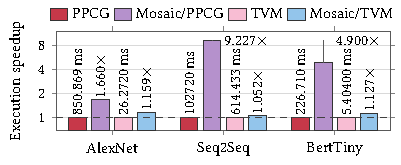
\includegraphics[width=\linewidth,height=81pt,keepaspectratio]{figures/network_bars.pdf}
\DIFaddend \caption{Performance of end-to-end workloads.}
\Description{
Four bars per network: PPCG baseline, \name{} over PPCG,
TVM baseline, and \name{} over TVM.
}
\label{fig:e2e-fourbar}
\end{wrapfigure}

We compose the operators into three end-to-end workloads spanning the major network families: AlexNet~\cite{alexnet} (CNN), Seq2Seq~\cite{lstm} (RNN), and BertTiny~\cite{bert} (Transformer). \DIFaddbegin \revO{In each comparison, both methods use the same network sizes, operator partitioning, execution order, and timing harness, without graph-level optimizations such as operator fusion, so only the kernels' execution parameters differ; \name selects them at compile time, and the network invokes the compiled kernels at run time.} \DIFaddend \autoref{fig:e2e-fourbar} reports the per-network speedup of \name over both PPCG and TVM, with baseline execution times shown left of the corresponding bars. Over PPCG, \name achieves $1.66\times$, $9.23\times$, and $4.90\times$ on AlexNet, Seq2Seq, and BertTiny (geometric mean $4.22\times$); over TVM MetaSchedule\DIFaddbegin \revRthree{'s tuned parameters on the same schedules}\DIFaddend , it achieves $1.16\times$, $1.05\times$, and $1.13\times$ (geometric mean $1.11\times$). In this fixed-schedule comparison, \name achieves slightly lower end-to-end latency than MetaSchedule without measurement-driven search, while improving substantially over PPCG's heuristic. The end-to-end gains over PPCG exceed the per-operator gains of \autoref{subsec:operators} because consistently good execution-space choices across consecutive layers compound into a larger overall improvement.

% Keep Fig. 7 inside the end-to-end subsection.
\FloatBarrier
\subsection{Ablation Study}
\label{subsec:ablation}

We ablate \name's three components cumulatively; FP-Wave keeps only the quantized wave objective (\autoref{sec:cost}) under a single fixed modeled placement scenario.

\begin{wrapfigure}[10]{R}{0.49\textwidth}
\centering
\DIFdelbegin %DIFDELCMD < \begin{tikzpicture}
%DIFDELCMD < \begin{axis}[
%DIFDELCMD <     ybar,
%DIFDELCMD <     /pgf/bar width=4pt,
%DIFDELCMD <     width=\linewidth,
%DIFDELCMD <     height=3.5cm,
%DIFDELCMD <     xmin=-0.36,
%DIFDELCMD <     xmax=3.24,
%DIFDELCMD <     xtick={0,0.72,1.44,2.16,2.88},
%DIFDELCMD <     xticklabels={covariance,syrk,3mm,gemm,cnn},
%DIFDELCMD <     ymin=0.8,
%DIFDELCMD <     ymax=4.0,
%DIFDELCMD <     ytick={1.0,1.5,2.0,2.5,3.0,3.5},
%DIFDELCMD <     yticklabels={1.0,1.5,2.0,2.5,3.0,3.5},
%DIFDELCMD <     ymajorgrids=true,
%DIFDELCMD <     grid style=dashed,
%DIFDELCMD <     xticklabel style={font=\scriptsize},
%DIFDELCMD <     yticklabel style={font=\scriptsize},
%DIFDELCMD <     ylabel={Execution time speedup},
%DIFDELCMD <     ylabel style={font=\scriptsize},
%DIFDELCMD <     nodes near coords,
%DIFDELCMD <     every node near coord/.append style={
%DIFDELCMD <         font=\tiny,
%DIFDELCMD <         rotate=90,
%DIFDELCMD <         anchor=west,
%DIFDELCMD <         inner sep=0pt
%DIFDELCMD <     },
%DIFDELCMD <     point meta=explicit symbolic,
%DIFDELCMD <     legend style={
%DIFDELCMD <         at={(0.5,0.98)}, anchor=north,
%DIFDELCMD <         legend columns=3, font=\scriptsize,
%DIFDELCMD <         draw=none, fill=none,
%DIFDELCMD <         /tikz/every even column/.append style={column sep=0.12cm}
%DIFDELCMD <     },
%DIFDELCMD < ]
%DIFDELCMD < \addplot[fill=color1, draw=black, bar shift=-6pt] coordinates {
%DIFDELCMD <     (0,1)[31.512ms]
%DIFDELCMD <     (0.72,1)[28.324ms]
%DIFDELCMD <     (1.44,1)[50.674ms]
%DIFDELCMD <     (2.16,1)[36.994ms]
%DIFDELCMD <     (2.88,1)[265.793ms]
%DIFDELCMD < };
%DIFDELCMD < \addplot[fill=color3, draw=black, bar shift=0pt] coordinates {
%DIFDELCMD <     (0,1.152)[\textbf{1.152$\times$}]
%DIFDELCMD <     (0.72,1.319)[\textbf{1.319$\times$}]
%DIFDELCMD <     (1.44,1.004)[\textbf{1.004$\times$}]
%DIFDELCMD <     (2.16,1.125)[\textbf{1.125$\times$}]
%DIFDELCMD <     (2.88,2.337)[]
%DIFDELCMD < };
%DIFDELCMD < \addplot[fill=color4, draw=black, bar shift=6pt] coordinates {
%DIFDELCMD <     (0,1.827)[]
%DIFDELCMD <     (0.72,1.439)[\textbf{1.439$\times$}]
%DIFDELCMD <     (1.44,1.556)[\textbf{1.556$\times$}]
%DIFDELCMD <     (2.16,1.630)[\textbf{1.630$\times$}]
%DIFDELCMD <     (2.88,2.773)[]
%DIFDELCMD < };
%DIFDELCMD < \legend{FP-Wave, RF-Wave, Mosaic}
%DIFDELCMD < \node[font=\tiny, rotate=90, anchor=center, inner sep=0pt] at ([xshift=6pt]axis cs:0,1.45) {\textbf{1.827$\times$}};
%DIFDELCMD < \node[font=\tiny, rotate=90, anchor=center, inner sep=0pt] at (axis cs:2.88,1.93) {\textbf{2.337$\times$}};
%DIFDELCMD < \node[font=\tiny, rotate=90, anchor=center, inner sep=0pt] at ([xshift=6pt]axis cs:2.88,2.28) {\textbf{2.773$\times$}};
%DIFDELCMD < \end{axis}
%DIFDELCMD < \end{tikzpicture}
%DIFDELCMD < %%%
\DIFdelend \DIFaddbegin 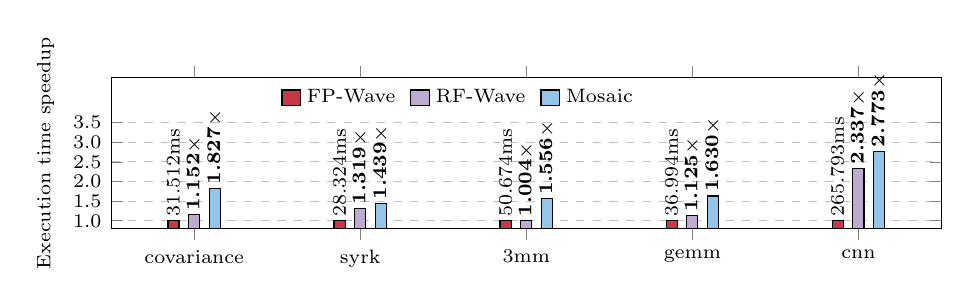
\begin{tikzpicture}
\begin{axis}[
    ybar, area legend,
    /pgf/bar width=4pt,
    width=\linewidth,
    height=3.5cm,
    xmin=-0.36,
    xmax=3.24,
    xtick={0,0.72,1.44,2.16,2.88},
    xticklabels={covariance,syrk,3mm,gemm,cnn},
    ymin=0.8,
    ymax=4.65,
    ytick={1.0,1.5,2.0,2.5,3.0,3.5},
    yticklabels={1.0,1.5,2.0,2.5,3.0,3.5},
    ymajorgrids=true,
    grid style=dashed,
    xticklabel style={font=\scriptsize},
    yticklabel style={font=\scriptsize},
    ylabel={Execution time speedup},
    ylabel style={font=\scriptsize},
    nodes near coords,
    every node near coord/.append style={
        font=\fontsize{7.5}{8.2}\selectfont,
        rotate=90,
        anchor=west,
        inner sep=1.3pt
    },
    point meta=explicit symbolic,
    legend style={
        at={(0.42,1.0)}, anchor=north,
        legend image post style={xscale=.40},
        legend columns=3, font=\scriptsize,
        draw=none, fill=none,
        /tikz/every even column/.append style={column sep=0.12cm}
    },
]
\addplot[fill=color1, draw=black, bar shift=-7.5pt] coordinates {
    (0,1)[31.512ms]
    (0.72,1)[28.324ms]
    (1.44,1)[50.674ms]
    (2.16,1)[36.994ms]
    (2.88,1)[265.793ms]
};
\addplot[fill=color3, draw=black, bar shift=0pt] coordinates {
    (0,1.152)[\textbf{1.152$\times$}]
    (0.72,1.319)[\textbf{1.319$\times$}]
    (1.44,1.004)[\textbf{1.004$\times$}]
    (2.16,1.125)[\textbf{1.125$\times$}]
    (2.88,2.337)[\textbf{2.337$\times$}]
};
\addplot[fill=color4, draw=black, bar shift=7.5pt] coordinates {
    (0,1.827)[\textbf{1.827$\times$}]
    (0.72,1.439)[\textbf{1.439$\times$}]
    (1.44,1.556)[\textbf{1.556$\times$}]
    (2.16,1.630)[\textbf{1.630$\times$}]
    (2.88,2.773)[\textbf{2.773$\times$}]
};
\legend{FP-Wave, RF-Wave, Mosaic}
\end{axis}
\end{tikzpicture}
\DIFaddend \caption{Ablation of \name's individual components.}
\Description{Grouped bar chart showing execution-time speedups of RF-Wave and Mosaic over the FP-Wave baseline on covariance, syrk, 3mm, gemm, and CNN.}
\label{fig:ablation}
\end{wrapfigure}

It disables both the register-feasibility filter and placement-scenario enumeration. RF-Wave adds the conservative register filter C4 while holding the modeled placement scenario fixed, isolating the filter's effect; full \name further enables placement-scenario enumeration over \(\Sigma\) (\autoref{sec:abstraction}), isolating the effect of placement-scenario reasoning. With FP-Wave as the baseline, RF-Wave improves performance by a geometric mean of $1.32\times$ and full \name by $1.79\times$, the largest gain on CNN, where filtering and placement-aware analytical reasoning together cut the selected configuration from $265.793$~ms to $95.851$~ms.

\subsection{Solver Overhead and Scalability}
\label{subsec:overhead}

Finally, we examine the cost of \name's analytical selection, reported in the solver-time columns of \autoref{tab:benchmark}. \DIFaddbegin \revO{For the PolyBench kernels in Table~\ref{tab:benchmark},} \DIFaddend \name completes its two-stage solving in well under one second for most kernels and at most a few seconds in the most demanding case (\texttt{syr2k} at $3.32$~s on the RTX 4090). The formulation introduces decision variables over the bounded candidate pairs of \autoref{sec:abstraction} and applies the resource constraints of \autoref{sec:constraints} within each per-scenario solve. Its model size is therefore determined by the discrete candidate counts and the small placement-scenario set, rather than by the number of dynamic loop iterations. Relative to EATSS, \name reduces selection overhead by arithmetic-mean factors of $12.6\times$, $13.6\times$, and $13.9\times$ on RTX 4090, A100, and V100; unlike the latency ratios, this comparison is unaffected by the objective mismatch, since both selectors are analytical. This one-time compile-time cost requires no runtime tuning loop and remains modest across the evaluated kernels.

\DIFaddbegin \revO{For a network, operators with identical structure and sizes share one solution, so \name's solving cost is the sum over its distinct operators and is incurred once at compile time: 26.6 s for AlexNet, 0.59 s for Seq2Seq, and 2.73 s for BertTiny. A new input shape requires re-solving because the candidates, grid size, and wave count change, but only the dimension sizes are updated; the schedule metadata and target profile are reused.}

\DIFaddend % !TEX root =  mosaic.tex
\section{Related Work}
\label{sec:related}

Existing approaches on optimizing loop nests and tensor programs can be broadly divided into \emph{schedule optimization} and \emph{execution space optimization}. While modern frameworks have extensively studied schedule optimization through polyhedral scheduling~\DIFdelbegin \DIFdel{\mbox{%DIFAUXCMD
\cite{ppcg,polly,tc,polygeist,akg}}\hspace{0pt}%DIFAUXCMD
}\DIFdelend \DIFaddbegin {\hypersetup{citecolor=black}[\citenum{polly}, \citenum{polygeist}, \citenum{tc}, \citenum{ppcg}, \revO{\citenum{zhao2020micro}}, \citenum{akg}]}\DIFaddend , including specialized tiling transformations for stencil computations~\cite{splitover,hybridtile,diamond}, and schedule-template search~\cite{halide,tvm}, execution space optimization remains dominated by heuristics and empirical tuning\DIFaddbegin \revO{~\cite{zhao2024tocs}}\DIFaddend . \name is a member of the second class only: it consumes a transformation schedule already fixed by one of these upstream systems and never searches or revises it, so it is complementary to, rather than competing with, schedule optimization.

\par\noindent\hspace*{\parindent}\textit{Analytical optimization.} Analytical tile size selection has a long history on CPUs~\cite{mckinley-tss,lam-tss,pingali-tss,tss-revisited}, later formulated using polynomial~\cite{pluto-tss} or geometric programming~\cite{rajopadhye-gp,rajopadhye-igp} within frameworks such as Pluto~\cite{pluto}, PPCG~\cite{ppcg}, and PolyMage~\cite{polymage}, or decoupled from compiler internals through an MILP formulation by TileMind~\cite{tilemind}. These methods target CPU cache residency and focus on tile sizes alone.

\DIFaddbegin \revO{TileMind~\cite{tilemind} likewise decouples its analytical model from compiler internals and formulates tile-size selection as an MILP, but solves a different problem: in its GPU validation it selects only tile sizes, from which PPCG derives thread-block dimensions, and its cost model omits discrete waves. \name jointly selects tile sizes and thread-block dimensions and models their coupling through residency, the register working set, shared-memory placement, and wave quantization; \autoref{subsec:operators} compares the two empirically.}

\DIFaddend GPU execution space optimization is more challenging because tile sizes interact with thread-block configurations, shared-memory allocation, occupancy, and register pressure. A recent work~\cite{ppcg-tss} incorporates tile-size selection into PPCG's scheduling formulation, while EATSS~\cite{eatss} analytically models GPU tiling using a joint latency--energy objective rather than latency alone. Among published analytical GPU tile-size selectors with available implementations, EATSS provides the closest baseline in scope to \name\DIFdelbegin \DIFdel{; TileMind targets CPU cache residency rather than GPU execution-space selection}\DIFdelend . \name applies a compiler-agnostic analytical core to compiler-provided schedule metadata through compiler-specific adapters.

\par\noindent\hspace*{\parindent}\textit{Kernel-specific models.} Several analytical models target specific kernels such as GEMM and convolution~\cite{anatomy,li-gemm,blis,saday-conv,conv-cache}, achieving high accuracy but generalizing poorly. \name instead targets a broader class of affine kernels, including contractions, reductions, and stencil computations.

\par\noindent\hspace*{\parindent}\textit{Search-based optimization.} Modern systems increasingly rely on empirical search: early kernel-specific autotuners such as PHiPAC and ATLAS explore parameters for dense linear algebra~\cite{phipac,atlas}, OpenTuner composes general search techniques~\cite{opentuner}, and more recent systems such as Ansor~\cite{ansor}, MetaSchedule~\cite{metaschedule}, and related tuners for Halide~\cite{automatichalide} and Triton~\cite{triton} generate and evaluate many candidate configurations. Learning-based and dynamic-programming approaches further approximate this space with predictive models or recursive search~\DIFdelbegin \DIFdel{\mbox{%DIFAUXCMD
\cite{hctuner,yuki-tss,Jangda2020dp,shirako-tss}}\hspace{0pt}%DIFAUXCMD
}\DIFdelend \DIFaddbegin {\hypersetup{citecolor=black}[\citenum{hctuner}, \citenum{Jangda2020dp}, \citenum{shirako-tss}, \citenum{yuki-tss}, \revO{\citenum{zhai2024tlm}}]}\DIFaddend ; all can be viewed as alternative ways of exploring the same execution-space optimization problem.

Rather than searching over configurations, \name directly models GPU resource interactions and solves for execution parameters analytically; \autoref{sec:eval} compares it against the PPCG heuristic, the energy-aware EATSS analytical selector, and the search-based MetaSchedule.

% !TEX root =  mosaic.tex
\section{Conclusion}
\label{sec:conclusion}

We presented \name, a unified analytical framework for GPU execution-space optimization. \name selects tile sizes and thread-block dimensions while reasoning over abstract shared-memory placement scenarios and accounting for occupancy and register pressure. Its two-stage analytical selection preserves the quantized primary optimum and uses a relaxed-cost tie-break only among tied legal discrete configurations, including across modeled placement scenarios, so \name selects these parameters without generating and evaluating large numbers of GPU kernels. Experimental results include a cross-generation PolyBench evaluation on three NVIDIA GPUs, together with deep learning operators and end-to-end workloads on the RTX 4090. Across these experiments, \name achieves geometric-mean speedups over PPCG, lower aggregate latency relative to EATSS, and slightly higher end-to-end performance than \DIFaddbegin \revRthree{with the parameters tuned by }\DIFaddend TVM MetaSchedule at substantially lower optimization overhead, suggesting that architecture-aware execution-space optimization can be addressed analytically rather than through measurement-driven search.

\name operates after transformation scheduling: it preserves the upstream schedule and mapping structure, selects tile and thread-block parameters, and leaves concrete shared-memory staging to the backend. The current model uses the loop and access metadata described in \autoref{sec:metadata} and targets conventional CUDA-core SIMT execution, as evaluated through the PPCG and non-tensorized TVM paths in this work\DIFaddbegin \revO{, which generate neither Tensor Core MMA instructions nor warp-specialized pipelines and leave PTX/SASS instruction selection and scheduling to NVCC/PTXAS}\DIFaddend . Extending the formulation to irregular accesses and tensorized or asynchronous execution requires corresponding resource models and metadata.


\bibliographystyle{ACM-Reference-Format}
\bibliography{references}

%DIF <  \appendix
%DIF <  \input{sec.apdx}
%DIF >  Appendix omitted.

\end{document}
\endinput
